\documentclass[11pt]{article}
\usepackage[utf8]{inputenc}
\usepackage[dvipsnames]{xcolor}
\usepackage{tikz}
\usepackage{fancyvrb}
\usepackage{enumitem}
\usepackage{hhline}
\usepackage{colortbl}
\usepackage{placeins}
\usepackage{hyperref}
\usepackage{booktabs, multirow} % for borders and merged ranges
\usepackage{soul}% for underlines
\usepackage{changepage,threeparttable} % for wide tables
\topmargin=-0.45in
\evensidemargin=0in
\oddsidemargin=0in
\textwidth=6.5in
\textheight=9.0in
\headsep=0.25in
\begin{document}

\input{titlepage} 

\newpage

% \section*{Part 1 [25 points]}

Using the instructions provided in the project description, run memcached alone (i.e., no interference), and with each iBench source of interference (cpu, l1d, l1i, l2, llc, membw). For Part 1, you must use the following \texttt{mcperf} command, which varies the target QPS from 30000 to 110000 in increments of 5000 (and has a warm-up time of 2 seconds with the addition of \texttt{-w 2}):

\begin{verbatim}
$ ./mcperf -s MEMCACHED_IP --loadonly
$ ./mcperf -s MEMCACHED_IP -a INTERNAL_AGENT_IP  \
           --noload -T 16 -C 4 -D 4 -Q 1000 -c 4 -w 2 -t 5 \ 
           --scan 30000:110000:5000
\end{verbatim}

\noindent Repeat the run for each of the 7 configurations (without interference, and the 6 interference types) \textbf{at least three times} (three should be sufficient in this case), and collect the performance measurements (i.e., the \texttt{client-measure} VM output). Reminder: after you have collected all the measurements, make sure you \underline{delete your cluster}. Otherwise, you will easily use up the cloud credits. See the project description for instructions how.

%%%%%%%%%%%%%%%%%%%%%%%%%%%%%%%%%%%%%%%%%%%
%%% QUESTION 1A

\begin{enumerate}[label=(\alph*)]
    \setcounter{enumi}{0}

    \item \textbf{[10 points]} Plot a single line graph with the following stipulations:
    \begin{itemize}
        \item Queries per second (QPS) on the x-axis (the x-axis should range from 0 to 110K).\\
        (note: the actual achieved QPS, not the target QPS)
        \item 95th percentile latency on the y-axis (the y-axis should range from 0 to 8 ms).
        \item Label your axes.
        \item 7 lines, one for each configuration. Add a legend.
        \item State how many runs you averaged across and include error bars at each point in both dimensions.
        \item The readability of your plot will be part of your grade.
    \end{itemize}
    
    % \textbf{The shape of the curves depends on many factors and may differ across groups. However, that does not imply that your solutions are wrong.}
    \textbf{Solution:} In order to plot the graph we averaged three different runs: as we only have three measurements the error bars represent the minimum and maximum measurements taken, while the point represents the average. We could represent the error bars as the standard deviation but with our approach we do not lose information in the measurements as they are represented directly in the graph. For the sake of readability, we averaged several measurements with achieved QPS very similar one to another in the \texttt{l1i} and \texttt{cpu} benchmarks as they struggle to reach more than 50K we would have an agglomerate of points there. In this way, we do not have too many points concentrated in the same area of the graph thus improving readability. This is also the reason why the error bars are bigger in this part of the graph as we are averaging over several results.

    \begin{figure}[!ht]
    \centering
    
\includegraphics[width=\textwidth]{figures/plot1_total.pdf}
    \caption{\label{fig:plot1} 95th Percentile Latency}
    \end{figure}

    \newpage
    
    
\end{enumerate}



% Here you place your solution.

%%%%%%%%%%%%%%%%%%%%%%%%%%%%%%%%%%%%%%%%%%%
%%% QUESTION 1B

\begin{enumerate}[label=(\alph*)]
    \setcounter{enumi}{1}
    
    \item \textbf{[6 points]} How is the tail latency and saturation point (the “knee in the curve”) of memcached affected by each type of interference? Why? Briefly describe your hypothesis.
    
    \textbf{Solution:} \textbf{memcached} reaches saturation point around 55K with \texttt{cpu} and \texttt{l1i} benchmarks. From time to time it manages to get to 60K QPS, but this is anecdotal. Therefore, we can conclude that \textbf{memcached} makes a huge use of CPU operation and has to process lots of instructions.
    
    The application seems to be less memory dependent as \texttt{l1d},  \texttt{l2}, \texttt{llc} and \texttt{memBW} have a much smaller latency even if texttt{llc} and \texttt{memBW} start to get a slightly bigger latency at 90K. This is at first glance unexpected as \textbf{memcached} is by definition using the memory to cache database values and has to retrieve them frequently. In fact \texttt{memBW} and \texttt{llc} have the worst performance among this group of benchmarks, which point to the mentioned memory dependency. \texttt{l1d}, \texttt{llc} and \texttt{memBW} seem to reach the saturation point at 105K which may indicate that higher QPS could lead to a big drop in performance. All in all, our hypothesis for this better than expected performance is that the memory bandwidth in the VM is big enough to handle the transfer of the small chunks of data that \textbf{memcached} retrieves from memory. 
    
\end{enumerate}

%%%%%%%%%%%%%%%%%%%%%%%%%%%%%%%%%%%%%%%%%%%
%%% QUESTION 1C

\begin{enumerate}[label=(\alph*)]
    \setcounter{enumi}{2}
    
    \item \textbf{[2 points]} Explain the use of the \texttt{taskset} command in the container commands for memcached and iBench in the provided scripts. Why do we run some of the iBench benchmarks on the same core as memcached and others on a different core?

    
     \textbf{Solution:} \texttt{taskset} allows to set the core on which each benchmark will be run, more precisely it uses a mask to specify the processor affinity of a process, that is the set of CPUs a thread is eligible to run on. Thus we can divide the benchmark in two groups, the one that have to run on the same core as memchached and the one that aren't supposed to. It is straightforward to conclude that we should run the \texttt{cpu} benchmark on the same core of \textbf{memcached}, as the task of this benckmark is to strain the CPU. Furthermore, \texttt{l1i}, \texttt{l1d} and \texttt{l2} are not shared among cores so they also have to be run in the same core as the one used by the application that wants to be tested. Nevertheless, they are not really CPU intensive so they don't create additional interference. On the other hand, \texttt{llc} and \texttt{memBW} can and should be run on a separate core as these resources are shared among cores and these benchmarks are more CPU intensive and this would create addditional interference.
    
\end{enumerate}

% Here you place your solution.

%%%%%%%%%%%%%%%%%%%%%%%%%%%%%%%%%%%%%%%%%%%
%%% QUESTION 1D
    
\begin{enumerate}[label=(\alph*)]
    \setcounter{enumi}{3}
    
    \item \textbf{[2 points]} Assuming a service level objective (SLO) for memcached of up to 1.5~ms 95th percentile latency at 65K QPS, which iBench source of interference can safely be collocated with memcached without violating this SLO? Briefly explain your reasoning.

    \textbf{Solution:} Taking a look at the graph we can see that at 65K QPS \texttt{l1i} and \texttt{cpu} cannot be collocated with memcached without violating the SLO of up to 1.5~ms 95th percentile given that they are well above that time limit, around 5 ms. They even struggle to process more than 50K QPS. \texttt{l1d},  \texttt{l2}, \texttt{llc} and \texttt{memBW} can be safely collocated as they are below 1 ms of tail latency, and do not struggle processing any number of QPS.
            
\end{enumerate}

% Here you place your solution.

%%%%%%%%%%%%%%%%%%%%%%%%%%%%%%%%%%%%%%%%%%%
%%% QUESTION 1E
    
\begin{enumerate}[label=(\alph*)]
    \setcounter{enumi}{4}
    
    \item \textbf{[5 points]} In the lectures you have seen queueing theory. Is the project experiment above an open system or a closed system? What is the number of clients in the system? Sketch a diagram of the queueing system and provide an expression for the average response time. Explain each term in the response time expression.

    \textbf{Solution:} This is clearly a closed system as the number of clients is well established. Based on the manual of memcache-perf we can see that we are running a total of 16 thread (\texttt{-T 16}) and each one of these threads open a total of 4 connections (\texttt{-C 4}) from the VM client-agent to the \textbf{memcached} server. One additional connection is opened in the client-measure VM that is in charge of taking the measurements. Therefore, the \textbf{total} number of clients is \textbf{65}. It is also stated in the manual that mcperf "waits for a reply before sending the next request". All in all, this makes it a closed system by definition.
    
    In Figure \ref{fig:plot1} the queueing system of the described closed system is represented.

    \begin{figure}[!h]
    \centering
    
\includegraphics[width=0.5\textwidth]{figures/Untitled Diagram-Page-3.drawio.pdf}
    \caption{\label{fig:plot1} Queueing system}
    \end{figure}

    The expression for the average response time ($R$) is included below:

    $$R = \frac{N}{X} - Z$$

    $N$ represents the number of clients in the closed system and $Z$ represents the think time of the clients. In other words $Z$ represents the possible delay between a client receiving an answer from the server and the time it sends the next request. In our case, if a think time is present in the clients, it would have to be really small as we limit the total runtime of sending and receiving requests to 5 seconds (\texttt{-t 5}). Finally, $X = \frac{Jobs}{Time}$ is the throughput or number of queries per second.
            
\end{enumerate}

% Here you place your solution.
\

% \vspace{-10mm}
\section*{Part 2 [30 points]}

\begin{enumerate}
 
    \item \textbf{Interference behavior} \textbf{[19 points]}

    \begin{enumerate}

%%%%%%%%%%%%%%%%%%%%%%%%%%%%%%%%%%%%%%%%%%%
%%% QUESTION 2.1A

        \item \textbf{[11 points]} Fill in the following table with the normalized execution time of each batch job with each source of interference. The execution time should be normalized to the job’s execution time with no interference. Round the normalized execution time to 2 decimal places. Color-code each field in the table as follows: {\color{Green}\textbf{green}} if the normalized execution time is less than or equal to 1.3, {\color{YellowOrange}\textbf{orange}} if the normalized execution time is over 1.3 and up to 2, and {\color{Red}\textbf{red}} if the normalized execution time is greater than 2. Briefly summarize in a paragraph the resource interference sensitivity of each batch job. 

        % Fill in this table with your results
        \begin{center}
        \begin{tabular}{ |c|c|c|c|c|c|c|c| } 
        \hline
         \textbf{Workload} & \texttt{\textbf{none}} & \texttt{\textbf{cpu}} & \texttt{\textbf{l1d}} & \texttt{\textbf{l1i}} & \texttt{\textbf{l2}} & \texttt{\textbf{llc}} & \texttt{\textbf{memBW}}  \\
         \hline\hline
        blackscholes & 1.00 & \cellcolor{YellowOrange!75}1.31 & \cellcolor{Green!75}1.12 & \cellcolor{YellowOrange!75}1.54 & \cellcolor{Green!75}1.15 & \cellcolor{YellowOrange!75}1.49 & \cellcolor{YellowOrange!75}1.32 \\  \hline
        canneal & 1.00 & \cellcolor{Green!75}1.18 & \cellcolor{Green!75}1.21 & \cellcolor{YellowOrange!75}1.35 & \cellcolor{Green!75}1.18 & \cellcolor{YellowOrange!75}1.98 & \cellcolor{YellowOrange!75}1.31 \\  \hline
        dedup & 1.00 & \cellcolor{YellowOrange!75}1.66 & \cellcolor{Green!75}1.19 & \cellcolor{Red!75}2.04 & \cellcolor{Green!75}1.19 & \cellcolor{Red!75}2.19 & \cellcolor{YellowOrange!75}1.65 \\  \hline
        ferret & 1.00 & \cellcolor{YellowOrange!75}1.83 & \cellcolor{Green!75}1.00 & \cellcolor{Red!75}2.24 & \cellcolor{Green!75}1.01 & \cellcolor{Red!75}2.58 & \cellcolor{YellowOrange!75}1.93 \\  \hline
        freqmine & 1.00 & \cellcolor{Red!75}2.01 & \cellcolor{Green!75}1.02 & \cellcolor{Red!75}2.00 & \cellcolor{Green!75}1.04 & \cellcolor{YellowOrange!75}1.90 & \cellcolor{YellowOrange!75}1.61 \\  \hline
        radix & 1.00 & \cellcolor{Green!75}1.06 & \cellcolor{Green!75}1.07 & \cellcolor{Green!75}1.15 & \cellcolor{Green!75}1.05 & \cellcolor{YellowOrange!75}1.66 & \cellcolor{Green!75}1.10 \\  \hline
        vips & 1.00 & \cellcolor{YellowOrange!75}1.73 & \cellcolor{YellowOrange!75}1.60 & \cellcolor{YellowOrange!75}1.98 & \cellcolor{YellowOrange!75}1.60 & \cellcolor{Red!75}2.09 & \cellcolor{YellowOrange!75}1.76 \\  \hline
        \end{tabular}
        \end{center}
        
         % Here you place your brief summary.

         \textbf{Solution:} As can be seen in the table all jobs are affected by the \texttt{llc} interference. On the other hand,  \texttt{l1d} and \texttt{l2} are the tasks that interfere the least with the jobs. \texttt{memBW} also affect all of the jobs, but not in such a dramatic way as \texttt{llc}. \texttt{l1i} has also a high influence on execution time, more than \texttt{memBw}, although it is better than \texttt{llc} again, specially considering that \texttt{radix} is not very much affected by it. \texttt{cpu} can be considered slightly better than \texttt{l1i}.

         considering a more detail, per application, look we can notice that \textbf{vips} is the most resource demanding task as it is affected by all sources of interference. The least resource demanding tasks are \textbf{radix} and \textbf{canneal} this could imply that they are neither very CPU or data dependent. Nevertheless, some critical data should always be accessed and, as a consequence, the penalty of accessing memory after interference to \texttt{llc} is still noticeable. There are some similarities between \textbf{blackscholes}, \textbf{dedup}, \textbf{ferret}, and \textbf{freqmine} as they are all visibly CPU and data dependent with noticeable drops in performance, although the least affected one is \textbf{blackscholes}.
    
%%%%%%%%%%%%%%%%%%%%%%%%%%%%%%%%%%%%%%%%%%%
%%% QUESTION 2.1B

        \item \textbf{[8 points]} Explain what the interference profile table tells you about the resource requirements for each application. Which jobs (if any) seem like good candidates to collocate with memcached from Part 1, without violating the SLO of 2 ms P95 latency at 40K QPS?

        % Here you place your solution. l1i and cpu dependent
        \textbf{Solution:} Given the poor performance of the applications when facing interference in \texttt{llc} we can say that all of the tasks are data intensive. An overused \texttt{llc} would imply a cache miss and memory access which is very detrimental to execution time, much more than misses to the previous levels of cache. This last points is reflected in the table, given that \texttt{l1d} and \texttt{l2} interference do not make a big difference on execution time. 
        
        Additionally, we can see a clear correlation between \texttt{cpu} and \texttt{l1i}. Applications that are most affected by \texttt{cpu} intereference are also the most affected by \texttt{l1i} interference. This clearly indicates that this tasks are in general computational intensive as they require to load a large number of instructions from cache and are CPU intensive. Following this thread, \textbf{radix} and \textbf{canneal} are clearly not very much CPU or memory dependent as they are not strained by their interference.

        According to the graph: \textbf{ferret}, \textbf{dedup}, \textbf{freqmine} and \textbf{blackscholes} are in order the applications that are the most CPU and memory dependent.
        
        Regarding the second part of the question, \texttt{memchached} was shown to be affected most by \texttt{cpu} and \texttt{l1i} interferences. Consequently, in order to not violate the SLO of 2 ms P95 latency at 40K QPS it would be best to collocate it with tasks that are not as dependent on CPU, given that at 40K the latency is already affected by these intereferences. Thus, the most suitable application would be \textbf{radix}, followed closely by \textbf{canneal} because even if it is slightly affected by  \texttt{l1i} we can still see that it is int the lower range of the orange color-code compared to the other tasks. Last, if needed, it could also be possible to collocate it with \textbf{blacksholes} for the same reasons as \textbf{canneal}, but it should be the last option among theese three since it is slightly worse than \textbf{canneal}.
        
    \end{enumerate}
    
    \vspace{-2mm}
    \item \textbf{Parallel behavior} \textbf{[11 points]}

%%%%%%%%%%%%%%%%%%%%%%%%%%%%%%%%%%%%%%%%%%%
%%% QUESTION 2.2
    
    Plot a single line graph with speedup as the y-axis (normalized time to the single thread config,
    $\textrm{Time}_1$ / $\textrm{Time}_n)$ vs. number of threads on the x-axis (1, 2, 4 and 8 threads, see the project description for more details). Briefly discuss the scalability of each application: e.g.,
    linear/sub-linear/super-linear. Do the applications gain significant speedup with the increased number of threads? Explain what you consider to
    be ``significant''. 

    \begin{figure}[!h]
    \centering
    
\includegraphics[width=0.76\textwidth]{figures/plot2b.pdf}
    \caption{\label{fig:plot1} Parallelization trends}
    \end{figure}

    % Here you place your solution.
    \textbf{Solution: }While all of the speedups are sublinear we can still notice some interesting facts. \textbf{canneal} and \textbf{dedup} are the tasks that benefit the least of the parallelization. While their speedup is significantly good with 4 threads as we obtained a 2 fold improvement, it is clearly not worth to add more threads as the performance stays the same or even gets slightly worse. This is probably due to the overhead of running and creating new threads. On the other hand, tasks \textbf{radix}, \textbf{freqmine} and \textbf{vips} are the most benefited in that order. Their paralellization offers diminishing returns as is expected by Amdahl's law, but it is still worth it to run 8 threads. Up to 4 threads the trend is almost linear, the slight difference is again probably due to the overhead of creating and running new threads. This graphical analysis can, therefore, help us figure out which applications are highly parallelizable and which are not allowing us to better distribute resources. 
    
\end{enumerate}

\newpage
 
 
% CCA colorscheme
\definecolor{blackscholes}{HTML}{CCA000}
\definecolor{canneal}{HTML}{CCCCAA}
\definecolor{dedup}{HTML}{CCACCA}
\definecolor{ferret}{HTML}{AACCCA}
\definecolor{freqmine}{HTML}{0CCA00}
\definecolor{radix}{HTML}{00CCA0}
\definecolor{vips}{HTML}{CC0A00}

\newcommand{\colored}[1]{\textcolor{#1}{#1}}
\newcommand{\coloredcell}[1]{\cellcolor{#1} #1}


\section*{Part 3 [34 points]}

\begin{enumerate}
    \item \textbf{[17 points]} With your scheduling policy, run the entire workflow \textbf{\textcolor{red}{3 separate times}}. For each run, measure the execution time of each PARSEC job, as well as the latency outputs of memcached running with a steady client load of 30K QPS. For each PARSEC application, compute the mean and standard deviation of the execution time \footnote{You should only consider the runtime, excluding time spans during which the container is paused.} across three runs. Also compute the mean and standard deviation of the total time to complete all jobs. Fill in the table below. Finally, compute the SLO violation ratio for memcached for the three runs; the number of data points with 95th percentile latency $>$ 1ms, as a fraction of the total number of data points while the jobs are running.  

    \textbf{Answer:} % Put your solution here
    \begin{table}[ht]
        \centering
        \begin{tabular}{ |c|c|c|c|c|} 
            \hline
            job name & mean time [s] & std [s] \\ \hline \hline
            \coloredcell{blackscholes}    & 68.66 & 2.49 \\  \hline
            \coloredcell{canneal}         & 126 & 6.48 \\  \hline
            \coloredcell{dedup}           & 22.66 & 0.94 \\  \hline
            \coloredcell{ferret}          & 139.33 & 2.05 \\  \hline
            \coloredcell{freqmine}        & 124.00 & 0.82 \\  \hline
            \coloredcell{radix}           & 86.00 & 2.16 \\  \hline
            \coloredcell{vips}            & 69.66 & 1.70 \\  \hline
            total time      & 143.66 & 1.25 \\ \hline
        \end{tabular}
    \end{table}

    \begin{itemize}
        \item Generally, the memcached p95 latency is around 0.5ms. The SLO violation ratio is 0.0 for all runs, since the number of data points with 95th percentile latency $>$ 1ms is 0 for all runs. 
    \end{itemize}
    
    Create 3 bar plots (one for each run) of memcached p95 latency (y-axis) over time (x-axis) with annotations showing when each PARSEC job started and ended, also indicating the machine they are running on. Using the augmented version of mcperf, you get two additional columns in the output: \texttt{ts\_start} and \texttt{ts\_end}. Use them to determine the width of each bar while the height should represent the p95 latency. Align the $x$ axis so that $x=0$ coincides with the starting time of the first container. Use  the colors proposed in this template (you can find them in \texttt{main.tex}). For example, use the \colored{vips} color to annotate when vips started.

    \textbf{Plots:} % Put your plots here

    \begin{figure}[htbp]
        \centering
        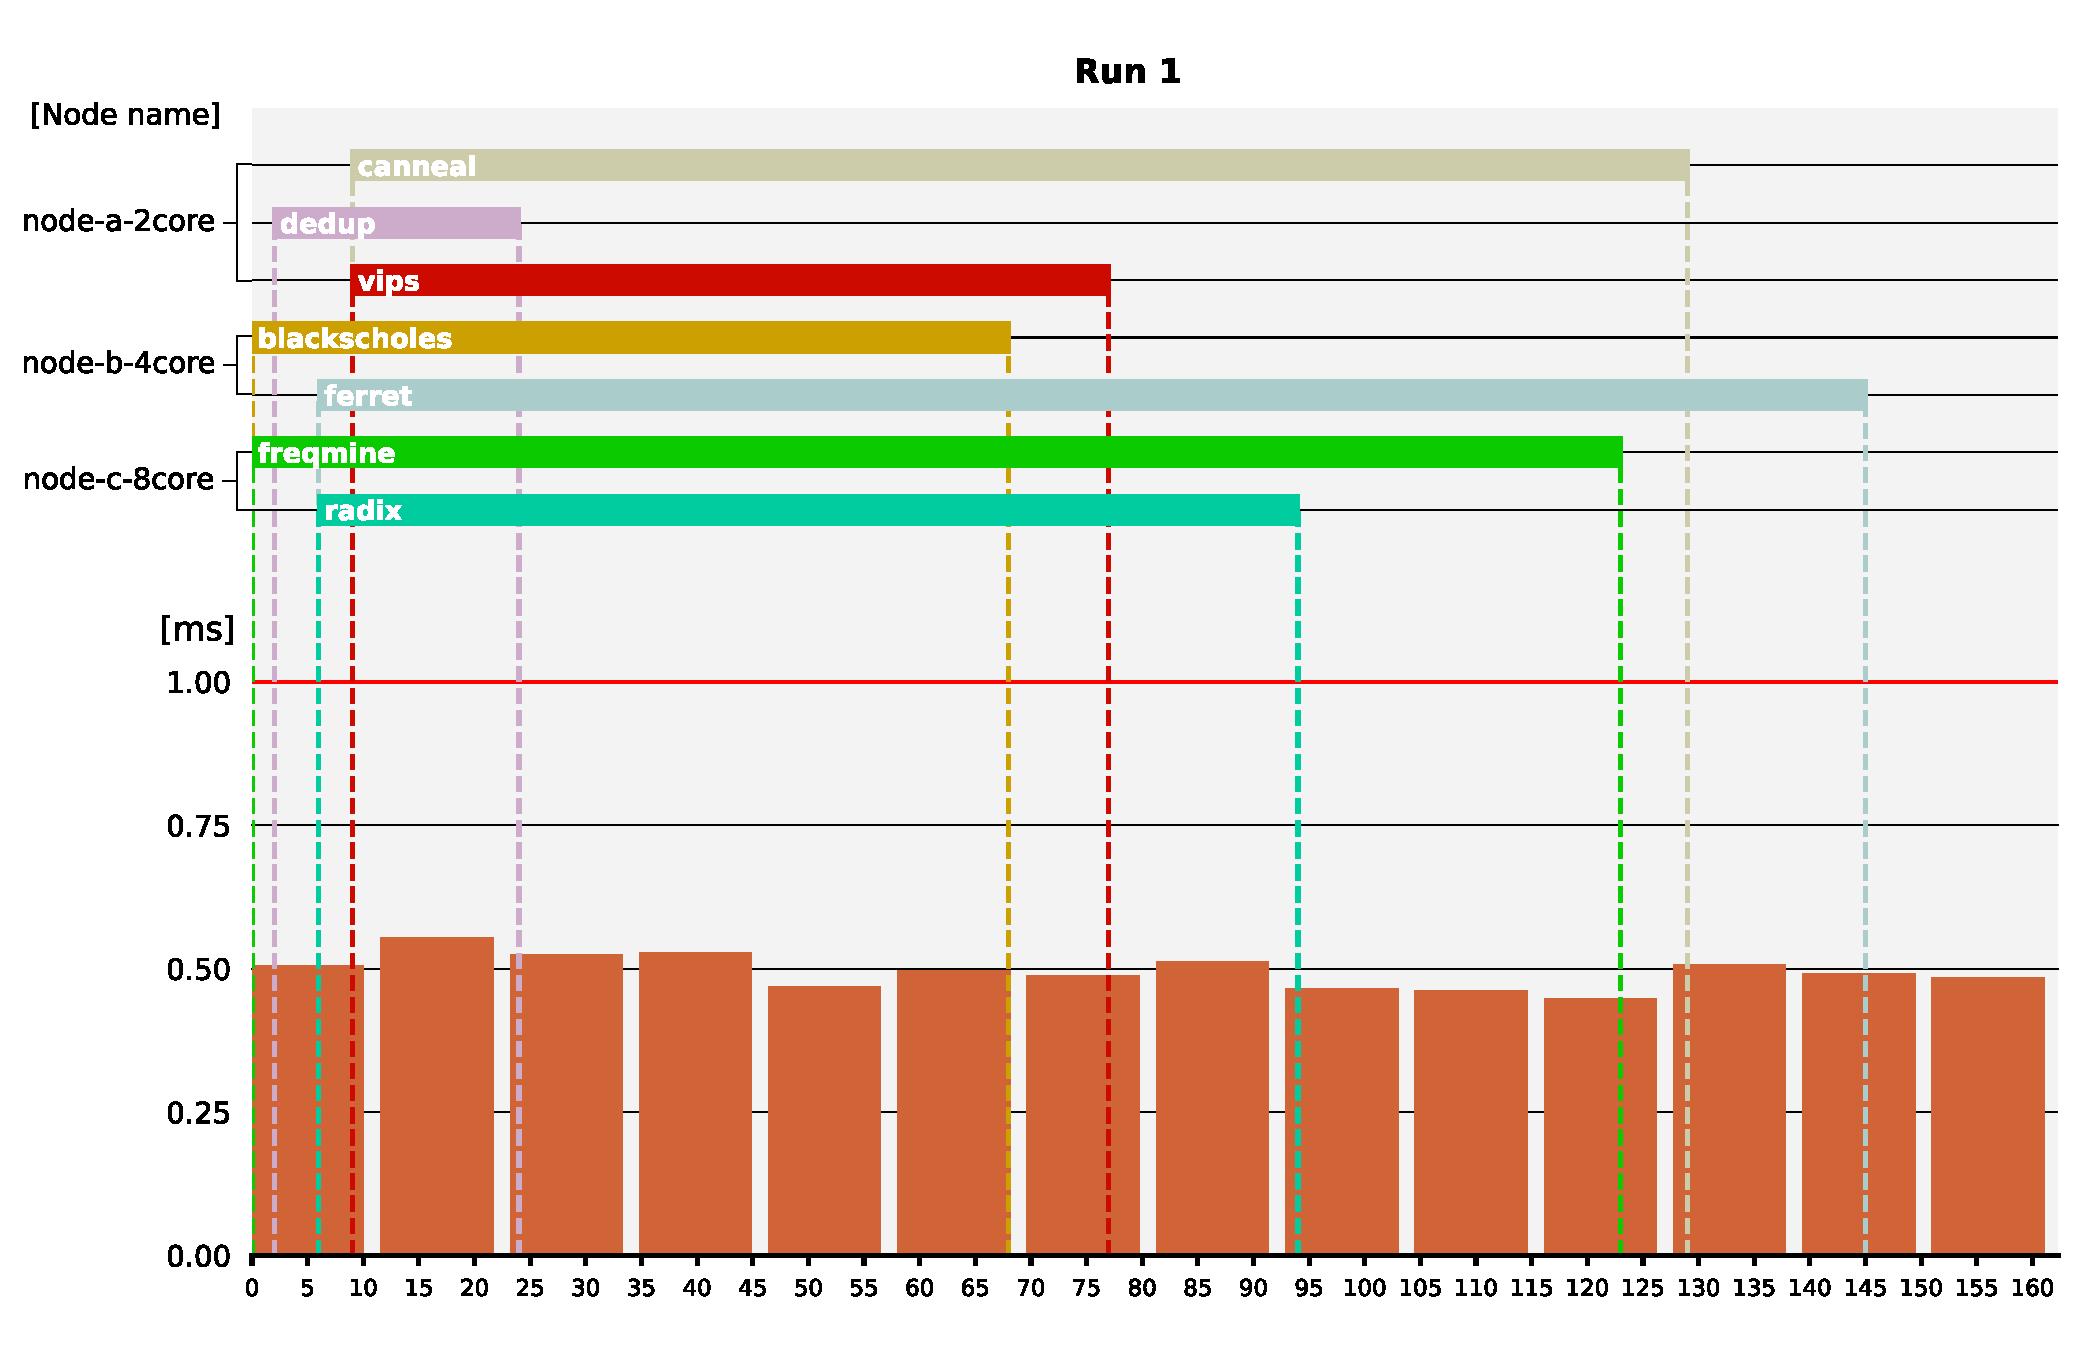
\includegraphics[width=.9\linewidth]{figures/part3/plot3_run_1}
        \caption{Run 1}
        \label{fig:plot3_run_1}
    \end{figure}

    \begin{figure}[htbp]
        \centering
        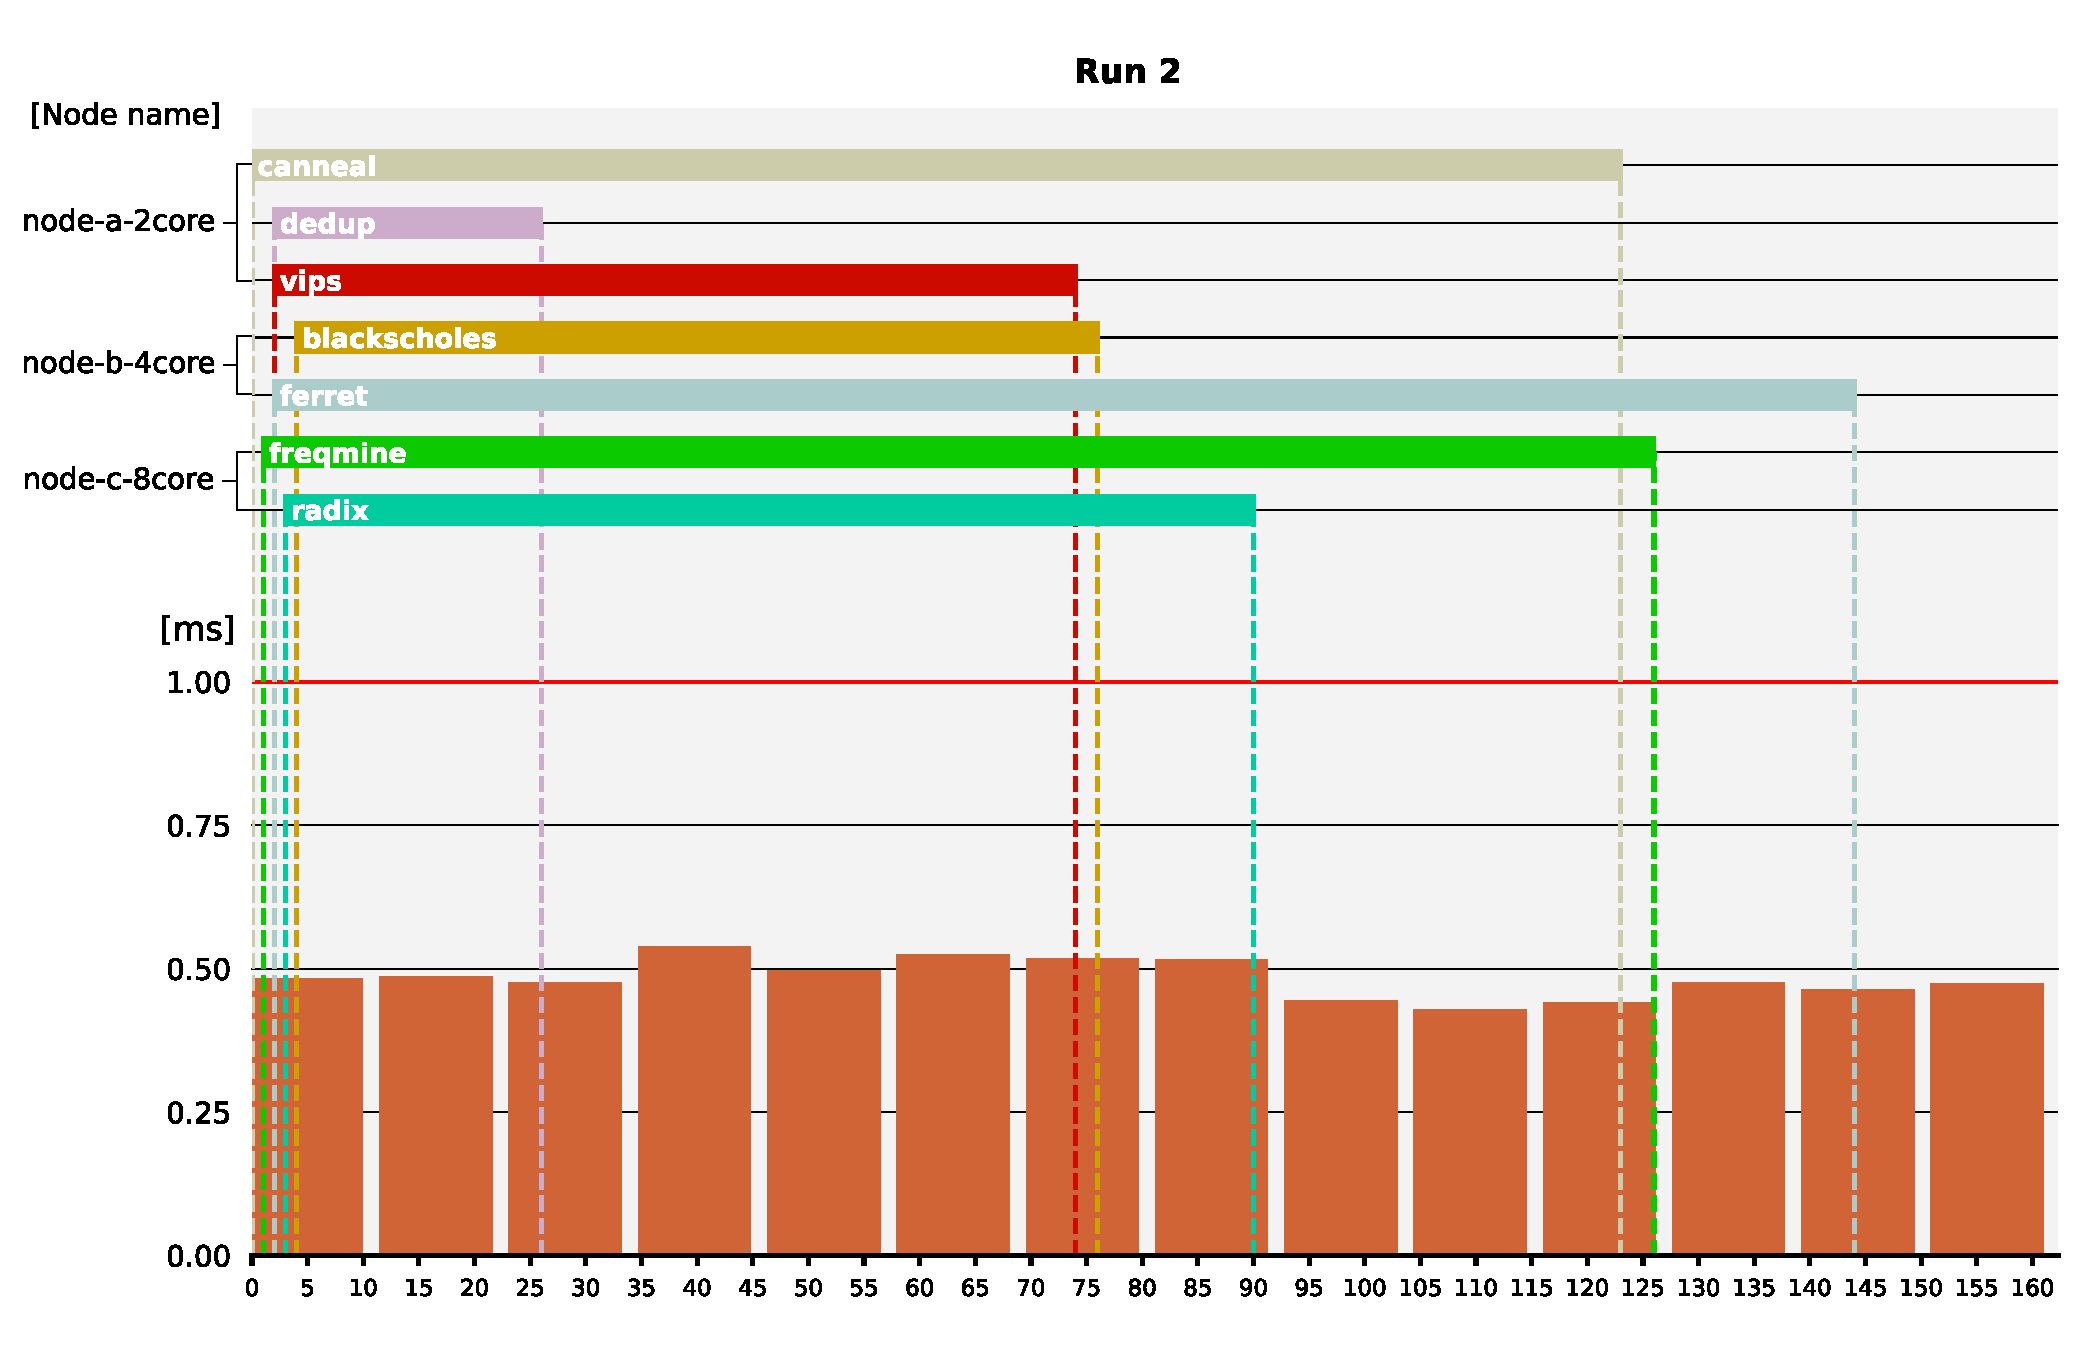
\includegraphics[width=.9\linewidth]{figures/part3/plot3_run_2}
        \caption{Run 2}
        \label{fig:plot3_run_2}
    \end{figure}

    \begin{figure}[htbp]
        \centering
        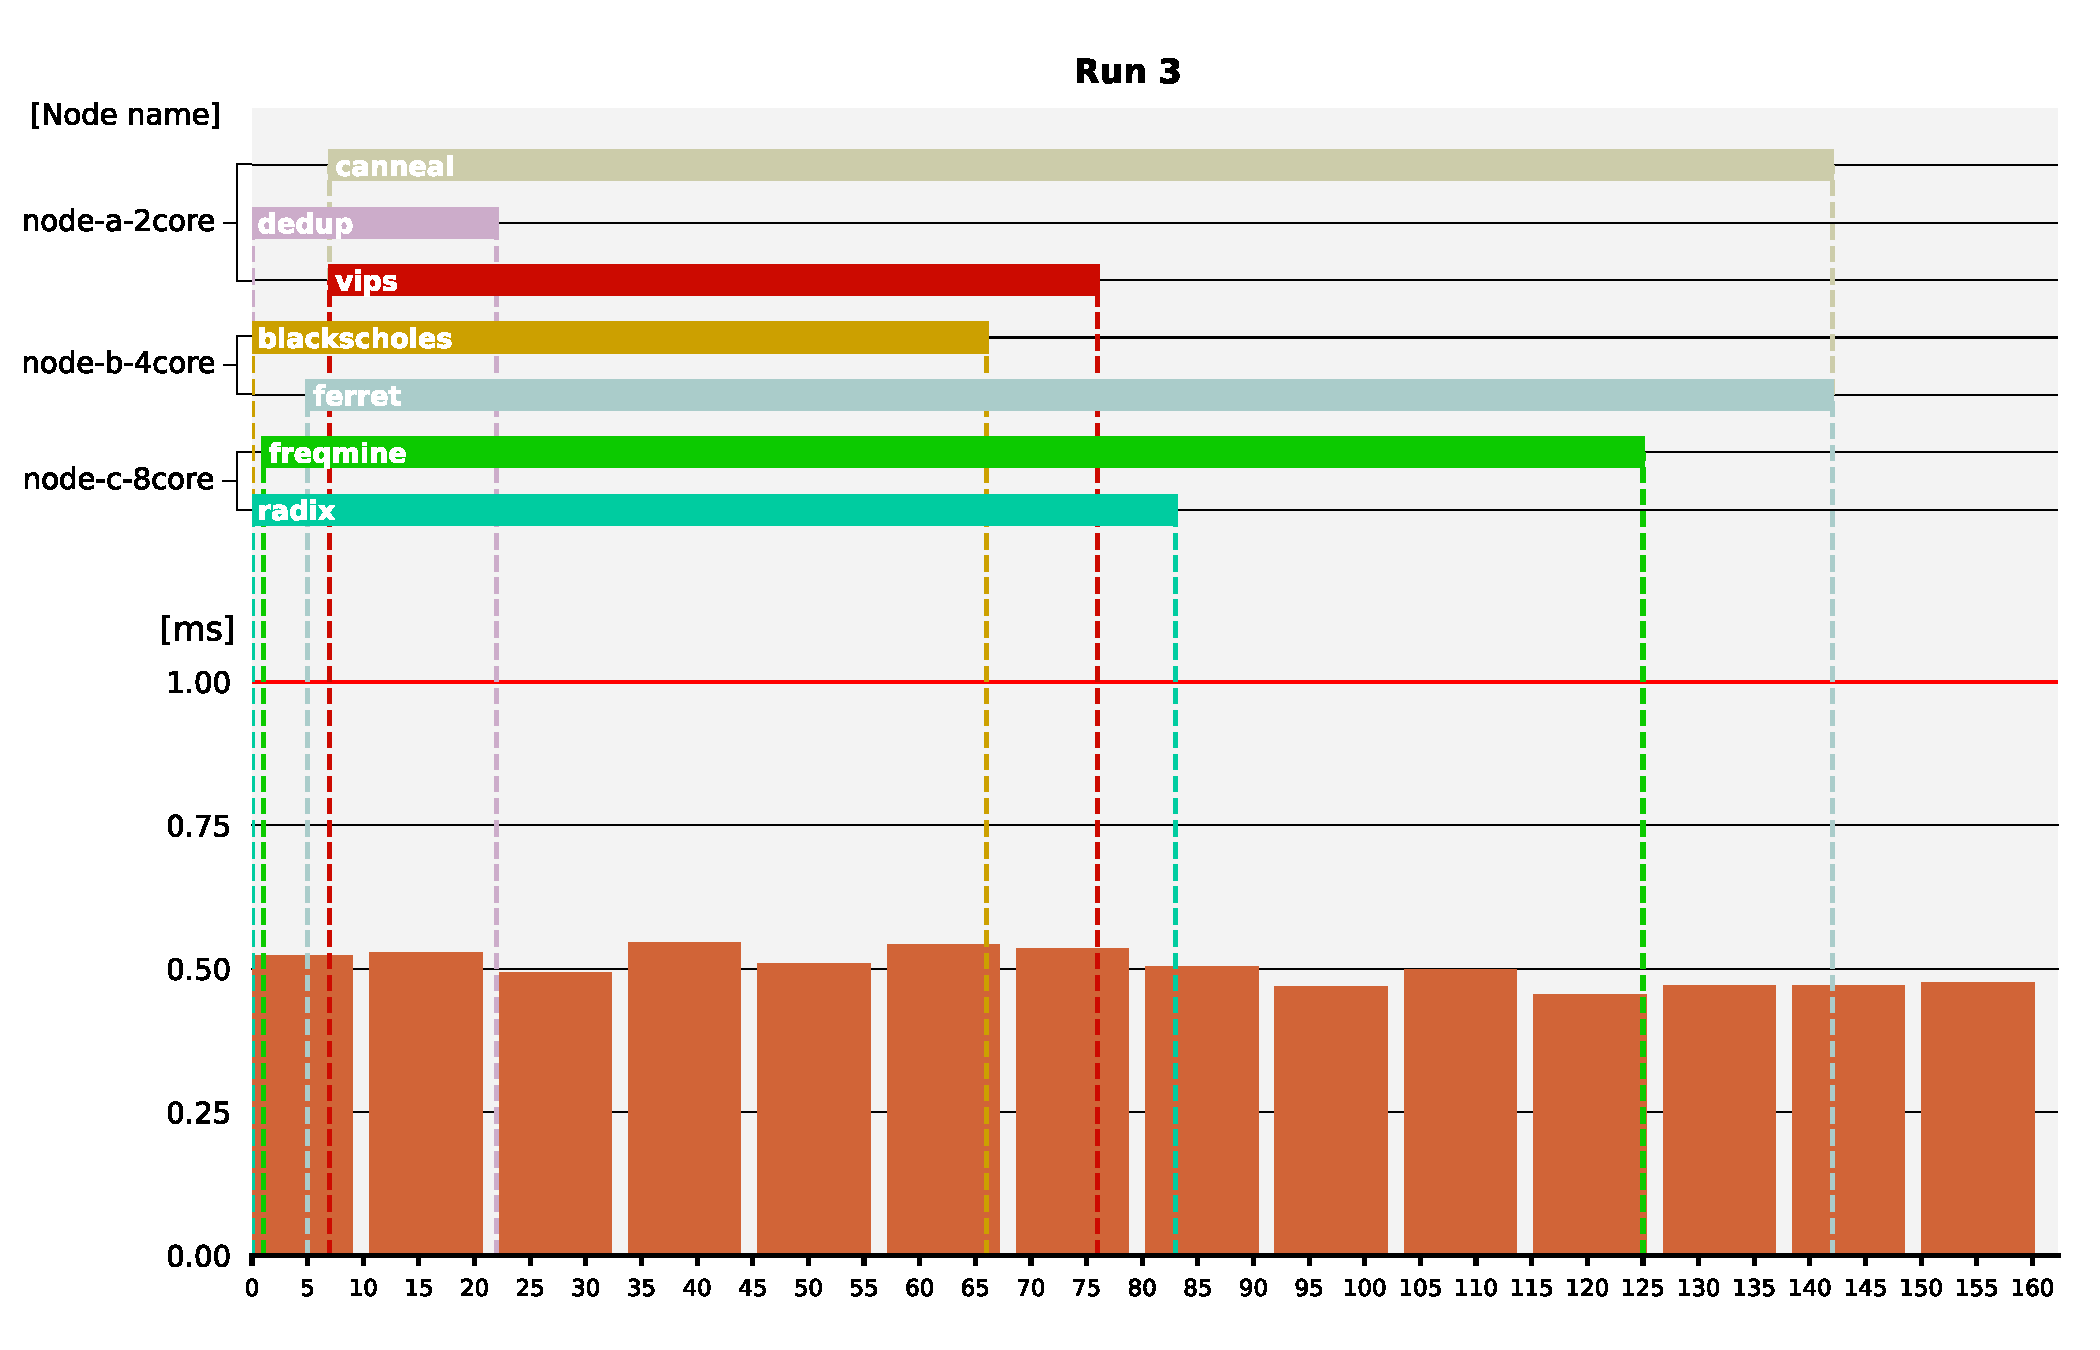
\includegraphics[width=.9\linewidth]{figures/part3/plot3_run_3}
        \caption{Run 3}
        \label{fig:plot3_run_3}
    \end{figure}

    \FloatBarrier
    
    \item \textbf{[17 points]} Describe and justify the “optimal” scheduling policy you have designed. 
    
    \begin{itemize}
        \item Which node does memcached run on? Why?

        \textbf{Answer:} % Put your solution here
        Memcached is running on node-c-8core with its CPU affinity set to CPU 0. We took into account several factors while deciding the node for memcached.

        Firstly, memcached does not require much CPU and memory while operating at a constant 30K QPS. Testing it, we found out that it needs just 0.5 CPU and 32MB memory to run smoothly.
        
        Secondly, after consulting the documentation, we discovered that the e2-standard-8 machine, despite having the highest number of cores, has weaker CPUs compared to the other machines. Therefore, we decided to reserve the faster machines for Parsec jobs.
        
        We requested at least 0.5 CPU and 32 MB memory for memcached and limited  to maximum 0.75 CPU and 64 MB respectively using Kubernetes. This configuration prevented other Parsec jobs running on the same machine and same core from using all the CPUs and memory which would have resulted in a higher latency for memcached.

        \item Which node does each of the 7 PARSEC jobs run on? Why?

        \textbf{Answer:}
        \begin{itemize}
            \item \colored{blackscholes}: % Put your solution here
            Node-b, because it performs good with four threads and node-b has four cores, providing a good environment for it to run efficiently. Assigning it less core while ferret is running on the same node would have resulted in a higher execution time of blackscholes and as a consequence a higher ferret execution time.
            
            \item \colored{canneal}: % Put your solution here
            Node-a, as it does not demand many resources but needs two cores to minimize its execution time.

            \item \colored{dedup}: % Put your solution here
            Node-a, despite being a very demanding job, it is quick to run and one core on Node-a can accommodate it.
            
            \item \colored{ferret}: % Put your solution here 
            Node-b, as it's high in CPU demand and scales well with the available cores. It is one of the most demanding jobs CPU and memory wise, we assigned also blackscholes in this node because it is not a very demanding job and they fit togheter.

            \item \colored{freqmine}: % Put your solution here
            Node-c, as it scales well with the number of cores and the eight cores of node-c helps minimize its execution time. It is the longest job to run, so we assigned it to the node with the most cores. 
            
            \item \colored{radix}: % Put your solution here
            Node-c, as it has the least resource requirements, and just one of the low performing cores in node-c is sufficient for it. Being very low demanding do not interfere much with freqmine neither interfere at all with memcached.

            \item \colored{vips}: % Put your solution here
            Node-a, because it requires high memory transfer speed which node-a provides being the best spec machine amongst all.
            
        \end{itemize}

        Further explanation on our motivations is given in the section regarding design choices at the end of Part 3.

        \item Which jobs run concurrently / are colocated? Why?

        \textbf{Answer:} % Put your solution here
        On node-a, canneal, dedup, and vips are run concurrently because it minimizes the total execution time compared to running them sequentially.
        
        On node-b, blackscholes and ferret are run concurrently. Even though ferret's execution time increases by 20\% when colocated with blackscholes, the total time for running both is less than running them separately.
        
        On node-c, freqmine and radix are run concurrently. Radix shares the core with the memcached server because it has low resource needs and doesn't interfere with the server's performance.

        \item In which order did you run 7 PARSEC jobs? Why?
    
        \textbf{Order}: % Sort them 
        \colored{blackscholes}, \colored{canneal}, \colored{dedup}, \colored{ferret}, \colored{freqmine}, \colored{radix}, \colored{vips}
    
    
        \textbf{Why}: % Put your solution here
        All the jobs are started \textbf{concurrently} on the three nodes, hence there is no order in which they are started.

        \item How many threads have you used for each of the 7 PARSEC jobs? Why?
    
        \textbf{Answer:}
    
        \begin{itemize}
            \item \colored{blackscholes}: % Put your solution here
            Four threads because it performs better with four threads and 4 cores. Assigning it less threads would have increased its execution time exceeding the achieved runtime. Using two cores has been tested but it is not as efficient as using four cores because it takes long to complete and interfere longer with ferret that is a demanding job running on the same node.

            \item \colored{canneal}: % Put your solution here
            Two threads as it is run on node-a which has two cores, and this minimizes its execution time. Using more thread is not beneficial as it doesn't scale well with more than two thread.

            \item \colored{dedup}: % Put your solution here
            One thread, as it runs on one core of node-a and completes quickly. Moreover it doesn't scale well with more threads. Just one core was assigned also to interfere less with canneal that is running on the same node.

            \item \colored{ferret}: % Put your solution here 
            Four threads, as it is run on node-b, which has four cores, and it scales well with more cores.

            \item \colored{freqmine}: % Put your solution here
            Eight threads because it is run on node-c which has eight cores and it scales well with the number of cores. Using four threads would have increased its execution time significantly.

            \item \colored{radix}: % Put your solution here
            One thread because it has low resource requirements and shares a core with the memcached server on node-c. It is actually run with just 0.1 CPU and a hard limit on 0.25 to not interfere with the memcached server. It does not interfere also with freqmine that is a demanding job running on the same node.

            \item \colored{vips}: % Put your solution here
            One thread because it is quick to run and it can share the core only with canneal, using two cores would mean share the core with three process concurrently. It is assigned in the other core respect to dedup, so they do not interfere with each other ends quickly and leave the resources to canneal.
        \end{itemize}



        \item Which files did you modify or add and in what way? Which Kubernetes features did you use?
    
        \textbf{Answer:} % Put your solution here
        We revised seven YAML configuration files corresponding to the seven PARSEC jobs. The modifications involved setting the number of threads each job should use, defining the CPU affinity via the \texttt{taskset} command and the \texttt{nodeSelector} property to specify on which node each job should run.
        
        Additionally, the YAML configuration file for the memcached server was adjusted to specify the resource request using Kubernetes feature \texttt{Resources} using both \texttt{Request} and \texttt{limit} to set how much CPU and memory a job is assured to use and the maximum it can use respectively.
        
        A Python script was developed to automate the process of job creation, memcached server setup, and the implementation of the scheduling mechanism. Find below the output of the help command of this script which describes the different functionalities it provides.

        % TODO: Maybe we can include the output of the help command as it is really well done

        \begin{verbatim}
python3 main.py --help
usage: main [-h] {create,status,start,stop,destroy,ssh,test,time} ...

Command line interface for cluster operations

positional arguments:
{create,status,start,stop,destroy,ssh,test,time}
    create              create cluster
    status              get status
    start               start service
    stop                stop service
    destroy             destroy cluster
    ssh                 ssh to a node
    test                test a scheduler
    time                analyze results

optional arguments:
-h, --help            show this help message and exit
        \end{verbatim}
        
        \vspace{1cm}

        \item Describe the design choices, ideas and trade-offs you took into account while creating your scheduler (if not already mentioned above):

        \textbf{Answer:} % Put your solution here
        The main design consideration for the scheduler was to minimize total execution time of all jobs, while not interfering much with the memcached execution. This was achieved by:
        \begin{itemize}
            \item Co-locating jobs that are compatible in terms of resource usage. For instance, ferret and blackscholes are run together on node-b, while canneal, dedup, and vips are colocate on node-a.
            \item Matching jobs with the right nodes based on their resource demands and the node's capabilities. For example, vips is put on node-a because it requires high memory transfer speed.
            \item Running jobs concurrently on each node instead of sequentially to minimize total execution time.
            \item Adjusting the number of threads each job uses according to the number of cores in each node and the individual job's performance under various thread counts. For instance, blackscholes runs with four threads on node-b because it performs better under these conditions, while freqmine uses all eight cores of node-c because it scales well with the number of cores.

        \end{itemize}

        The major trade-off in this scheduler design is slowing down the individual execution time of each job to minimize the total execution time. For example, the execution time of ferret increases by about 20\% when run together with blackscholes on node-b, but the total execution time of both jobs is less when run together compared to running them consecutively.

        Another trade-off is the choice to limit the number of cores/threads some jobs can use despite their ability to scale well with more cores. This decision is made to ensure other processes or jobs on the same node are not negatively affected. For example, radix, despite scaling the best with the number of cores, is limited to use only 0.25 core on node-c to avoid interfering with memcached, it is still very fast to complete and it would be a waste of CPU power to assign to it more CPUs. Similarly, vips, despite scaling well, is limited to use only one core on node-a to not compete with three jobs concurrently, also it is faster than canneal to complete and therefore canneal has been assigned two cores to complete faster.

        The design of the scheduler involves a delicate balance of maximizing the utilization of available resources, managing co-locations to minimize total execution time, and respecting the specific needs and characteristics of each job. These decisions have been taken looking at the characteristics of each job and the resources available on each node, and by running experiments to determine the best number of threads for each job. We took into account also the scalability and resource demand of each jobs tested on part 2.
        
        Looking at the documentation we realize that the most powerful CPU are in node-a, following node-b and node-c so we run every job alone in every machine with various number of threads and core to find how much time each jobs takes on each configuration to be able later with all the information to decide better where and how schedule the jobs. The results of this experiment can be found in \autoref{tab:my-table}

        %TODO: include the table with the times Lorenzo did

        \begin{table}[!htp]\centering
            \caption{Runtime (s) of PARSEC jobs on various configurations} \label{tab:my-table}
            \scriptsize
           
            \begin{tabular}{ccccc}\toprule
            \multicolumn{4}{c}{\textbf{Blackscholes}} \\
            \midrule
            Number of cores &Runtime in node-a &Runtime in node-b &Runtime in node-c \\
            \midrule
            1 &01:04 &01:33 &02:09 \\
            2 &00:37 &01:02 &01:16 \\
            4 & &00:49 &00:49 \\
            8 & & &00:38 \\
            \toprule
            \multicolumn{4}{c}{\textbf{Canneal}} \\
            \midrule
            Number of cores &Runtime in node-a &Runtime in node-b &Runtime in node-c \\
            \midrule
            1 &02:32 &03:16 &05:06 \\
            2 &01:32 &02:05 &03:10 \\
            4 & &01:32 &02:05 \\
            8 & & &01:40 \\
            \toprule
            \multicolumn{4}{c}{\textbf{Dedup}} \\
            \midrule
            Number of cores &Runtime in node-a &Runtime in node-b &Runtime in node-c \\
            \midrule
            1 &00:19 &00:25 &00:39 \\
            2 &00:17 &00:24 &00:19 \\
            4 & &00:24 &00:15 \\
            8 & & &00:15 \\
            \toprule
            \multicolumn{4}{c}{\textbf{Vips}} \\
            \midrule
            Number of cores &Runtime in node-a &Runtime in node-b &Runtime in node-c \\
            \midrule
            1 &01:09 &01:35 &01:42 \\
            2 &00:50 &01:05 &00:56 \\
            4 & &00:59 &00:31 \\
            8 & & &00:25 \\
            \toprule
            \multicolumn{4}{c}{\textbf{Freqmine}} \\
            \midrule
            Number of cores &Runtime in node-a &Runtime in node-b &Runtime in node-c \\
            \midrule
            1 &04:11 &05:14 &08:15 \\
            2 &02:08 &02:38 &03:40 \\
            4 & &1:50 &01:55 \\
            8 & & &01:21 \\
            \toprule
            \multicolumn{4}{c}{\textbf{Ferret}} \\
            \midrule
            Number of cores &Runtime in node-a &Runtime in node-b &Runtime in node-c \\
            \midrule
            1 &05:22 &06:46 &08:15 \\
            2 &02:44 &03:27 &04:08 \\
            4 & &02:27 &02:06 \\
            8 & & &01:46 \\
            \toprule
            \multicolumn{4}{c}{\textbf{Radix}} \\
            \midrule
            Number of cores &Runtime in node-a &Runtime in node-b &Runtime in node-c \\
            \midrule
            1 &00:31 &00:40 &00:59 \\
            2 &00:17 &00:25 &00:31 \\
            4 & &00:16 &00:16 \\
            8 & & &00:16 \\
            \bottomrule
            \end{tabular}
            \end{table}
        
    \end{itemize}
\end{enumerate}

\newpage

\section*{Part 4 [76 points]}

\begin{enumerate}
\itemsep 2em
    
    \item \textbf{[20 points]} Use the following \texttt{mcperf} command to vary QPS from 5K to 125K in order to answer the following questions: 
    \begin{Verbatim}[fontsize=\small]
$ ./mcperf -s INTERNAL_MEMCACHED_IP --loadonly 
$ ./mcperf -s INTERNAL_MEMCACHED_IP -a INTERNAL_AGENT_IP  \
           --noload -T 16 -C 4 -D 4 -Q 1000 -c 4 -t 5 \ 
           --scan 5000:125000:5000
    \end{Verbatim}

    a) [10 points] How does memcached performance vary with the number of threads ($T$) and number of cores ($C$) allocated to the job? In a single graph, plot the 95th percentile latency (y-axis) vs. QPS (x-axis) of memcached (running alone, with no other jobs collocated on the server) for the following configurations (one line each):
    \begin{itemize}
        \item Memcached with $T$=1 thread, $C$=1 core
        \item Memcached with $T$=1 thread, $C$=2 cores
        \item Memcached with $T$=2 threads, $C$=1 core
        \item Memcached with $T$=2 threads, $C$=2 cores
    \end{itemize}
    
    Label the axes in your plot. State how many runs you averaged across (we recommend three runs) and include error bars. The readability of your plot will be part of your grade.
    
    \textbf{Plots:} % Put your plots here

    % Plot plot1_1.pdf is the plot for T=1, C=1
    \begin{figure}[htbp]
        \centering
        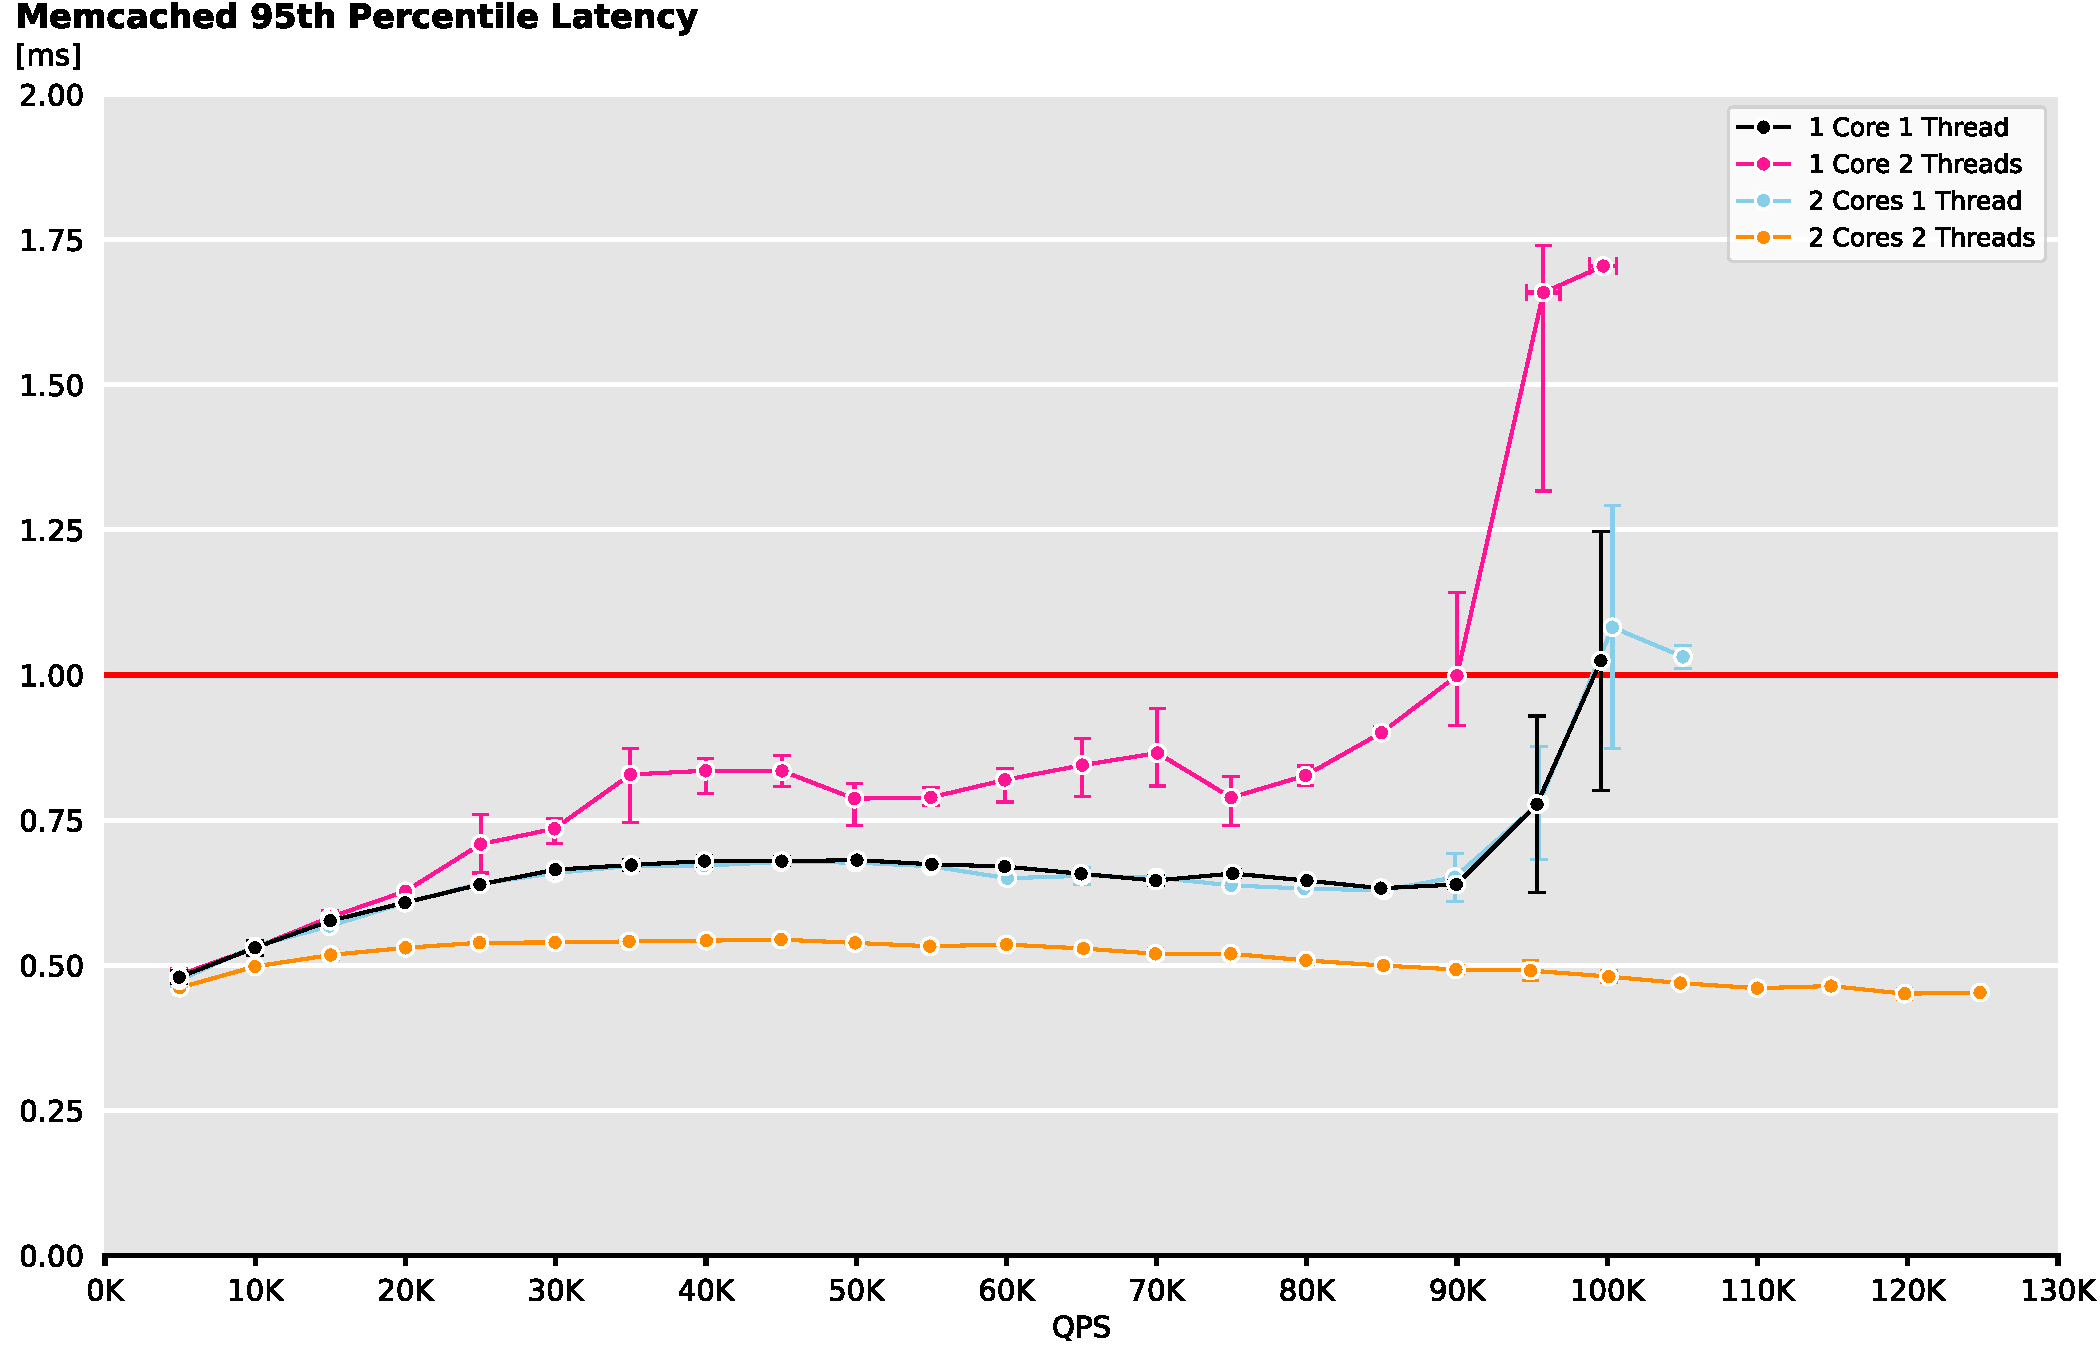
\includegraphics[width=0.8\textwidth]{figures/part4/plot1_1.pdf}
        \caption{95th percentile latency vs. QPS for memcached avaraged over 3 runs}
        \label{fig:part4_plot1_1}
    \end{figure}

    Error bars are present in all plots, but some measurement were too consistent and the error is too little to be visible on some part of the graph. 105K QPS in 2 core 1 thread is reached just one time out of 3 runs, we reported it for completeness.
    
    What do you conclude from the results in your plot? Summarize in 2-3 brief sentences how memcached performance varies with the number of threads and cores.
    
    \textbf{Summary:} The results indicate that memcached performance is least efficient with 1 core and 2 threads, likely due to the overhead of managing an extra thread on a single core and due to the threads competing with each other to use the core. Maximum performance is observed with a configuration of 2 cores and 2 threads, which allows the threads to operate in parallel. Other configurations, specifically 2 cores with 1 thread, yield similar performance to a 1 core 1 thread setup, due to the singular thread being confined to one core.
    
    % The worst performing configuration is clearly 1 core 2 threads. This is due to the overhead of having an additional thread when only one core is available. The best performing configuration is 2 cores 2 threads. This is due to the fact that the threads can be scheduled on different cores, and thus the threads can run in parallel. The other two configurations are in between these two extremes, with really similar performance. This is due to the fact that with 2 cores but only 1 thread the thread will be scheduled exclusively on one core, and thus the performance is similar to the 1 core 1 thread configuration.    
    
    b) [2 points] To support the highest load in the trace (125K QPS) without violating the 1ms latency SLO, how many memcached threads ($T$) and CPU cores ($C$) will you need?
    
    \textbf{Answer:} From the plot it is clearly visible that the only configuration that did not violate the SLO at 125K QPS was 2 Cores 2 Threads. Therefore, we will need 2 Cores and 2 Threads to support the highest load in the trace without violating the 1ms latency SLO.
    
    c) [1 point] Assume you can change the number of cores allocated to memcached dynamically as the QPS varies from 5K to 125K, but the number of threads is fixed when you launch the memcached job. How many memcached threads ($T$) do you propose to use to guarantee the 1ms 95th percentile latency SLO while the load varies between 5K to 125K QPS?
    
    \textbf{Answer:} If you can change the number of cores allocated to memcached dynamically as the QPS varies from 5K to 125K, but the number of threads is fixed when you launch the memcached job, then you should use 2 memcached threads ($T$) to guarantee the 1ms 95th percentile latency SLO while the load varies between 5K to 125K QPS. This is because the configuration of 2 cores and 2 threads provided the best performance in the plot and is the only one capable od handling 125K QPS, by fixing the number of threads to 2, you can ensure that the threads can be scheduled on different cores as the number of cores allocated to memcached changes dynamically. While is true that 2 cores and 1 thread is the configuration with the worst performance, in case the load becomes to high we can change to 2 cores and 2 threads to ensure that the SLO is not violated.
    
    d) [7 points] Run memcached with the number of threads $T$ that you proposed in (c) and measure performance with $C=1$ and $C=2$. Use the aforementioned \texttt{mcperf} command to sweep QPS from 5K to 125K.

    Measure the CPU utilization on the memcached server at each 5-second load time step.
    
    Plot the performance of memcached using 1-core ($C=1$) and using 2 cores ($C=2$) in \textbf{two separate graphs}, for $C=1$ and $C=2$,  respectively. In each graph, plot QPS on the x-axis, ranging from 0 to 130K. In each graph, use two y-axes. Plot the 95th percentile latency on the left y-axis. Draw a dotted horizontal line at the 1ms latency SLO. Plot the CPU utilization (ranging from 0\% to 100\% for $C=1$ or 200\% for $C=2$) on the right y-axis. For simplicity, we do not require error bars for these plots. 
    
    \textbf{Plots:} % Put your plots here
    
    \begin{figure}[htbp]
        \centering
        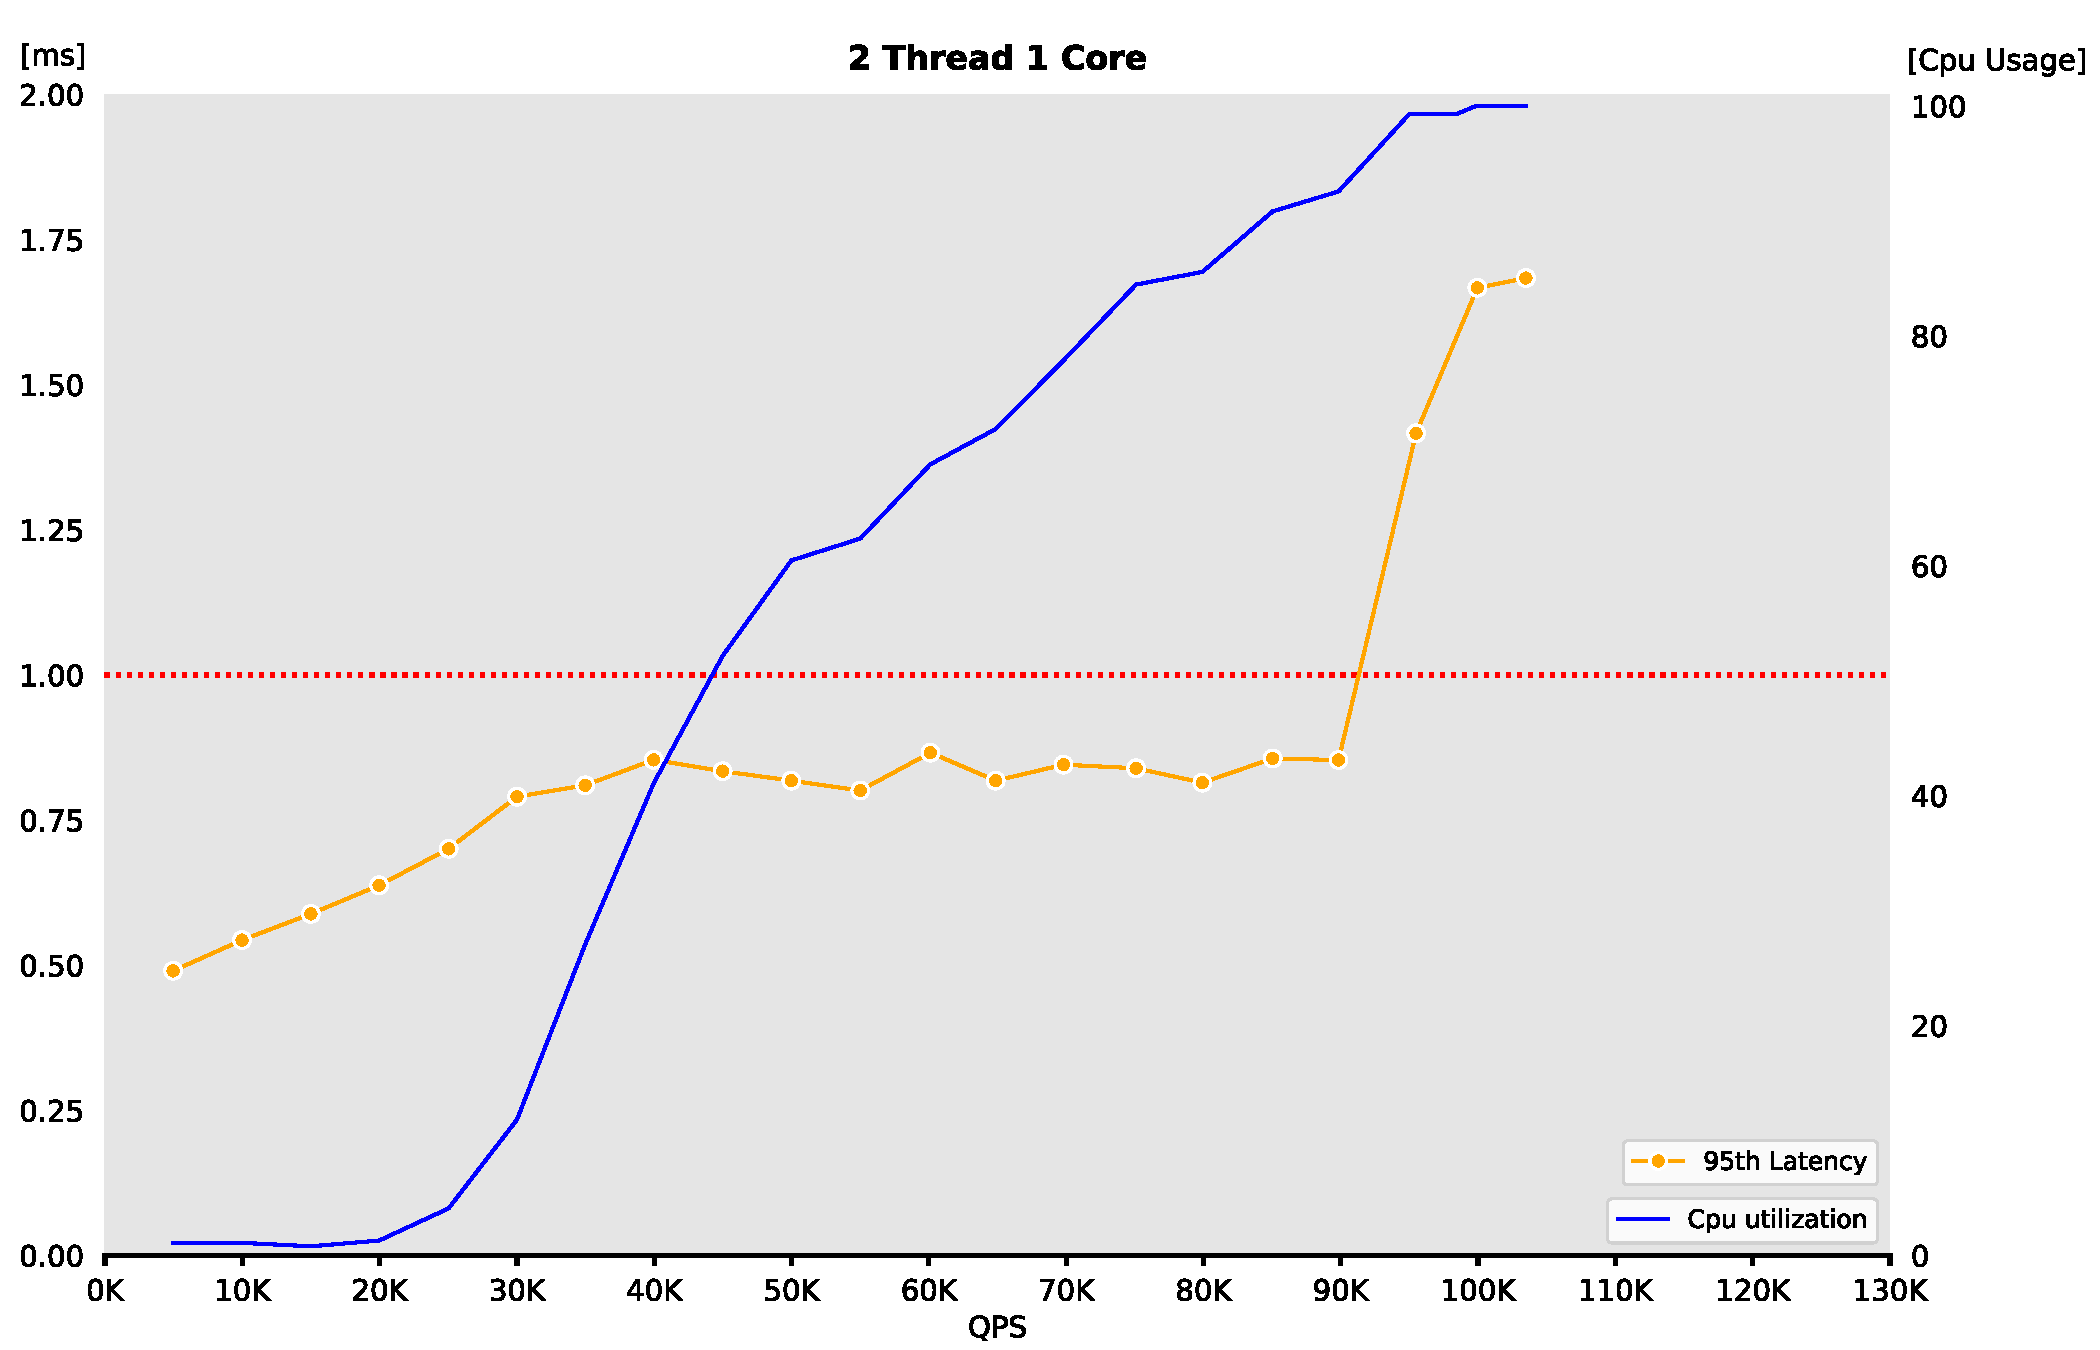
\includegraphics[width=0.8\textwidth]{figures/part4/plot1_1_1.pdf}
        \caption{95th percentile latency vs. QPS for memcached with 1 core}
    \label{fig:part4_plot1_2}
    \end{figure}

    \begin{figure}[htbp]
        \centering
        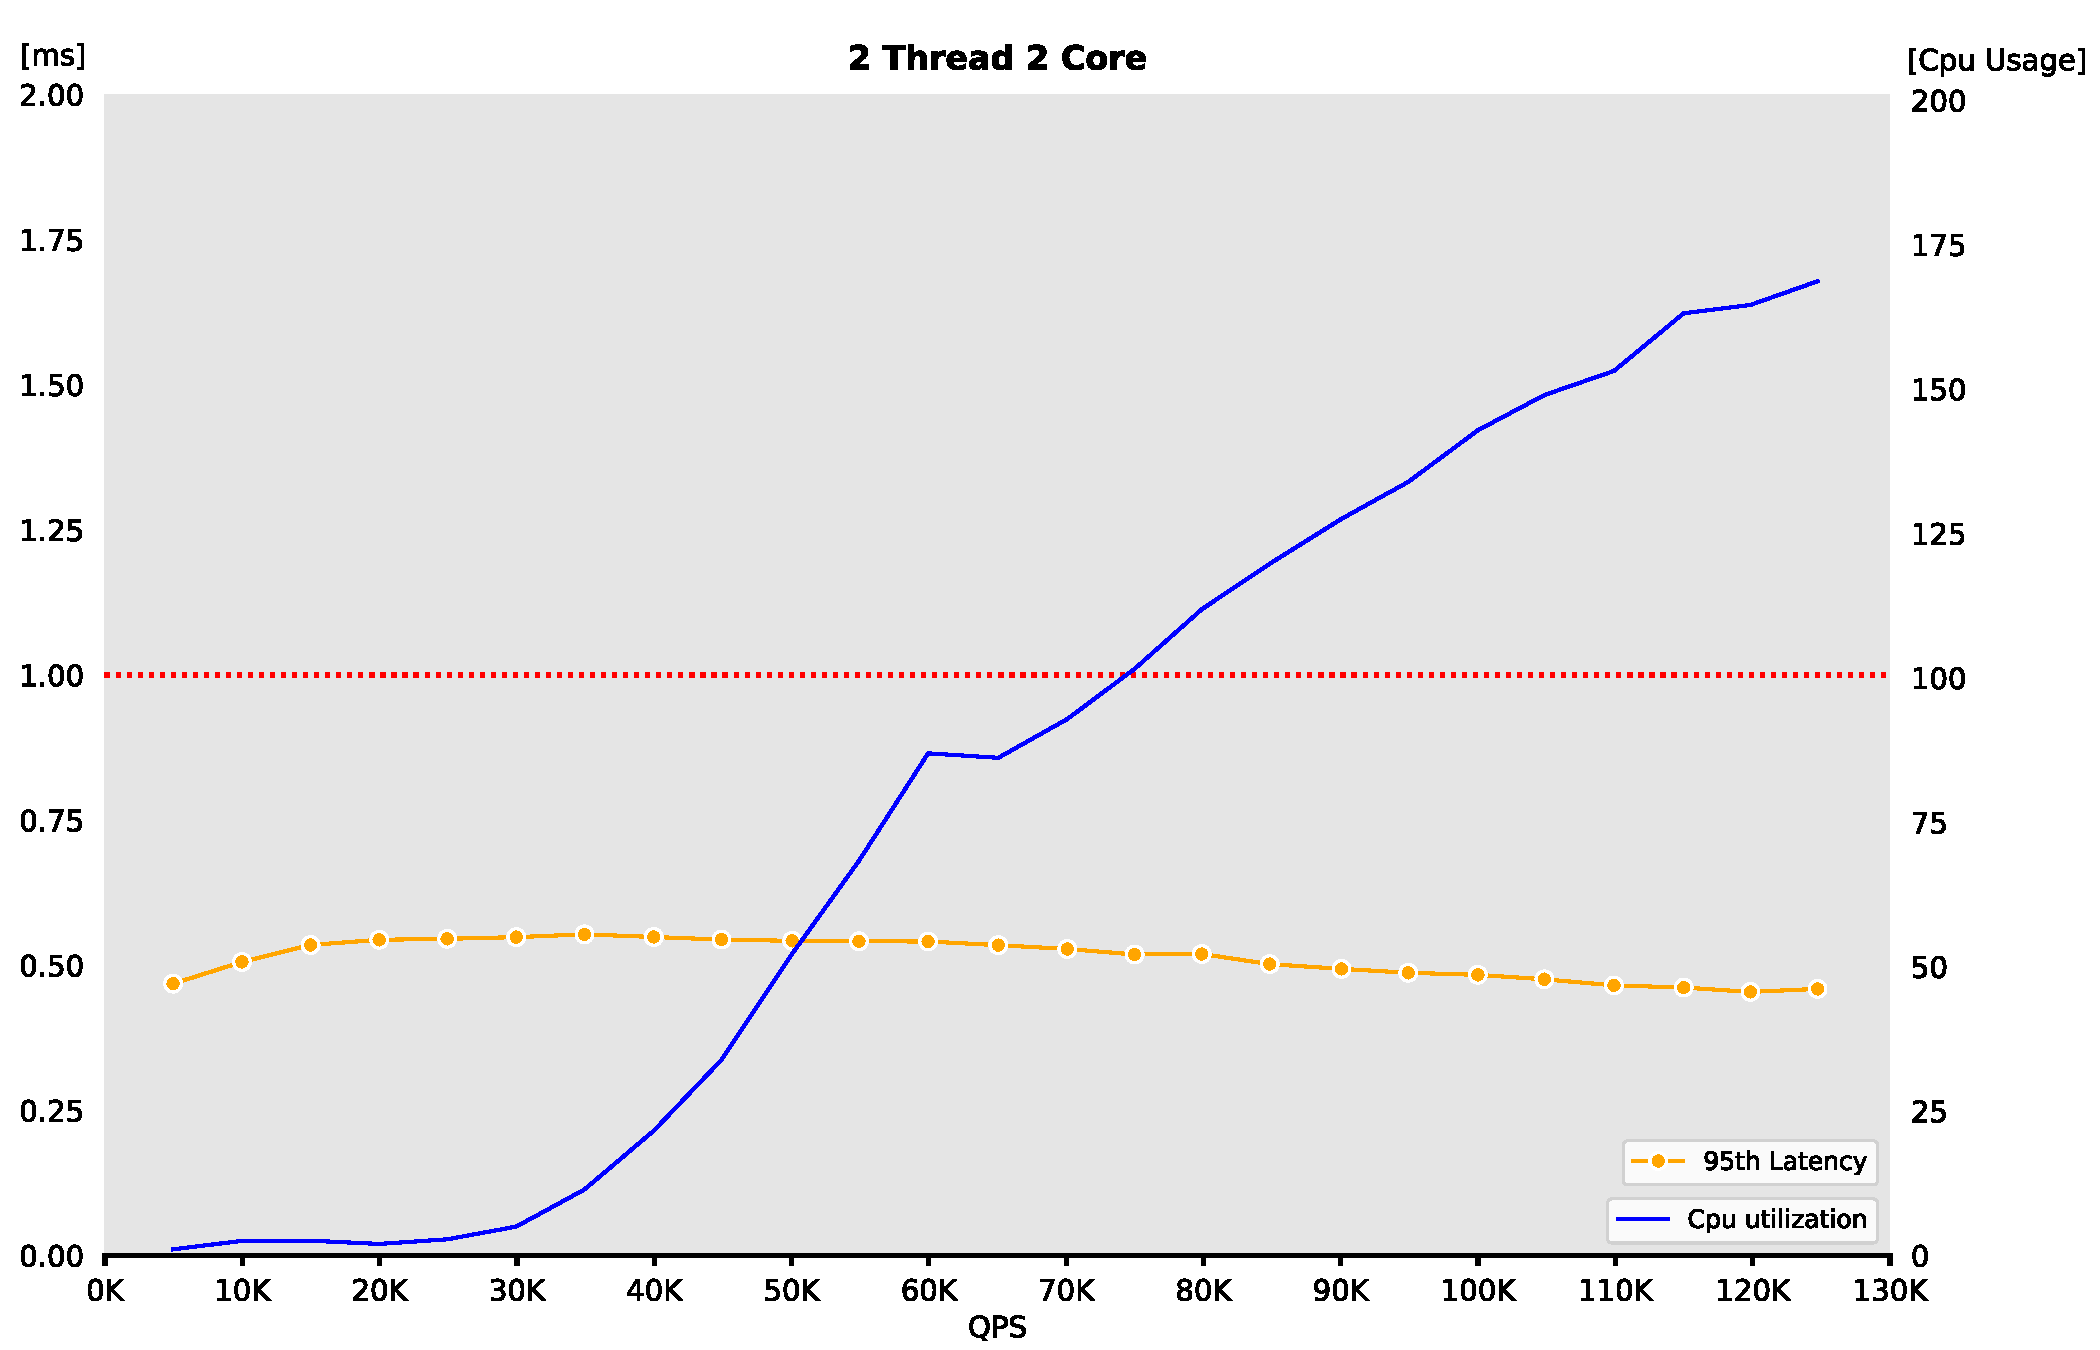
\includegraphics[width=0.8\textwidth]{figures/part4/plot1_1_2.pdf}
        \caption{95th percentile latency vs. QPS for memcached with 2 cores}
    \label{fig:part4_plot1_3}
    \end{figure}

    % new page
    \newpage
    
    \item \textbf{[17 points]} You are now given a dynamic load trace for memcached, which varies QPS randomly between 5K and 100K in 10 second time intervals. Use the following command to run this trace: 
        \begin{Verbatim}[fontsize=\small]
$ ./mcperf -s INTERNAL_MEMCACHED_IP --loadonly 
$ ./mcperf -s INTERNAL_MEMCACHED_IP -a INTERNAL_AGENT_IP \ 
           --noload -T 16 -C 4 -D 4 -Q 1000 -c 4 -t 1800 \ 
           --qps_interval 10 --qps_min 5000 --qps_max 100000
\end{Verbatim}
    
    Note that you can also specify a random seed in this command using the \texttt{--qps\_seed} flag. 

    For this and the next questions, feel free to reduce the mcperf measurement duration (\texttt{-t} parameter, now fixed to 30 minutes) as long as you have at the end at least 1 minute of memcached running alone.
    
    Design and implement a controller to schedule memcached and the PARSEC benchmarks on the 4-core VM. The goal of your scheduling policy is to successfully complete all PARSEC jobs as soon as possible without violating the 1ms 95th percentile latency for memcached. \textbf{Your controller should not assume prior knowledge of the dynamic load trace. You should design your policy to work well regardless of the random seed.} The PARSEC jobs need to use the native dataset, i.e., provide the option \texttt{-i native} when running them. Also make sure to check that all the PARSEC jobs complete successfully and do not crash. Note that PARSEC jobs may fail if given insufficient resources.
    
    Describe how you designed and implemented your scheduling policy. Include the source code of your controller in the zip file you submit. 

    \begin{itemize}
        \item Brief overview of the scheduling policy (max 10 lines):
        
    \textbf{Answer:} The scheduling policy manages CPU resources between memcached and the PARSEC benchmark jobs using Docker containers. Two job queues handle single-core and dual-core jobs. The policy keeps a check on CPU usage and adjusts memcached's CPU affinity as required. Memcached primarily operates on core 0, occasionally utilizing core 1 based on load. High CPU usage triggers a pause on the core 1 job, allocating its CPU to memcached. Low usage lets the paused job resume or starts a new one, confining memcached to core 0. High CPU usage is defined as above 80\% on a single core or less than 130\% combined on two cores. The policy assigns core 1 to canneal, vips, blackscholes, and dedup, while cores 2 and 3 are allocated to ferret, freqmine, and radix. After radix, ferret and freqmine complete, other jobs can also utilize cores 2 and 3.

     % Put your solution here
    % The policy is designed to ensure that the memcached process is allocated the appropriate number of CPU cores based on the CPU utilization of the system, while also ensuring that the PARSEC benchmark jobs are allocated the appropriate number of CPU cores and threads based on their resource requirements and the CPU utilization of the system. The policy is implemented using a combination of if-else statements and while loops to continuously monitor the system and adjust the resource allocation of the Docker containers and memcached process as needed.

    % The program uses two queues, one for jobs that require one core and another for jobs that require two cores. The program starts by creating Docker containers for each job and adding them to the appropriate queue. The program then continuously checks the CPU utilization and adjusts the CPU affinity of the memcached process accordingly. memcached can run in cores 0 and 1, depending on the load. If the CPU utilization is high, the program pauses any running job in core 1 and allocates its CPU core to memcached. If the CPU utilization is low, the program resumes the paused job or starts a new job if there are no paused jobs, and removes memcached from core 1 reserving core 0 exclusively. The program ends when all jobs have completed successfully and memcached has run for 60 seconds afterwards.

    % CPU utilization is only measured for the cores where memcached is running. It is considered high if it is greater than 80% when it is running only one core one core and if the sum of the CPU utilization of the two cores is less than 130% when two cores are scheduled.

    % The program allocates sequentially core 1 to each of the following jobs: canneal, vips, blackscholes, and dedup. The program allocates cores 2 and 3 exlusively and sequentially to each of the following jobs: ferret, and freqmine.

    % In case both ferret and freqmine have finished, the other jobs that tun exclusisvely on core 1 are allowed to run on core 2 and 3 as well.
    % The scheduling policy focuses on managing the CPU resources for the memcached process and the PARSEC benchmark jobs. Using conditions and loops, the policy continuously checks the system and adjusts resource allocation for the Docker containers and memcached as needed.

    % Two job queues are used: one for single-core jobs and another for dual-core jobs. Docker containers are created for each job and added to the right queue. The policy then monitors CPU usage, adjusting the memcached process's CPU affinity accordingly.

    % Memcached runs on core 0 and sometimes on core 1, depending on the load. When the CPU usage is high, the policy pauses the job running on core 1, giving its CPU core to memcached. When the CPU usage is low, the paused job is resumed or a new job is started, and memcached is restricted to core 0. The policy ends when all jobs have finished, and memcached has run for an additional 60 seconds.

    % CPU usage is only measured on the cores running memcached. It's considered high if it's more than 80% on one core or the combined usage of two cores is less than 130%.

    % The policy sequentially assigns core 1 to canneal, vips, blackscholes, and dedup jobs, while cores 2 and 3 are exclusively and sequentially allocated to ferret, freqmine, adn radix.

    % Once ferret and freqmine finish, the other jobs initially set to run only on core 1 are allowed to use cores 2 and 3 as well.
    
    \item How do you decide how many cores to dynamically assign to memcached? Why?
    
    
    \textbf{Answer:}
     Memcached starts running on only one core. The policy assigns two cores to it when the CPU utilization is over 80\% When the CPU is less than 130\% when summing both the utilization of core 0 and 1, memcached is scaled back down to core 0.
 
     We decided to use this value as a threshold after seeing the results from the combined measure of latency and CPU using 2 threads of the previous point. We observed that until 80\% of CPU utilization, the latency was not affected. However, after that point, the latency started to increase and we need to switch.

     Additionally the 130\% worked well, because we noticed that when splitting the load between 2 processors the load on each processor did not exactly halved. Rather, it was higher than expected. Thus the combined load was set to a combined 130\% because after fusing the load of the two processors into one, the load was typically around 70\% and not maxed at 100\% as would be expected from putting together a combined load of 130\%. This behavior may be due to the fact that the operating system's scheduling mechanism may lead to uneven distribution of load, creating an imbalance in CPU usage. Imperfectly balanced threads and additional overheads from multithreading could consume more CPU time.
 
     This strategy is designed with the aim of optimizing resource use while ensuring smooth operations and effective system performance. When the system is under high load (CPU utilization above 80\%), assigning an extra core to memcached helps to improve its performance by allowing it to process more data concurrently assuring the SLO of 1ms 95th percentile latency is not violated, as high CPU utilization correlates to the number of QPS that memcached is receiving.
     
     Conversely, when the CPU utilization is relatively low (combined utilization of both cores less than 130\%), it is more efficient to limit memcached to a single core, freeing up resources for other processes or jobs that might require them, reducing the overall time of execution of the PARSEC jobs. This dynamic and responsive approach ensures a balanced, efficient use of system resources. 

    \item How do you decide how many cores to assign each PARSEC job? Why?

     \textbf{Answer:}

     \begin{itemize}
        \item \colored{blackscholes}: This job is assigned to core 1 sequentially following the scheduling policy, given that although it can benefit from parallelism its execution time is not one of the longest.
        
        \item \colored{canneal}: Similar to blackscholes, this job is also assigned to core 1 in sequence. According to the analysis in Part 1-2 Canneal is not a CPU-intensive task and it is also not one of the longest jobs. Therefore, it is not necessary to assign more than one core to it.
        
        \item \colored{dedup}: Dedup, too, is allocated to core 1 sequentially. This job is not very CPU-intensive, and also does not benefit from parallelism as much as other jobs. Moreover it is a very fast job.
    
        \item \colored{ferret}: Ferret is assigned to cores 2 and 3 exclusively, according to the policy. As a parallel search engine, ferret is a CPU-intensive task that benefits from multiple cores to improve its parallel execution. 
        
        \item \colored{freqmine}: Similar to ferret, freqmine also utilizes cores 2 and 3. As an application which performs frequent itemset mining, freqmine is a computationally intensive task and thus requires multiple cores to optimize its performance. Ferret together with freqmine are the two benchmarks that take the longer to execute, therefore any improvement on these will have a big impact on the overall runtime. Therefore, two cores were assigned to both of them.
        As mentioned before, in case ferret and freqmine finished before the other jobs running in core 1, these jobs will be also allowed to use these two core, as this was a scenario that happened sometimes in out testing.

        \item \colored{radix}: Radix is assigned to cores 2 and 3, before ferret and freqmine started. Radix was observed to have a good response to parallelism and to be really fast. Additionally, ferret and freqmine run in around 10 minutes total. Thus, there was some time available once they had finished to run one of the other jobs. These times matched more closely to the execution time of radix.
        
        \item \colored{vips}: Like blackscholes, canneal, and dedup, vips is allocated to core 1 sequentially. As an image processing system, vips requires high computational resources, but according to the analysis in Part 1-2 is less intensive than ferret or freqmine and, therefore, is allocated only one core.
 
    \end{itemize}


    \item How many threads do you use for each of the PARSEC job? Why?
    
    \textbf{Answer:}
    \begin{itemize}
        \item \colored{blackscholes}: For blackscholes, we allocate only one thread as the job runs on a single core (core 1). Multiple threads wouldn't improve performance significantly and might increase overhead due to context switching.
        
        \item \colored{canneal}: As stated, one thread is provided to canneal as it is allocated a single core. More threads would increase overhead without noticeable performance gain.
        
        \item \colored{dedup}: Dedup also receives one thread, due to its allocation on a single core. Similar reasoning to canneal and blackscholes applies here.
        
        \item \colored{ferret}: Ferret, being allocated cores 2 and 3, uses two threads to fully exploit the parallel processing capacity of the two cores. This approach significantly enhances its parallel execution performance.
        
        \item \colored{freqmine}: Freqmine also uses two threads corresponding to its allocation on cores 2 and 3. This allows the job to leverage the full computational potential of the two cores, improving its performance.
        
        \item \colored{radix}: Radix follows a similar policy to freqmine, and ferret, with two threads assigned due to its allocation on two cores (core 2 and 3).
        
        \item \colored{vips}: Vips is also allocated a single core (core 1) and thus uses one thread. Similar to blackscholes, canneal, and dedup, multiple threads would not improve performance significantly and might increase overhead due to context switching.
    \end{itemize}
      
    \item Which jobs run concurrently / are collocated and on which cores? Why?

    \textbf{Answer:} No job is run concurrently with another on the same core. Instead, jobs are allocated to cores in a sequential manner to avoid resource contention and ensure optimal execution. Memcached starts on core 0 and can expand to core 1 if the CPU utilization exceeds 80\%. On core 1, jobs blackscholes, canneal, dedup, and vips run sequentially, not concurrently. These jobs are queued up for execution on core 1 in the order they're mentioned. They may, however, be temporarily paused if memcached needs to expand to core 1 due to high CPU utilization.

     Jobs ferret, freqmine, and radix are allocated cores 2 and 3 exclusively, running sequentially on these cores. Once ferret and freqmine are finished, the other jobs initially set to run only on core 1 are allowed to run on cores 2 and 3 as well.

     While some jobs can be putted together to improve the total runtime of the scheduler like we did in part 3 the overhead to pause and unpause two or more jobs on core 1 can become too much to respond quickly to the changing QPS of memcached. ferret and freqmine which run on cores 2 and 3 are not run with other jobs because this is only going to slow down the total runtime.
     
     This design is in place to avoid resource contention and ensure each job gets exclusive access to a core for a period of time. Memcached, as a critical service, gets preferential treatment, with the ability to claim an additional core if needed.
    
    \item In which order did you run the PARSEC jobs? Why?

    \textbf{Order}: % Sort them 

    \begin{itemize}
        \item Core 1: \colored{canneal}, \colored{vips}, \colored{blackscholes}, \colored{dedup}
        \item Core 2 and 3: \colored{radix}, \colored{ferret}, \colored{freqmine}
    \end{itemize}
    
    \textbf{Why:} % Put your solution here
     There is actually not a reason for this ordering as all jobs are run sequentially and, therefore, there is no contention between them.

\item How does your policy differ from the policy in Part 3? Why?

\textbf{Answer:} % Put your solution here
In Part 3, the policy did not involve dynamically adjusting the number of running jobs based on the CPU utilization of the system and neither changing the number of cores of memcached or other applications.

In contrast, the policy in Part 4 involves dynamically adjusting the number of running containers based on the CPU utilization of the system. The policy uses the psutil library to monitor the CPU utilization of the system, and pauses and unpauses containers based on the CPU utilization. If the CPU utilization is too high, some of the containers are paused to free up resources. If the CPU utilization is low, some of the paused containers are resumed to make use of the available resources.

The main reason for this difference is that the policy in Part 4 is more flexible and can adapt to changes in the CPU utilization of the system. By dynamically adjusting the number of running containers, the policy can ensure that the system is using the available resources efficiently, while also maximizing the performance of the system. In contrast, the policy in Part 3 is more static and does not adapt to changes in the CPU utilization of the system.

We also changed the policy from running all in parallel to running just two jobs in parallel in different cores due to the reduced number of total core available.

\item How did you implement your policy? e.g., docker cpu-set updates, taskset updates for memcached, pausing/unpausing containers, etc.

\textbf{Answer:} The policy implementation involves adjusting the CPU affinity of the 'memcached' process using the \texttt{taskset} command, creating and running Docker containers for PARSEC jobs with specified CPU cores, pausing and unpausing Docker containers, and updating the cores of Docker containers. The implementation also involves monitoring the CPU utilization and adjusting the CPU affinity of 'memcached' accordingly.
We created several functions to implement the policy:

\begin{itemize}
    \item The \texttt{adjust\_memcached\_resources} function uses the \texttt{subprocess} module to call \texttt{taskset} with the following parameters:
      \begin{itemize}
      \item \texttt{\-cp} followed by the CPU cores to which `memcached` should be bound, specified as a comma-separated list of integers.
      \item \texttt{memcached\_pid}, which is the process ID of the `memcached` process.
    This is used to reschedule memcached to core 0 or to core 0 and 1 depending on the load.
    \end{itemize}
      
    \item The \texttt{create\_job} function uses the Docker API to create a Docker container with the following parameters:
      \begin{itemize}
      \item \texttt{image}: the name of the Docker image to use for the container.
      \item \texttt{command}: the command to run inside the container.
      \item \texttt{cpuset\_cpus}: a string specifying the CPU cores to which the container should be bound, in the format "0,1" for example.
      \item \texttt{detach=True}: a boolean indicating whether the container should be detached from the calling terminal.
      \item \texttt{name}: a name for the container.
    
      We use this function to create all of the containers at the beginning so that we can just simply start them when they are needed.
    \end{itemize}
      
    \item The \texttt{update\_job\_cores} function uses the Docker API to update the CPU cores of a Docker container with the following parameters:
      \begin{itemize}
      \item \texttt{container}: the name or ID of the container to update.
      \item \texttt{cpuset\_cpus}: a string specifying the new CPU cores to which the container should be bound. 
    
      This is used in our scheduler if, once the tasks initially assigned to cores 2 and 3 have finished, there are tasks still pending that were assigned to core 1.
      \end{itemize}
    \item The \texttt{pause\_job} and \texttt{unpause\_job} functions respectively pause and resume a Docker container using the Docker API. The \texttt{pause\_job} function takes the following parameters:
    \begin{itemize}
    \item \texttt{container}: the name or ID of the container to pause.
    \end{itemize}
    The \texttt{unpause\_job} function takes the same parameter. These functions are used to pause and resume containers based on the CPU utilization. If the CPU utilization is too high, and memcached is scheduled to core 1 as well we pause the running container on this core to free up resources. If the CPU utilization is low, we resume some of the paused containers to make use of the available resources.
\end{itemize}

 
The `main` function creates and runs Docker containers for PARSEC jobs with specified CPU cores, monitors the CPU utilization, and adjusts the CPU affinity of `memcached` accordingly. It also pauses and unpauses Docker containers and updates the cores of Docker containers based on the CPU utilization using the functions described above.

\item Describe the design choices, ideas and trade-offs you took into account while creating your scheduler (if not already mentioned above):

\textbf{Answer:} Most of these aspects were already explained before. Perhaps the trade-offs aspect requires more detail. The main trade-off that was made was to decide which tasks to run exclusively in cores 2 and 3. This was done according to the results of Part 1-2 as ferret and freqmine were the more CPU intensive. Additionally, the choice to run radix also in these cores, was made due to the fact that its execution time matched precisely the additional time that jobs allocated to core 1 took to complete once ferret and freqmine were done.

\end{itemize}

\item \textbf{[23 points]} Run the following \texttt{mcperf} memcached dynamic load trace: 
    
\begin{Verbatim}[fontsize=\small]
$ ./mcperf -s INTERNAL_MEMCACHED_IP --loadonly 
$ ./mcperf -s INTERNAL_MEMCACHED_IP -a INTERNAL_AGENT_IP \ 
           --noload -T 16 -C 4 -D 4 -Q 1000 -c 4 -t 1800 \ 
           --qps_interval 10 --qps_min 5000 --qps_max 100000 \ 
           --qps_seed 3274
\end{Verbatim}
    
    Measure memcached and PARSEC performance when using your scheduling policy to launch workloads and dynamically adjust container resource allocations. Run this workflow 3 separate times. For each run, measure the execution time of each PARSEC job, as well as the latency outputs of memcached. For each PARSEC application, compute the mean and standard deviation of the execution time across three runs. Compute the mean and standard deviation of the total time to complete all jobs. Fill in the table below.  Also, compute the SLO violation ratio for memcached for each of the three runs; the number of data points with 95th percentile latency $>$ 1ms, as a fraction of the total number of datapoints.  You should only report the runtime, excluding time spans during which the container is paused.

    \textbf{Answer:}
    % Put your solution here
    \begin{table}[ht]
        \centering
        \begin{tabular}{ |c|c|c|c|c|} 
            \hline
            job name & mean time [s] & std [s] \\ \hline \hline
            \coloredcell{blackscholes}    & 114.85 & 4.60 \\  \hline
            \coloredcell{canneal}         & 237.43 & 20.45 \\  \hline
            \coloredcell{dedup}           & 38.01& 0.76\\  \hline
            \coloredcell{ferret}          & 213.68& 13.85\\  \hline
            \coloredcell{freqmine}        & 411.50 & 3.95\\  \hline
            \coloredcell{radix}           & 26.38 & 1.39 \\  \hline
            \coloredcell{vips}            & 118.06 & 2.62 \\  \hline
            total time      & 680.33 & 32.42\\  \hline
        \end{tabular}
    \end{table}

    SLO violation ratio for memcached:
    \begin{itemize}
        \item Run 0: 0\% SLO violation
        \item Run 1: 1.32\% SLO violation (1 data point over 76)
        \item Run 2: 1.32\% SLO violation (1 data point over 76)
       \end{itemize}

   \FloatBarrier
    
   Include six plots -- two plots for each of the three runs -- with the following information. Label the plots as 1A, 1B, 2A, 2B, 3A, and 3B where the number indicates the run and the letter indicates the type of plot (A or B), which we describe below. In all plots, time will be on the x-axis and you should annotate the x-axis to indicate which PARSEC benchmark starts executing at which time. If you pause/unpause any workloads as part of your policy, you should also indicate the timestamps at which jobs are paused and unpaused. All the plots will have have two y-axes. The right y-axis will be QPS. For Plots A, the left y-axis will be the 95th percentile latency. For Plots B, the left y-axis will be the number of CPU cores that your controller allocates to memcached. For the plot, use the colors proposed in this template (you can find them in \texttt{main.tex}).

   \textbf{Plots:} % Put your plots here
    \begin{figure}[htbp]
        \centering
        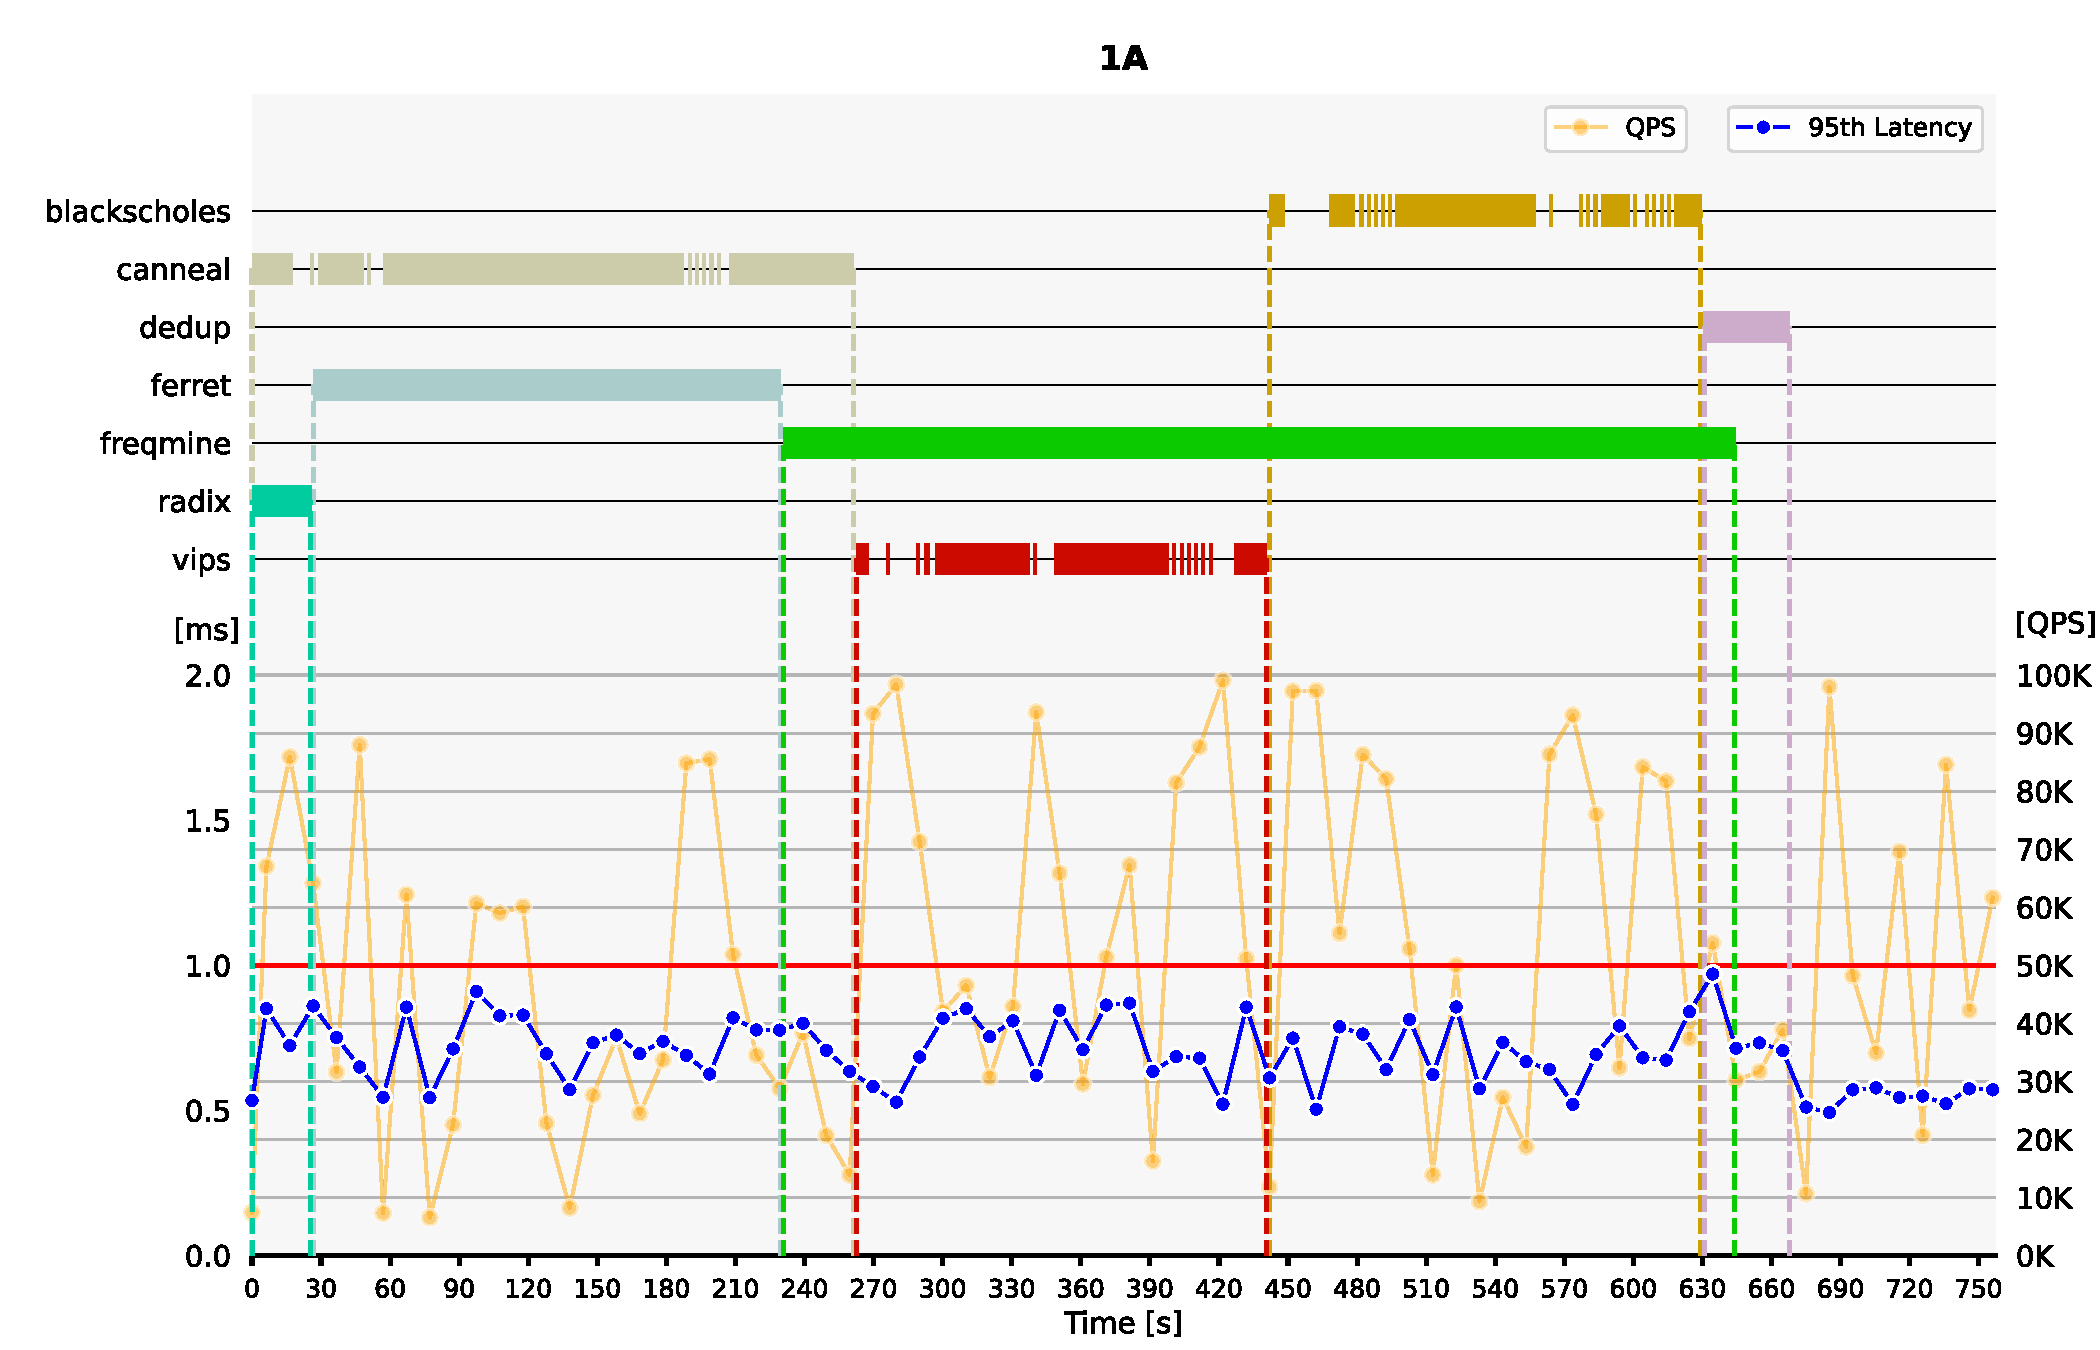
\includegraphics[width=1\linewidth]{figures/part4/plot3_1A.pdf}
        % \caption{Plot 1A}
        \label{fig:plot1A}
    \end{figure}

    \begin{figure}[htbp]
        \centering
        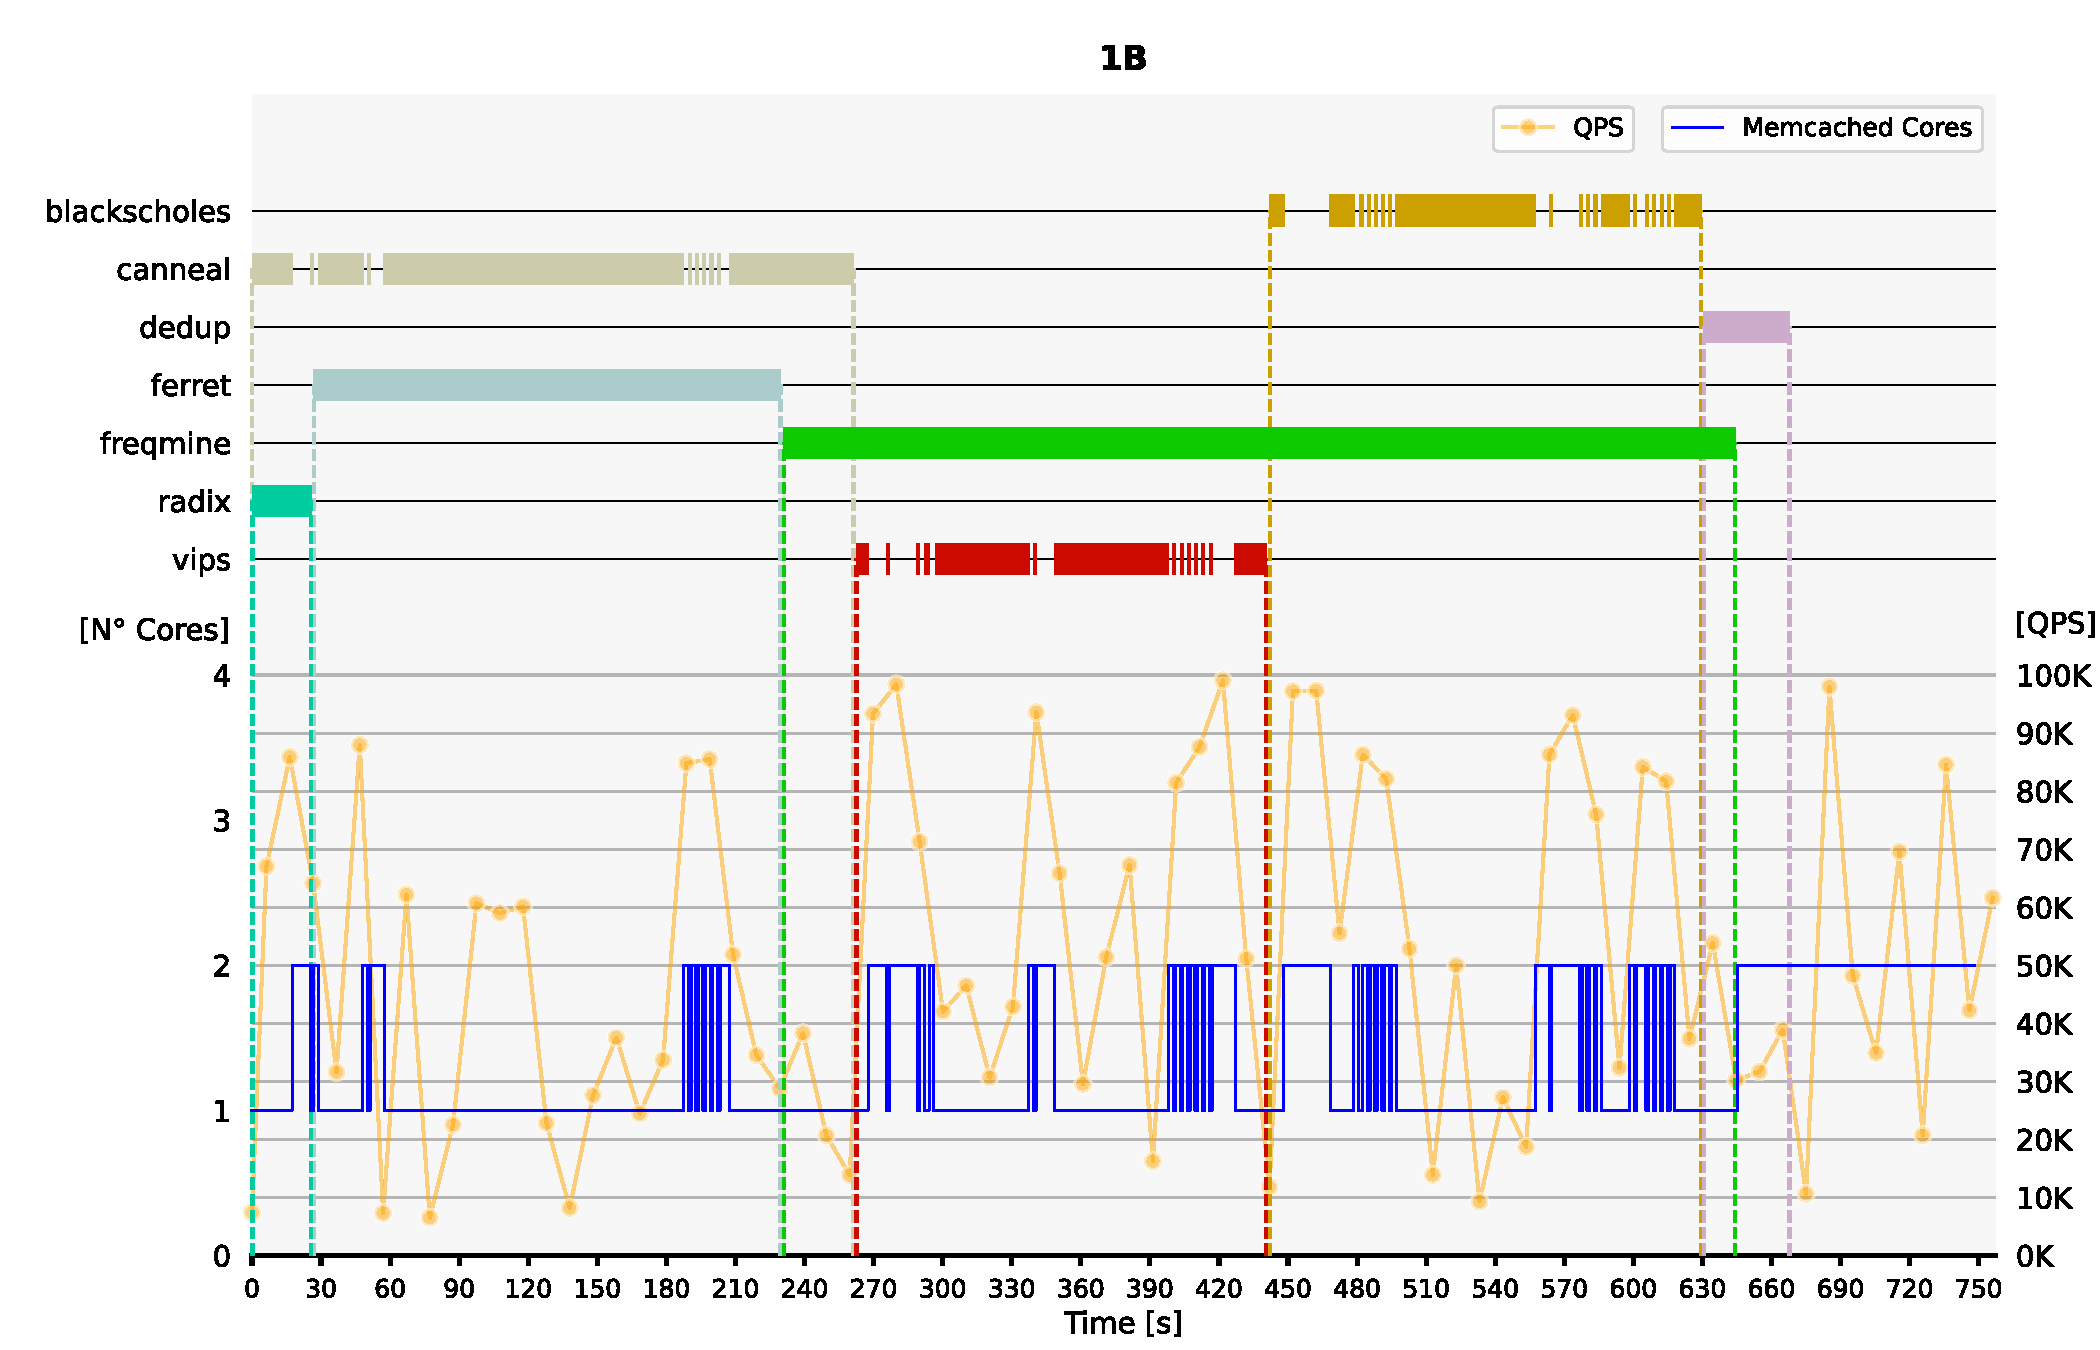
\includegraphics[width=1\linewidth]{figures/part4/plot3_1B.pdf}
        % \caption{Plot 1B}
        \label{fig:plot1B}
    \end{figure}

    \begin{figure}[hhtbpt]
        \centering
        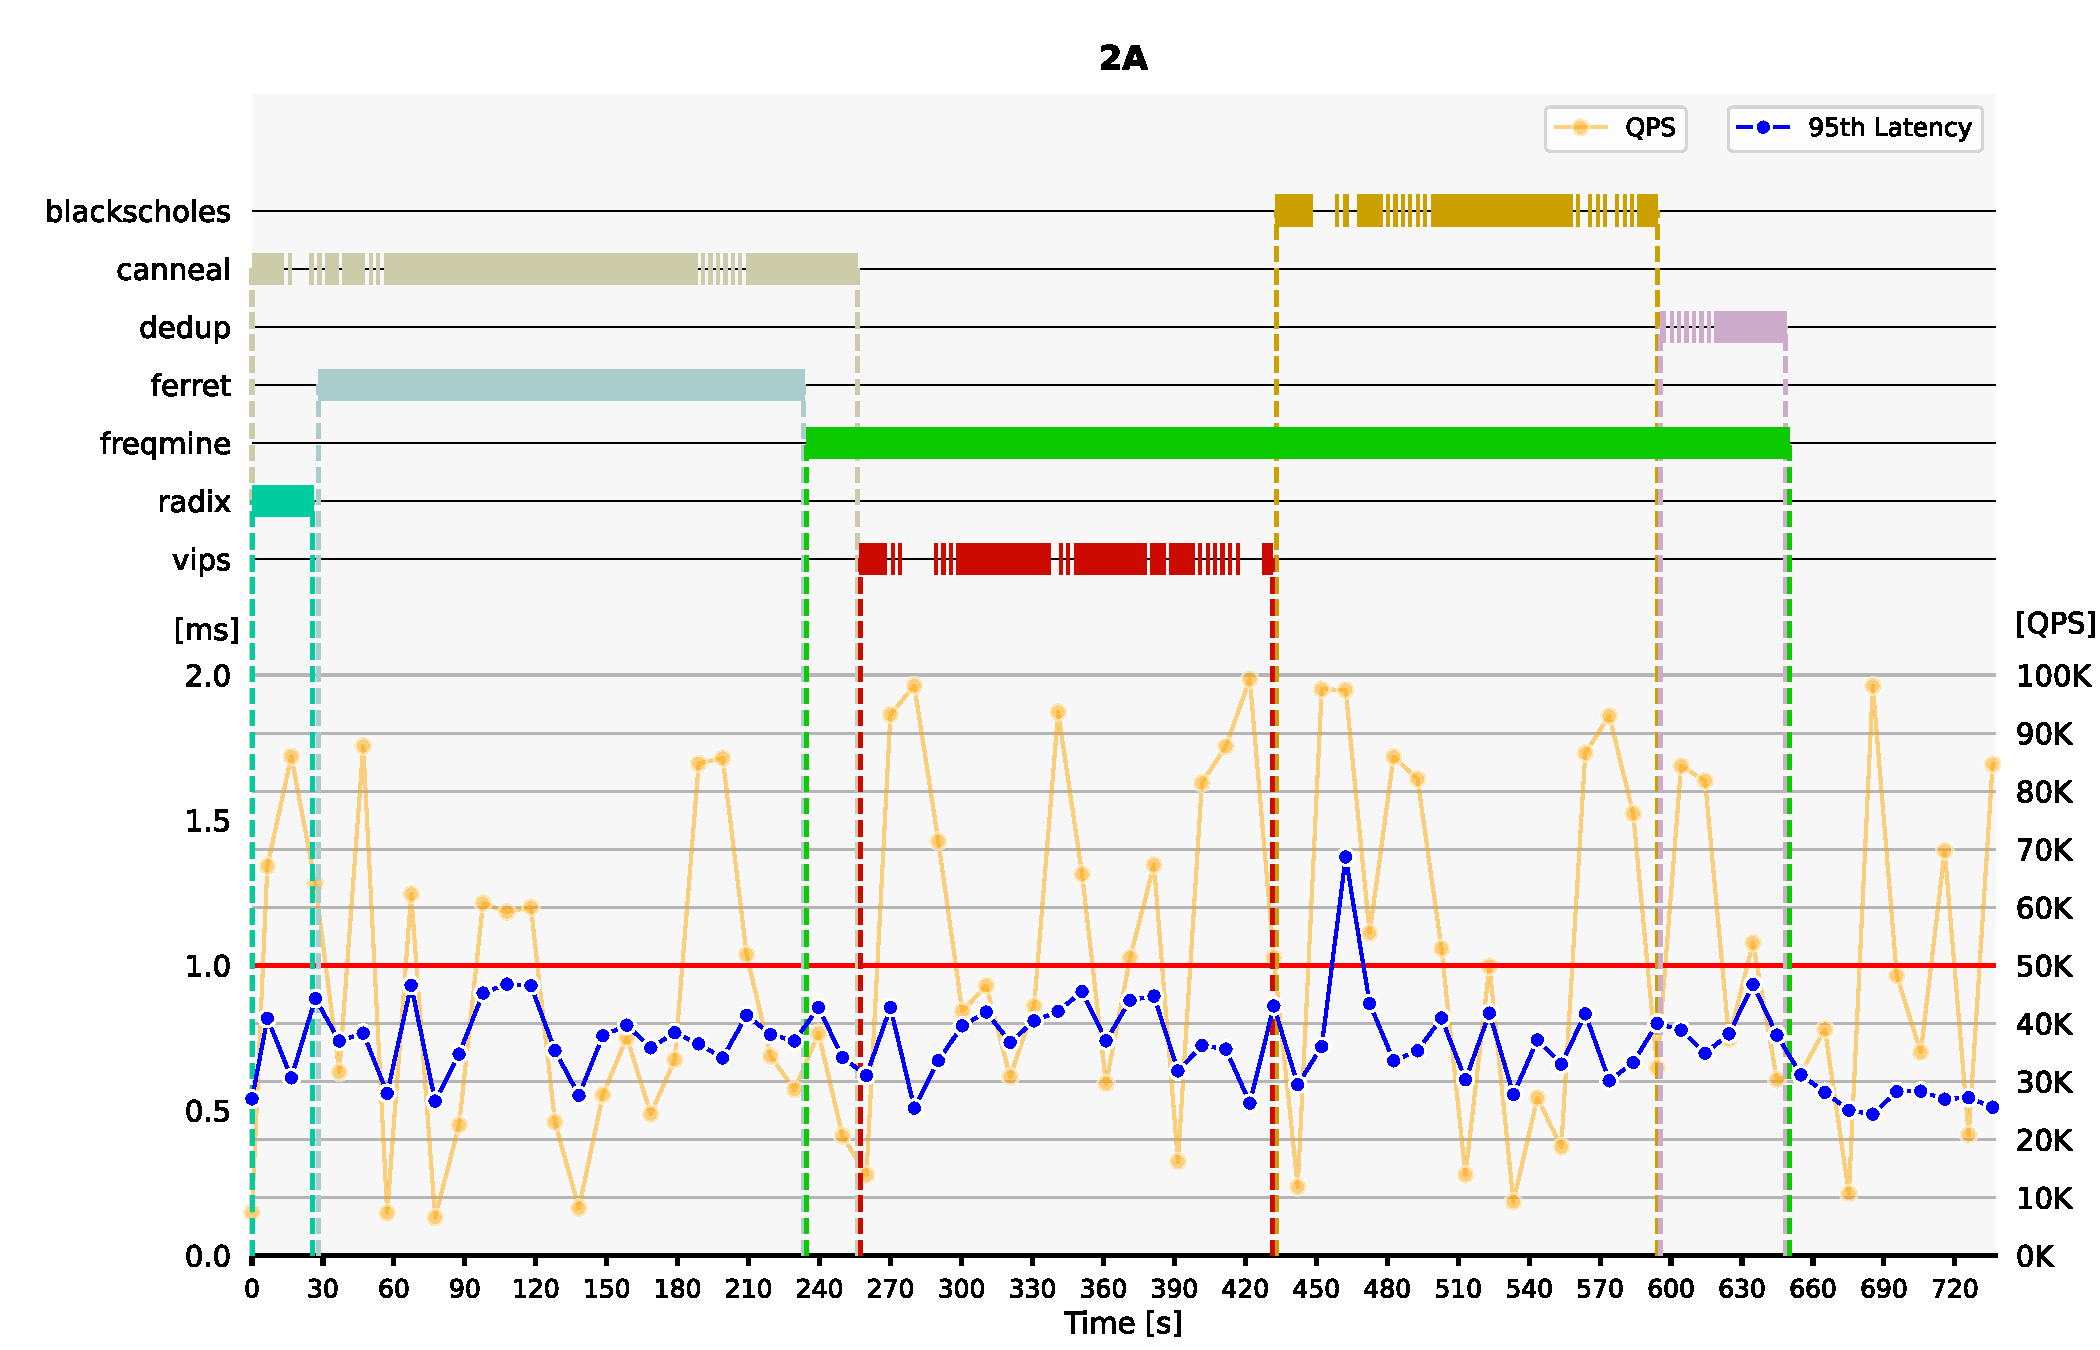
\includegraphics[width=1\linewidth]{figures/part4/plot3_2A.pdf}
        % \caption{Plot 2A}
        \label{fig:plot2A}
    \end{figure}

    \begin{figure}[htbp]
        \centering
        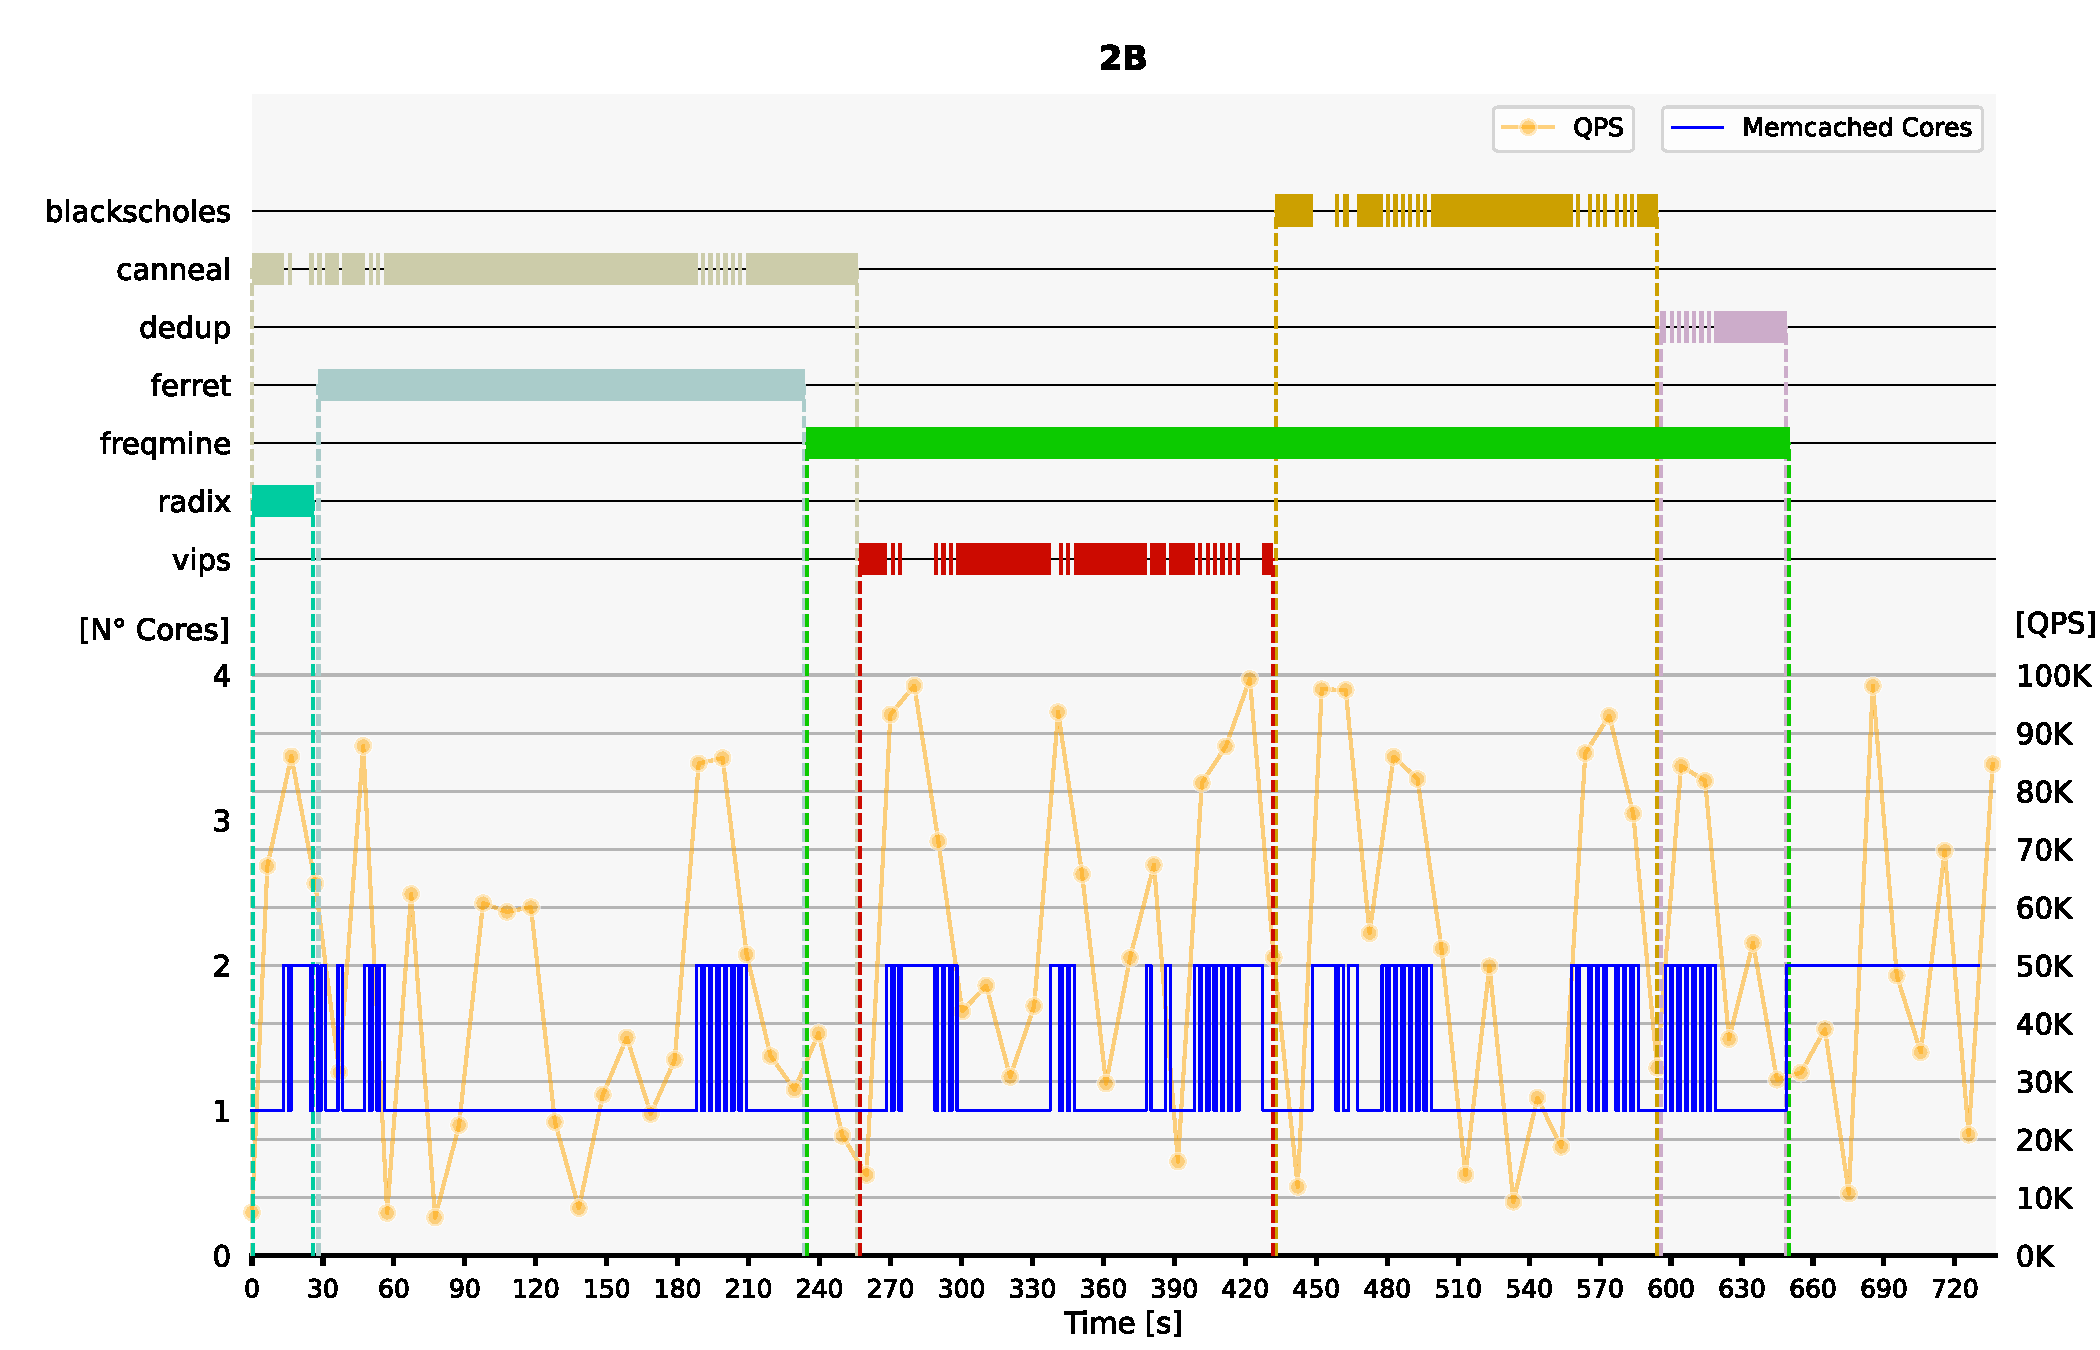
\includegraphics[width=1\linewidth]{figures/part4/plot3_2B.pdf}
        % \caption{Plot 2B}
        \label{fig:plot2B}
    \end{figure}

    \begin{figure}[htbp]
        \centering
        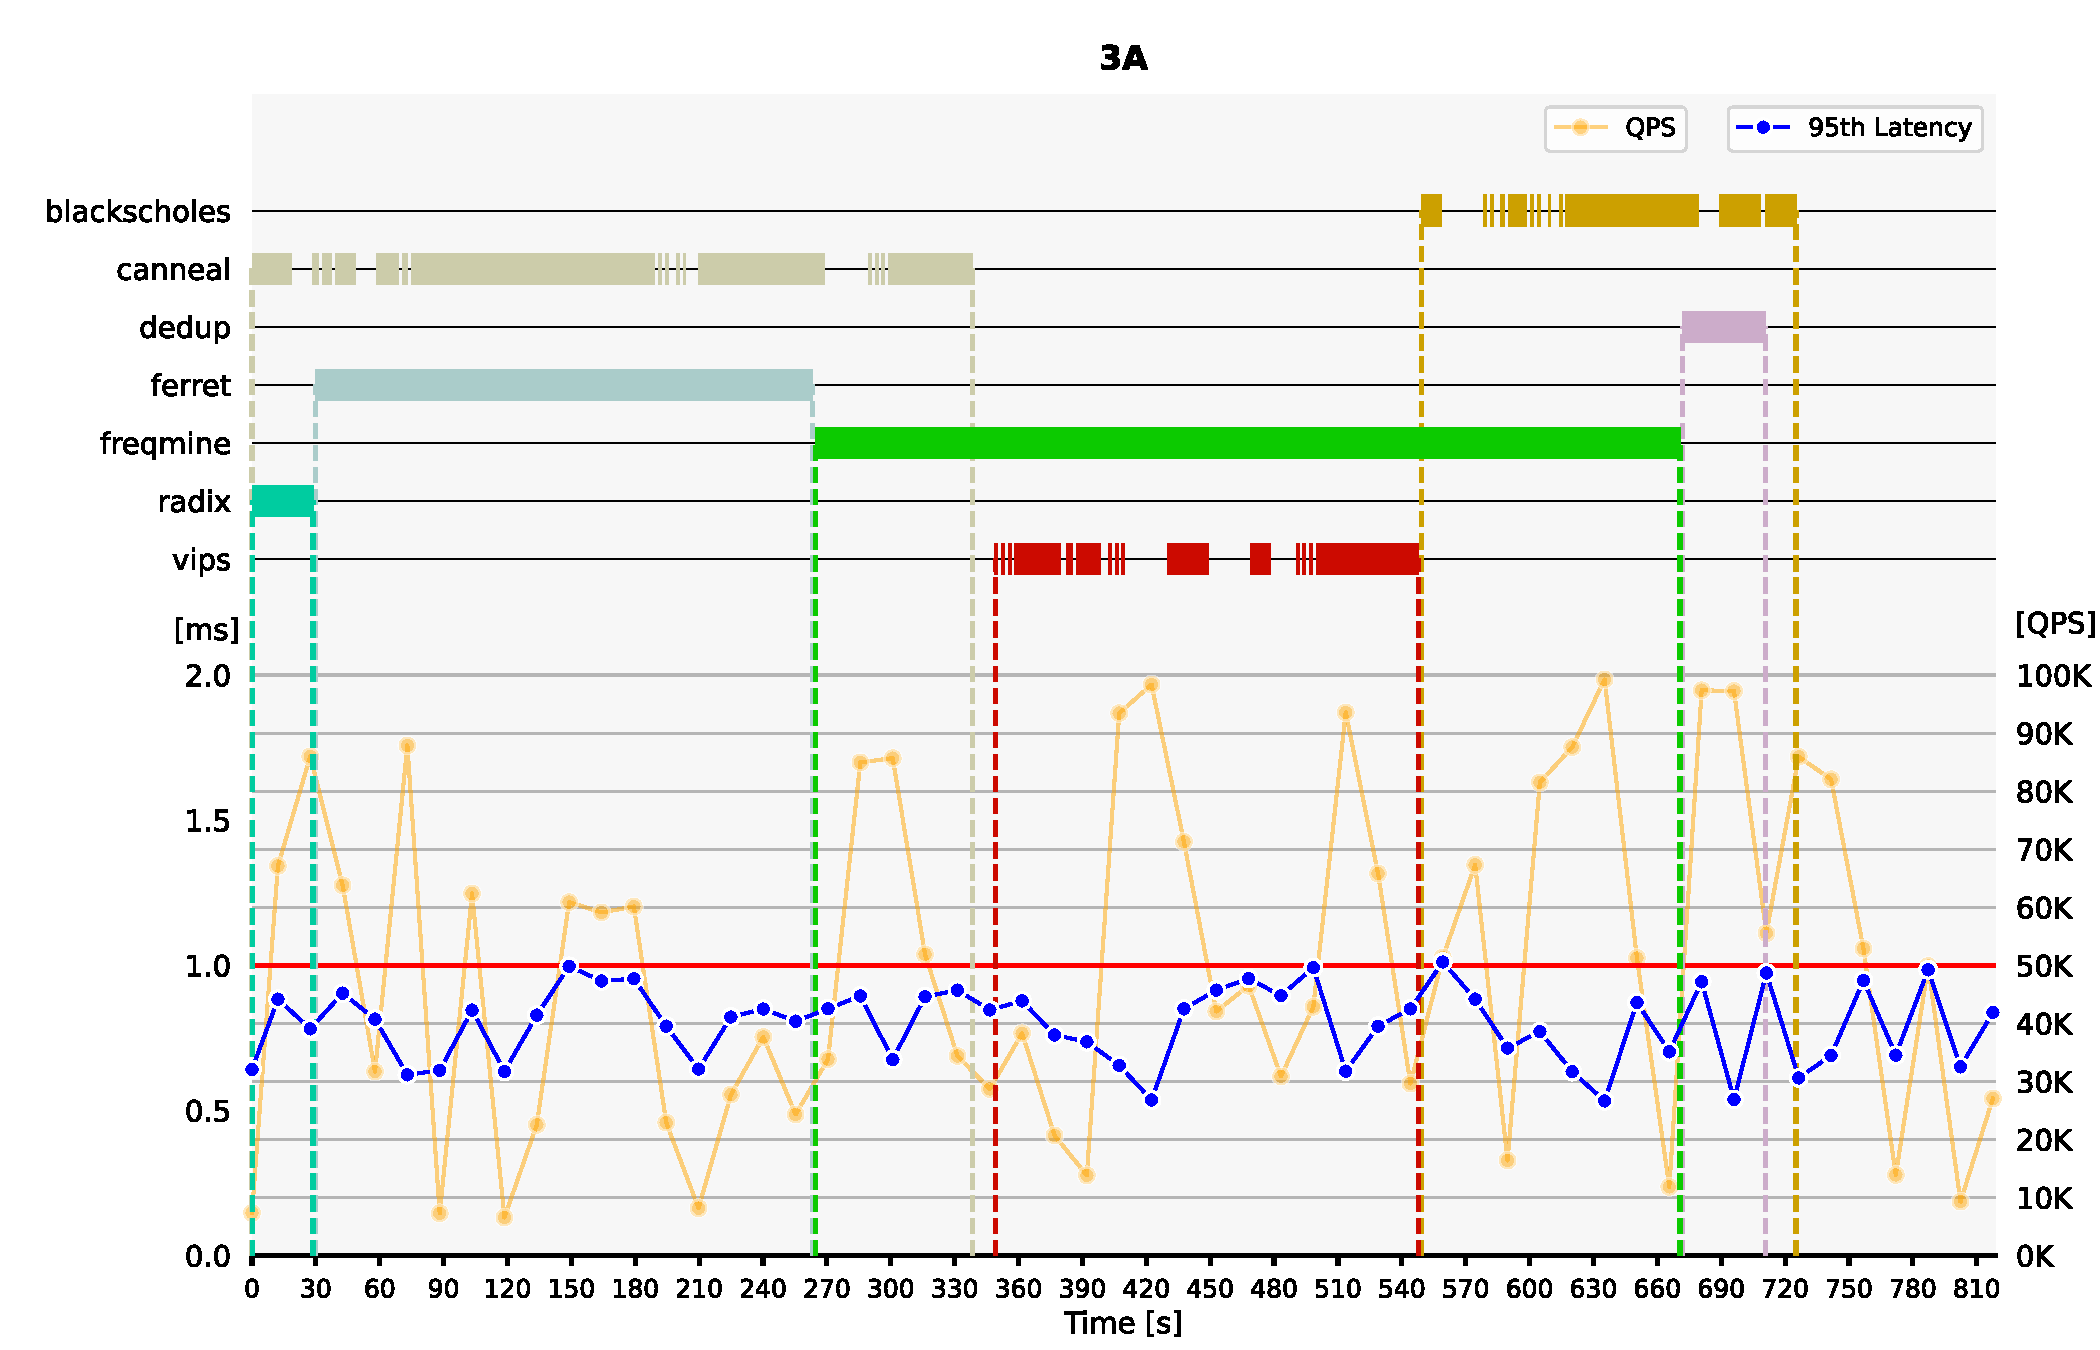
\includegraphics[width=1\linewidth]{figures/part4/plot3_3A.pdf}
        % \caption{Plot 3A}
        \label{fig:plot3A}
    \end{figure}

    \begin{figure}[htbp]
        \centering
        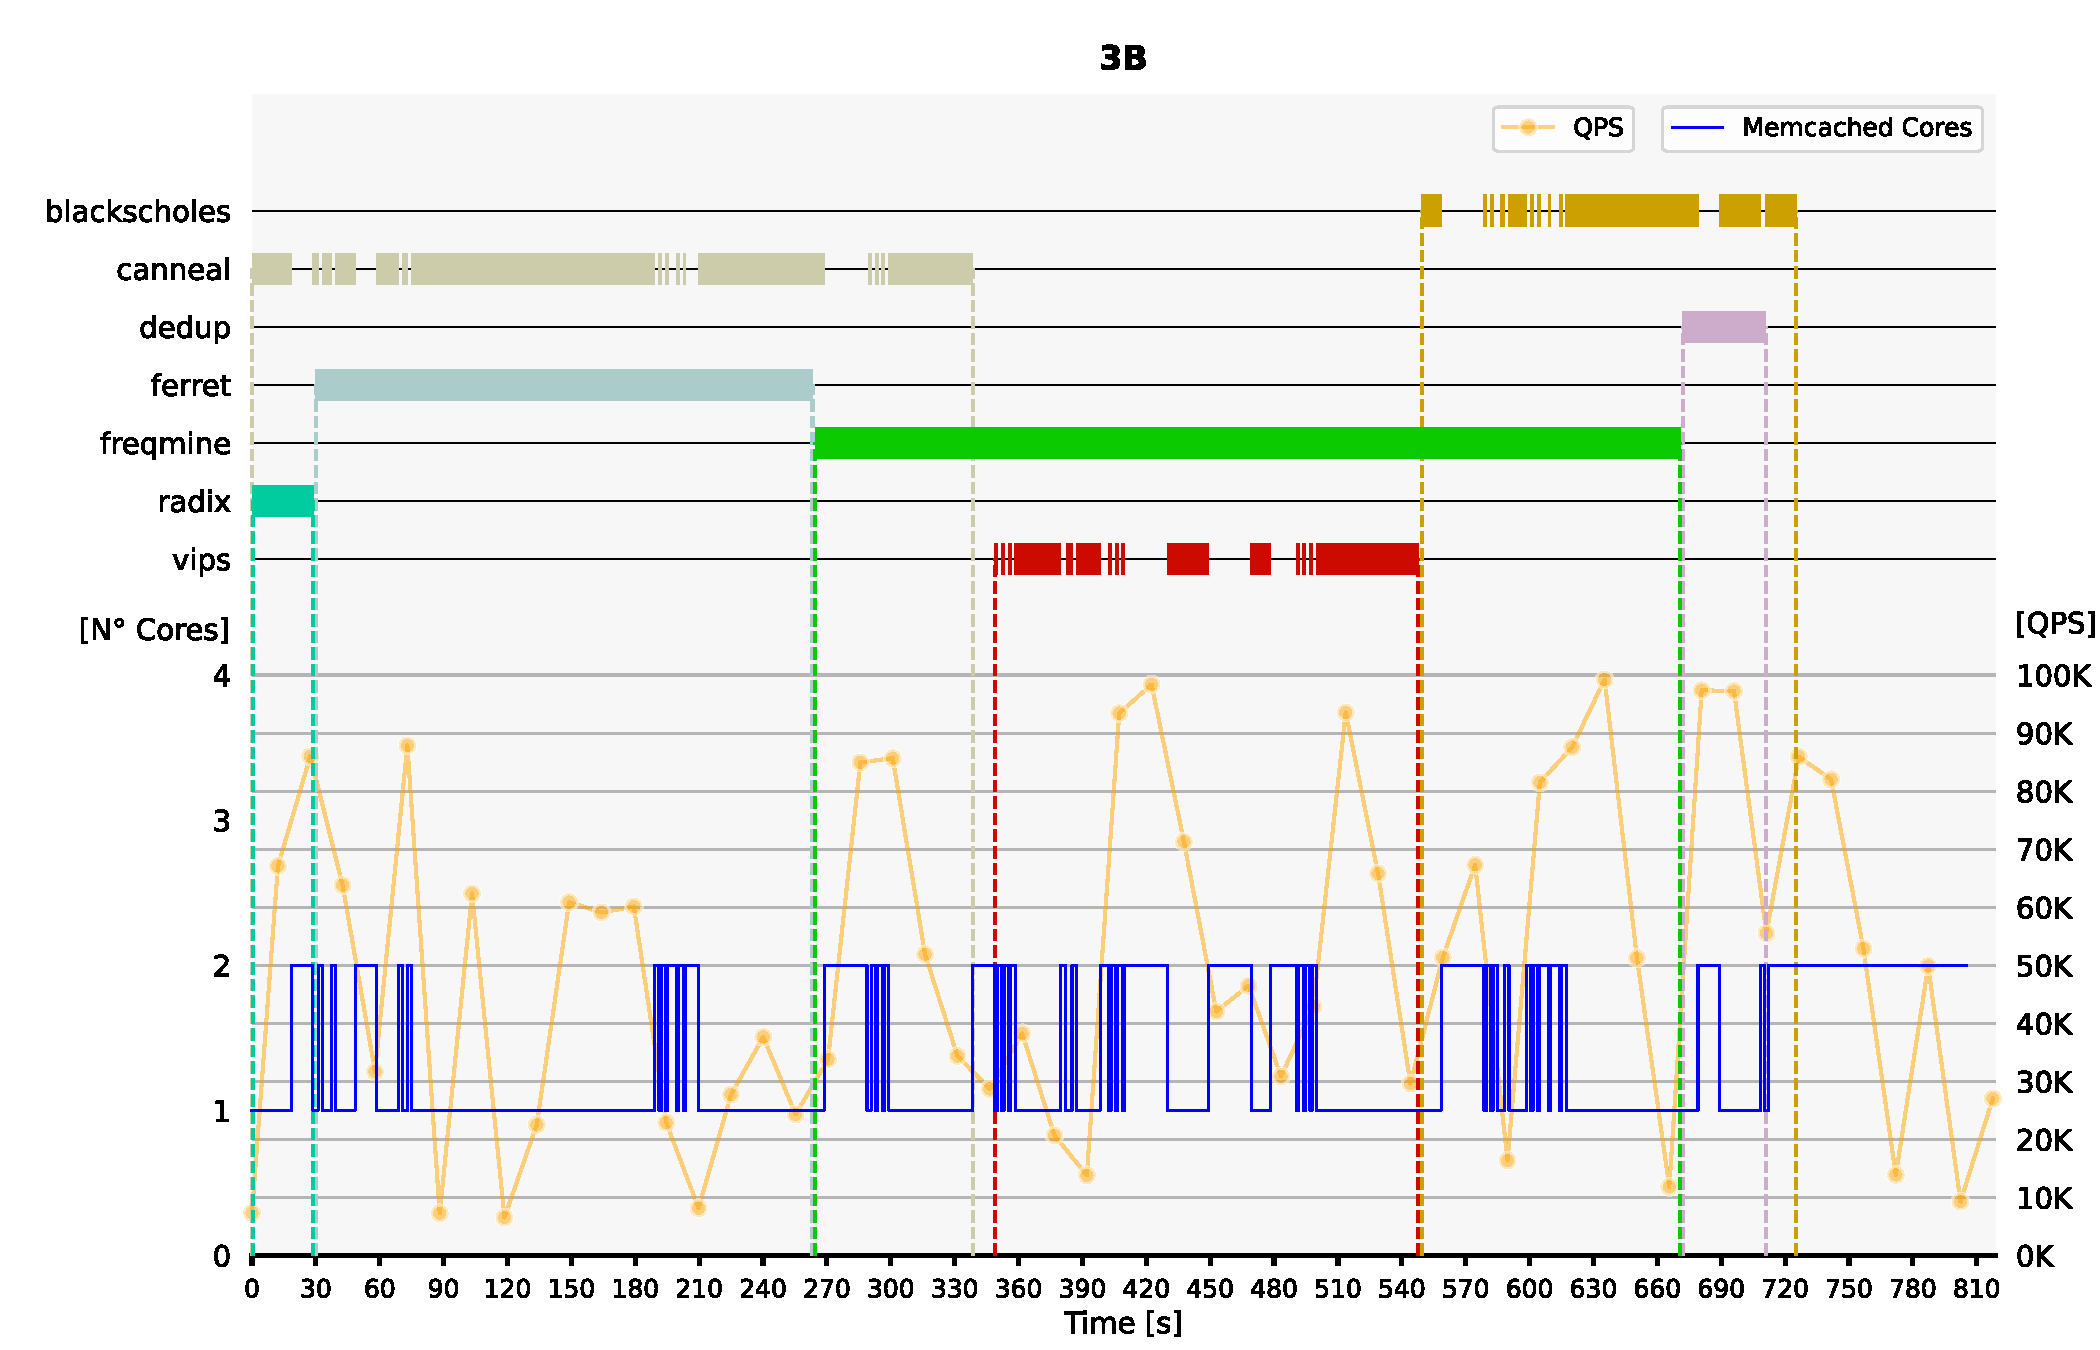
\includegraphics[width=1\linewidth]{figures/part4/plot3_3B.pdf}
        % \caption{Plot 3B}
        \label{fig:plot3B}
    \end{figure}


    \newpage


    \item \textbf{[16 points]} Repeat Part 4 Question 3 with a modified \texttt{mcperf} dynamic load trace with a 5 second time interval (\texttt{qps\_interval}) instead of 10 second time interval. Use the following command: 
    
\begin{Verbatim}[fontsize=\small]
$ ./mcperf -s INTERNAL_MEMCACHED_IP --loadonly 
$ ./mcperf -s INTERNAL_MEMCACHED_IP -a INTERNAL_AGENT_IP \ 
           --noload -T 16 -C 4 -D 4 -Q 1000 -c 4 -t 1800 \ 
           --qps_interval 5 --qps_min 5000 --qps_max 100000 \ 
           --qps_seed 3274
\end{Verbatim}
    
    You do not need to include the plots or table from Question 3 for the 5-second interval. Instead, summarize in 2-3 sentences how your policy performs with the smaller time interval (i.e., higher load variability) compared to the original load trace in Question 3. 

    \textbf{Summary:} Managing the 5-second interval trace was more challenging than the 10-second one, reflected by higher Service Level Objective (SLO) violation ratios. The first and second experiments recorded SLO violation ratios around 3.5\% (5/134), whereas before we had rarely any. The total runtime didn't actually change compared with the 10-second interval trace.

    What is the SLO violation ratio for memcached (i.e., the number of datapoints with 95th percentile latency $>$ 1ms, as a fraction of the total number of datapoints) with the 5-second time interval trace? 
    
    \textbf{Answer:} The SLO violation ratio for memcached with the 5-second time interval trace is approximately 3.73\% (5/134) for the first experiment and 2.98\% (4/134) with the 5-second time interval trace. Therefore, we were not consistently under 3\%.
    
    What is the smallest \texttt{qps\_interval} you can use in the load trace that allows your controller to respond fast enough to keep the memcached SLO violation ratio under 3\%? 
    
    \textbf{Answer:} The smallest interval was 6. We did three different runs, all with SLOs under 3\% with the following \texttt{qps\_interval} values: 2/134 = 1.49\%, 4/134 = 2.98\%, 2/134 = 1.49\%.

    What is the reasoning behind this specific value? Explain which features of your controller affect the smallest \texttt{qps\_interval} interval you proposed.
  
    \textbf{Answer:} The features of the controller that may not be able to respond to faster QPS include the CPU utilization monitoring, the container management, and the dynamic container adjustment strategy as well the taskset command of memcached.

    If the QPS changes too frequently, the controller may not be able to keep up with the changes and respond quickly enough to prevent SLO violations. For example, if there is a sudden drop in CPU utilization between two peaks, we may respond to the drop and downscale memcached. However, if the next peak comes, we may not hbe able to handle the peak and upscale again memcached without violating the SLO. However, if we are not very responsive the time to execute PARSEC jobs will increase, so there should be a balance between responsiveness and stability.
    
    \vspace{4cm}

    Use this \texttt{qps\_interval} in the command above and collect results for three runs. Include the same types of plots (1A, 1B, 2A, 2B, 3A, 3B) and table as in Question 3. 
    
    \textbf{Plots:} % Put your plots here
    
    \begin{table}[ht]
        \centering
        \begin{tabular}{ |c|c|c|c|c|} 
            \hline
            job name & mean time [s] & std [s] \\ \hline \hline
            \coloredcell{blackscholes}     & 111.75 & 2.40 \\  \hline
            \coloredcell{canneal}          & 225.92 & 0.45\\  \hline
            \coloredcell{dedup}            & 38.18  & 2.86 \\  \hline
            \coloredcell{ferret}           & 202.06 & 0.57 \\  \hline
            \coloredcell{freqmine}         & 411.90 & 4.81 \\  \hline
            \coloredcell{radix}            & 25.16 & 0.36\\  \hline
            \coloredcell{vips}             & 116.26 & 1.22 \\  \hline
            total time      & 665.29 & 11.33\\  \hline
        \end{tabular}
    \end{table}

    \vspace{10cm}

    \begin{figure}[htbp]
        \centering
        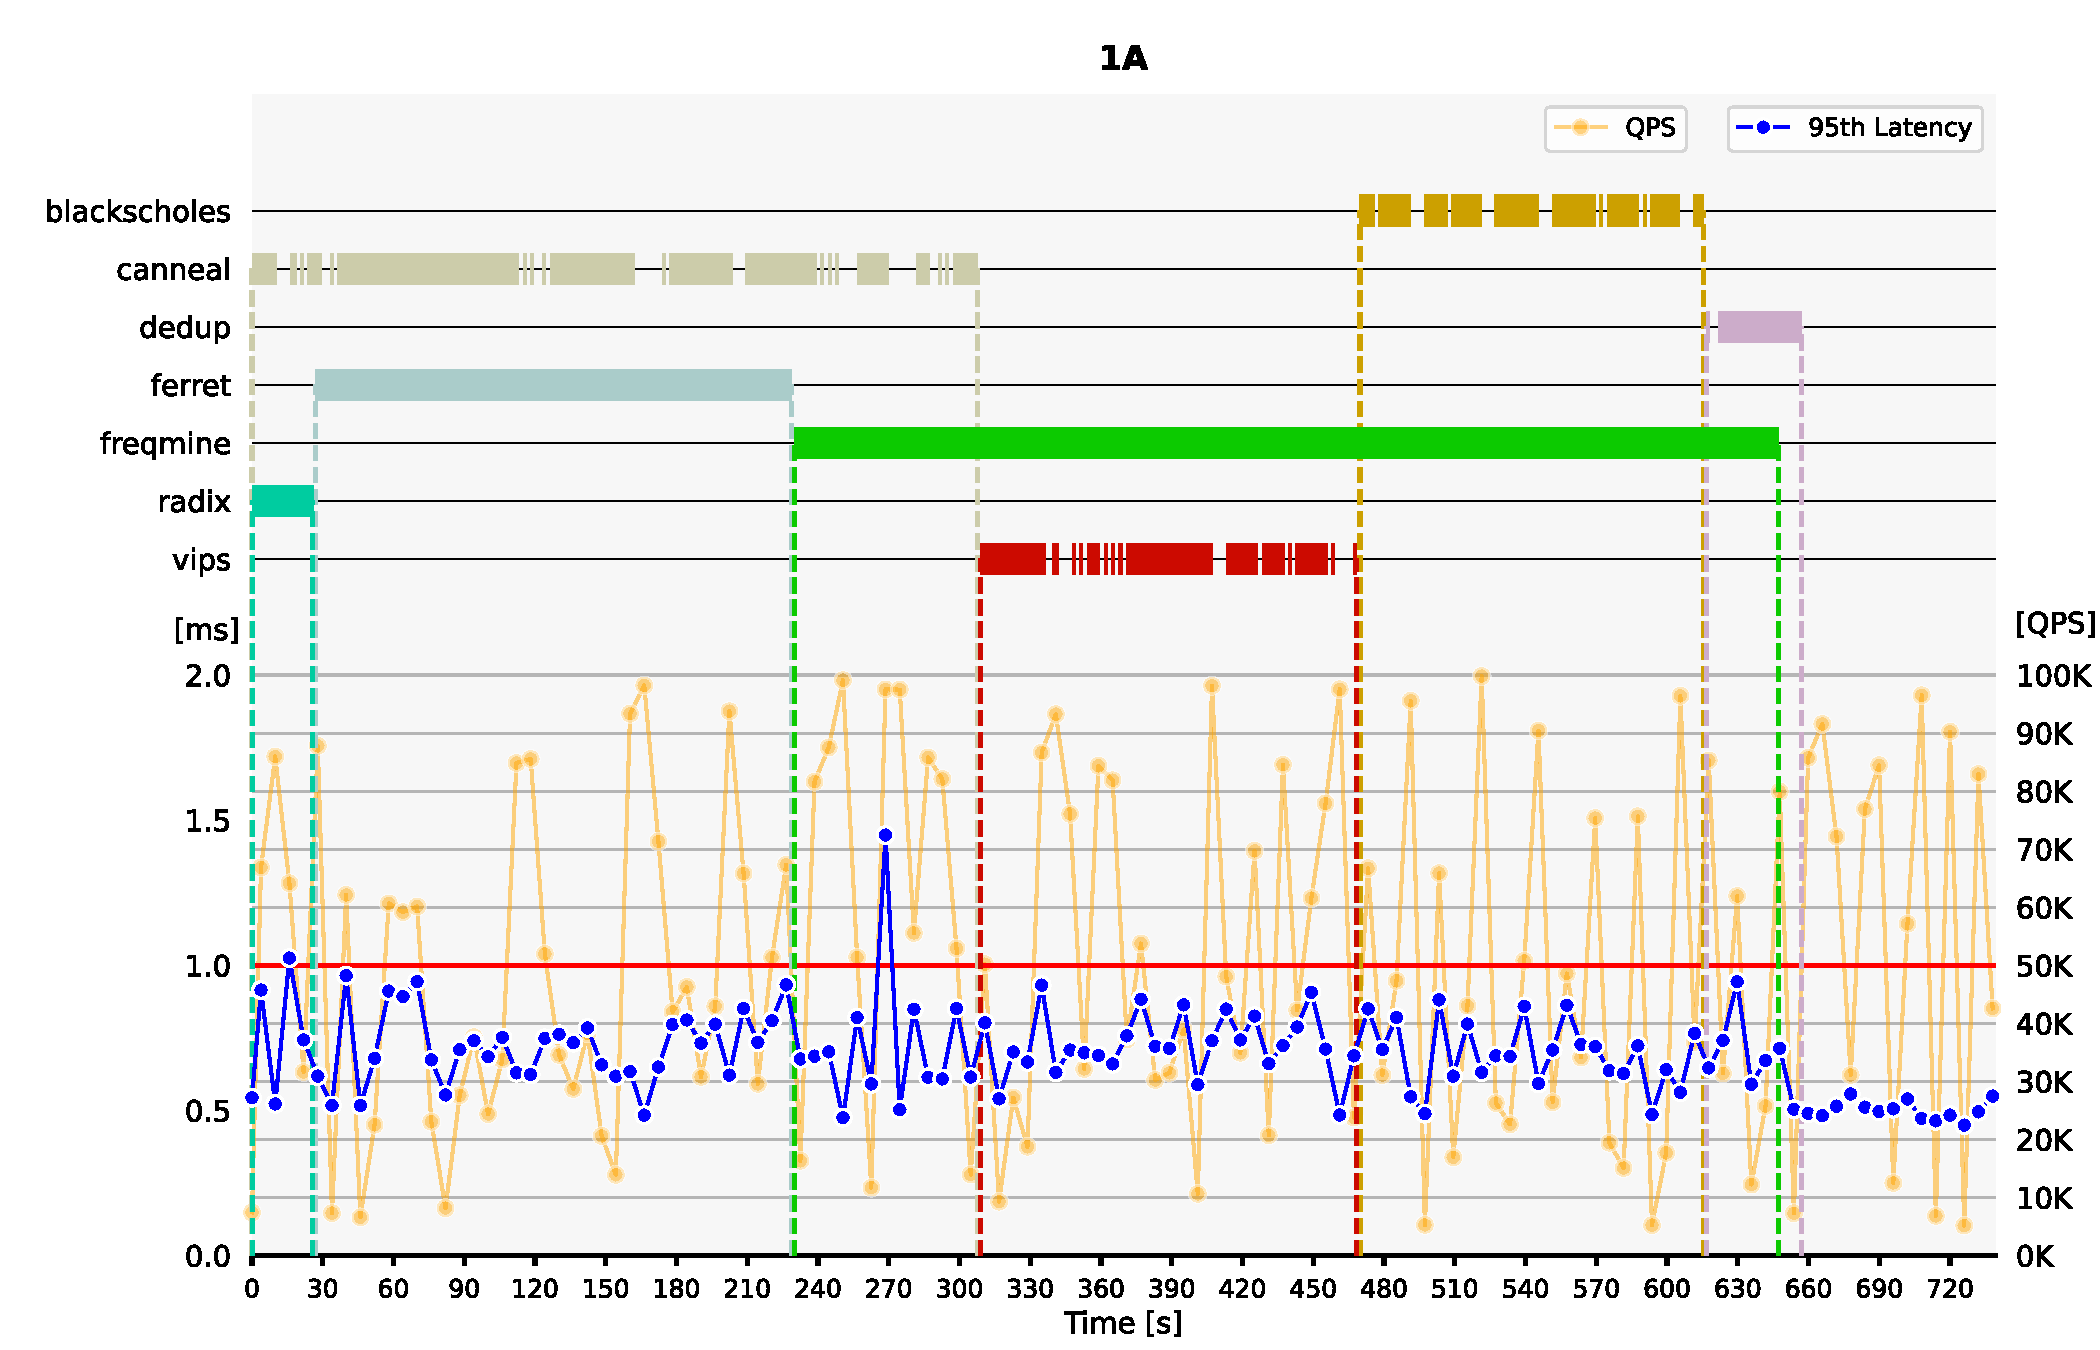
\includegraphics[width=1\linewidth]{figures/part4/plot4_1A.pdf}
        % \caption{Plot 1A}
        \label{fig:plot1A-2}
    \end{figure}

    \begin{figure}[htbp]
        \centering
        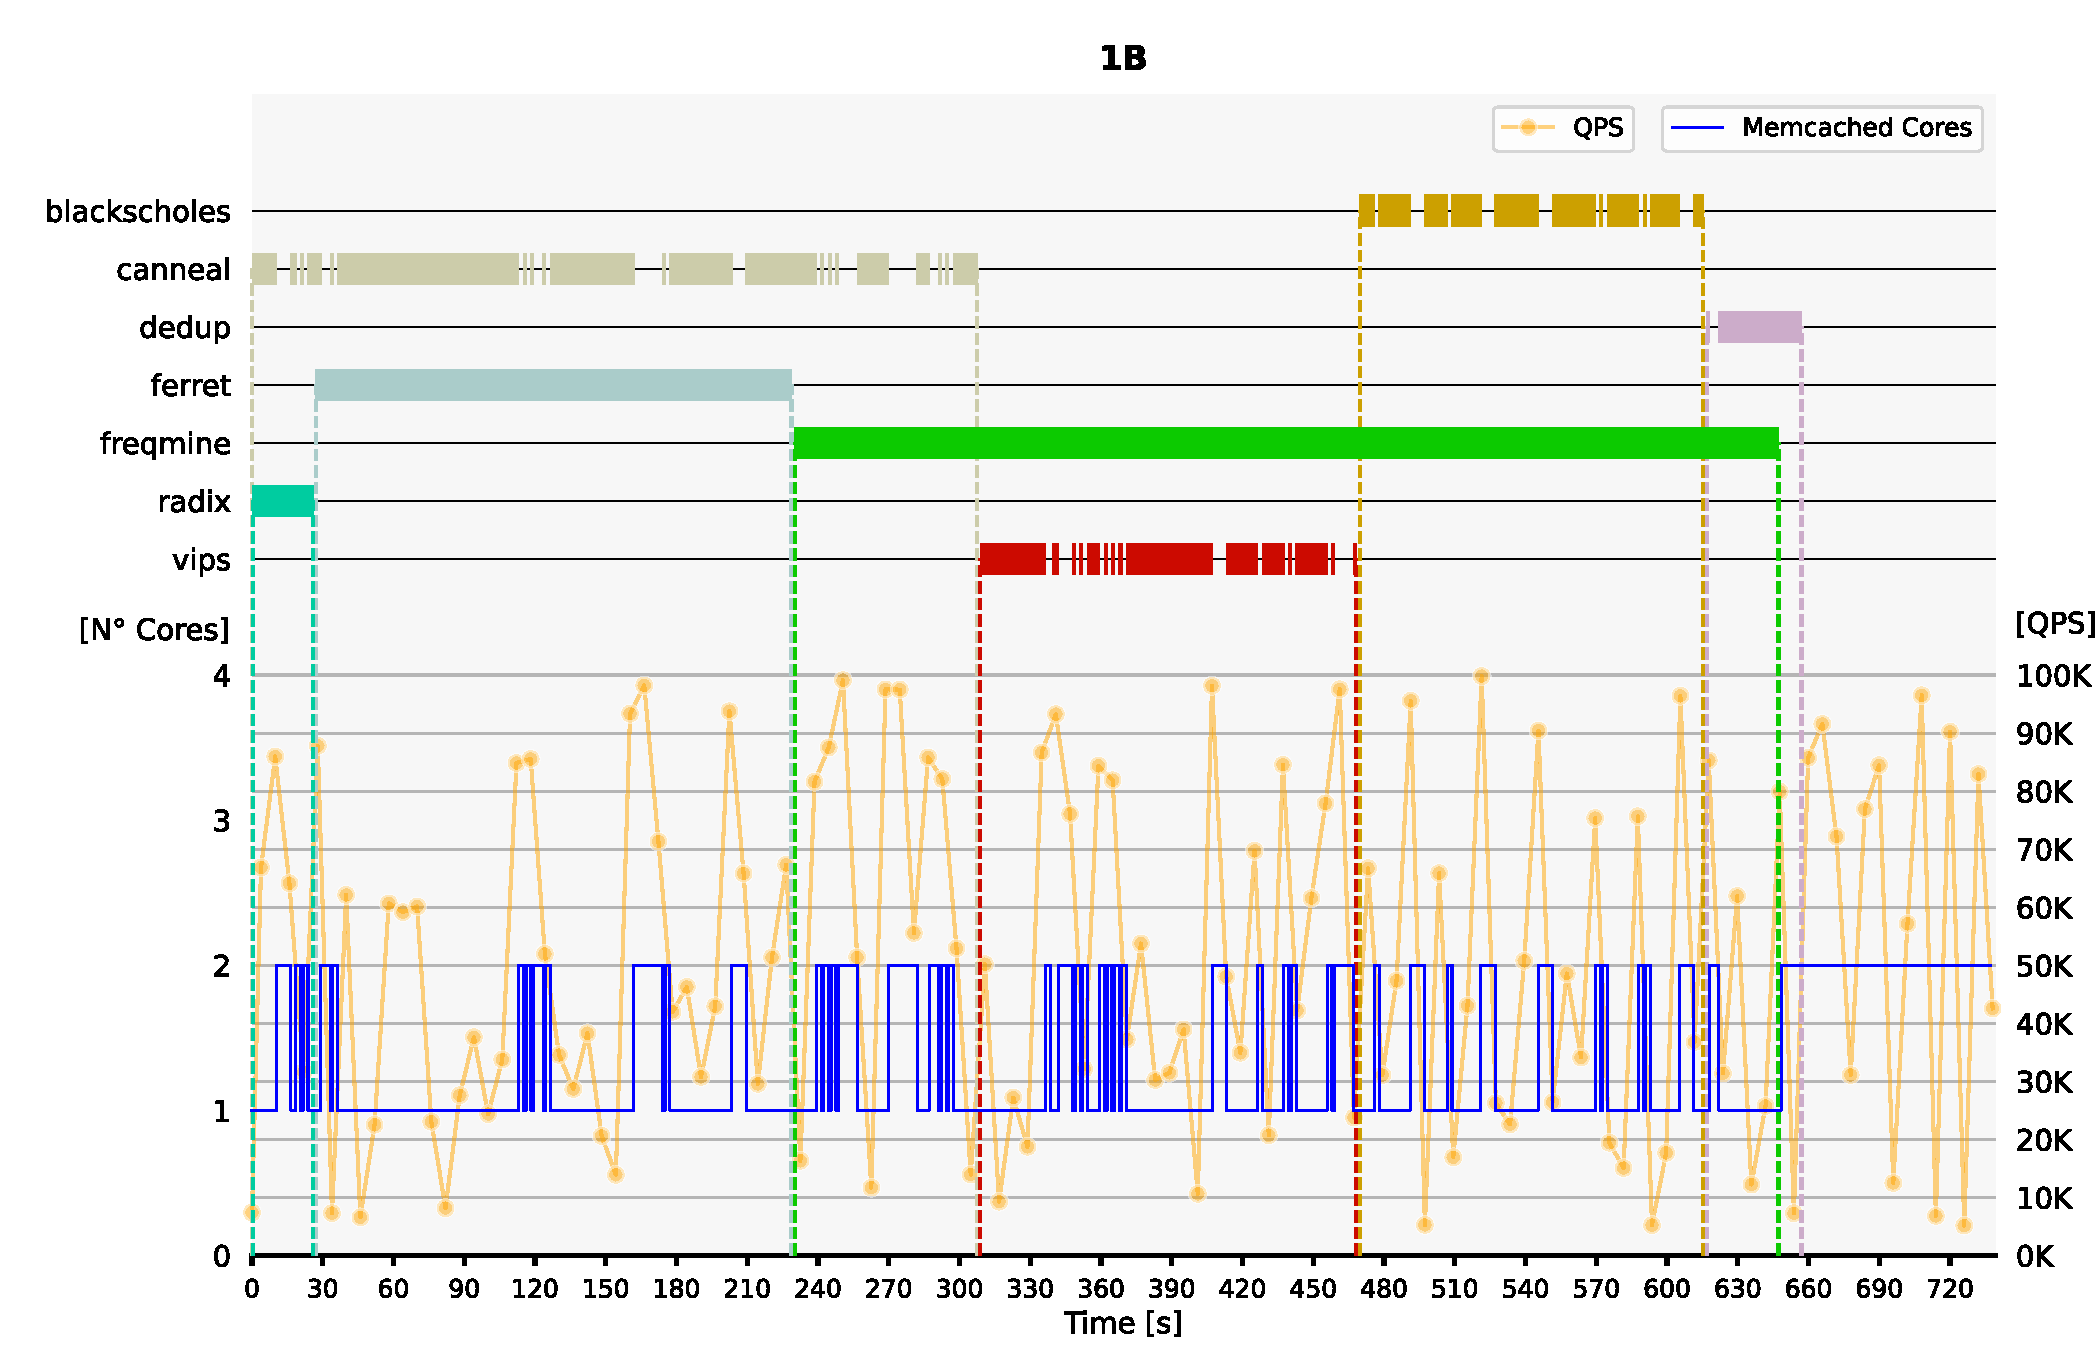
\includegraphics[width=1\linewidth]{figures/part4/plot4_1B.pdf}
        % \caption{Plot 1B}
        \label{fig:plot1B-2}
    \end{figure}

    \begin{figure}[htbp]
        \centering
        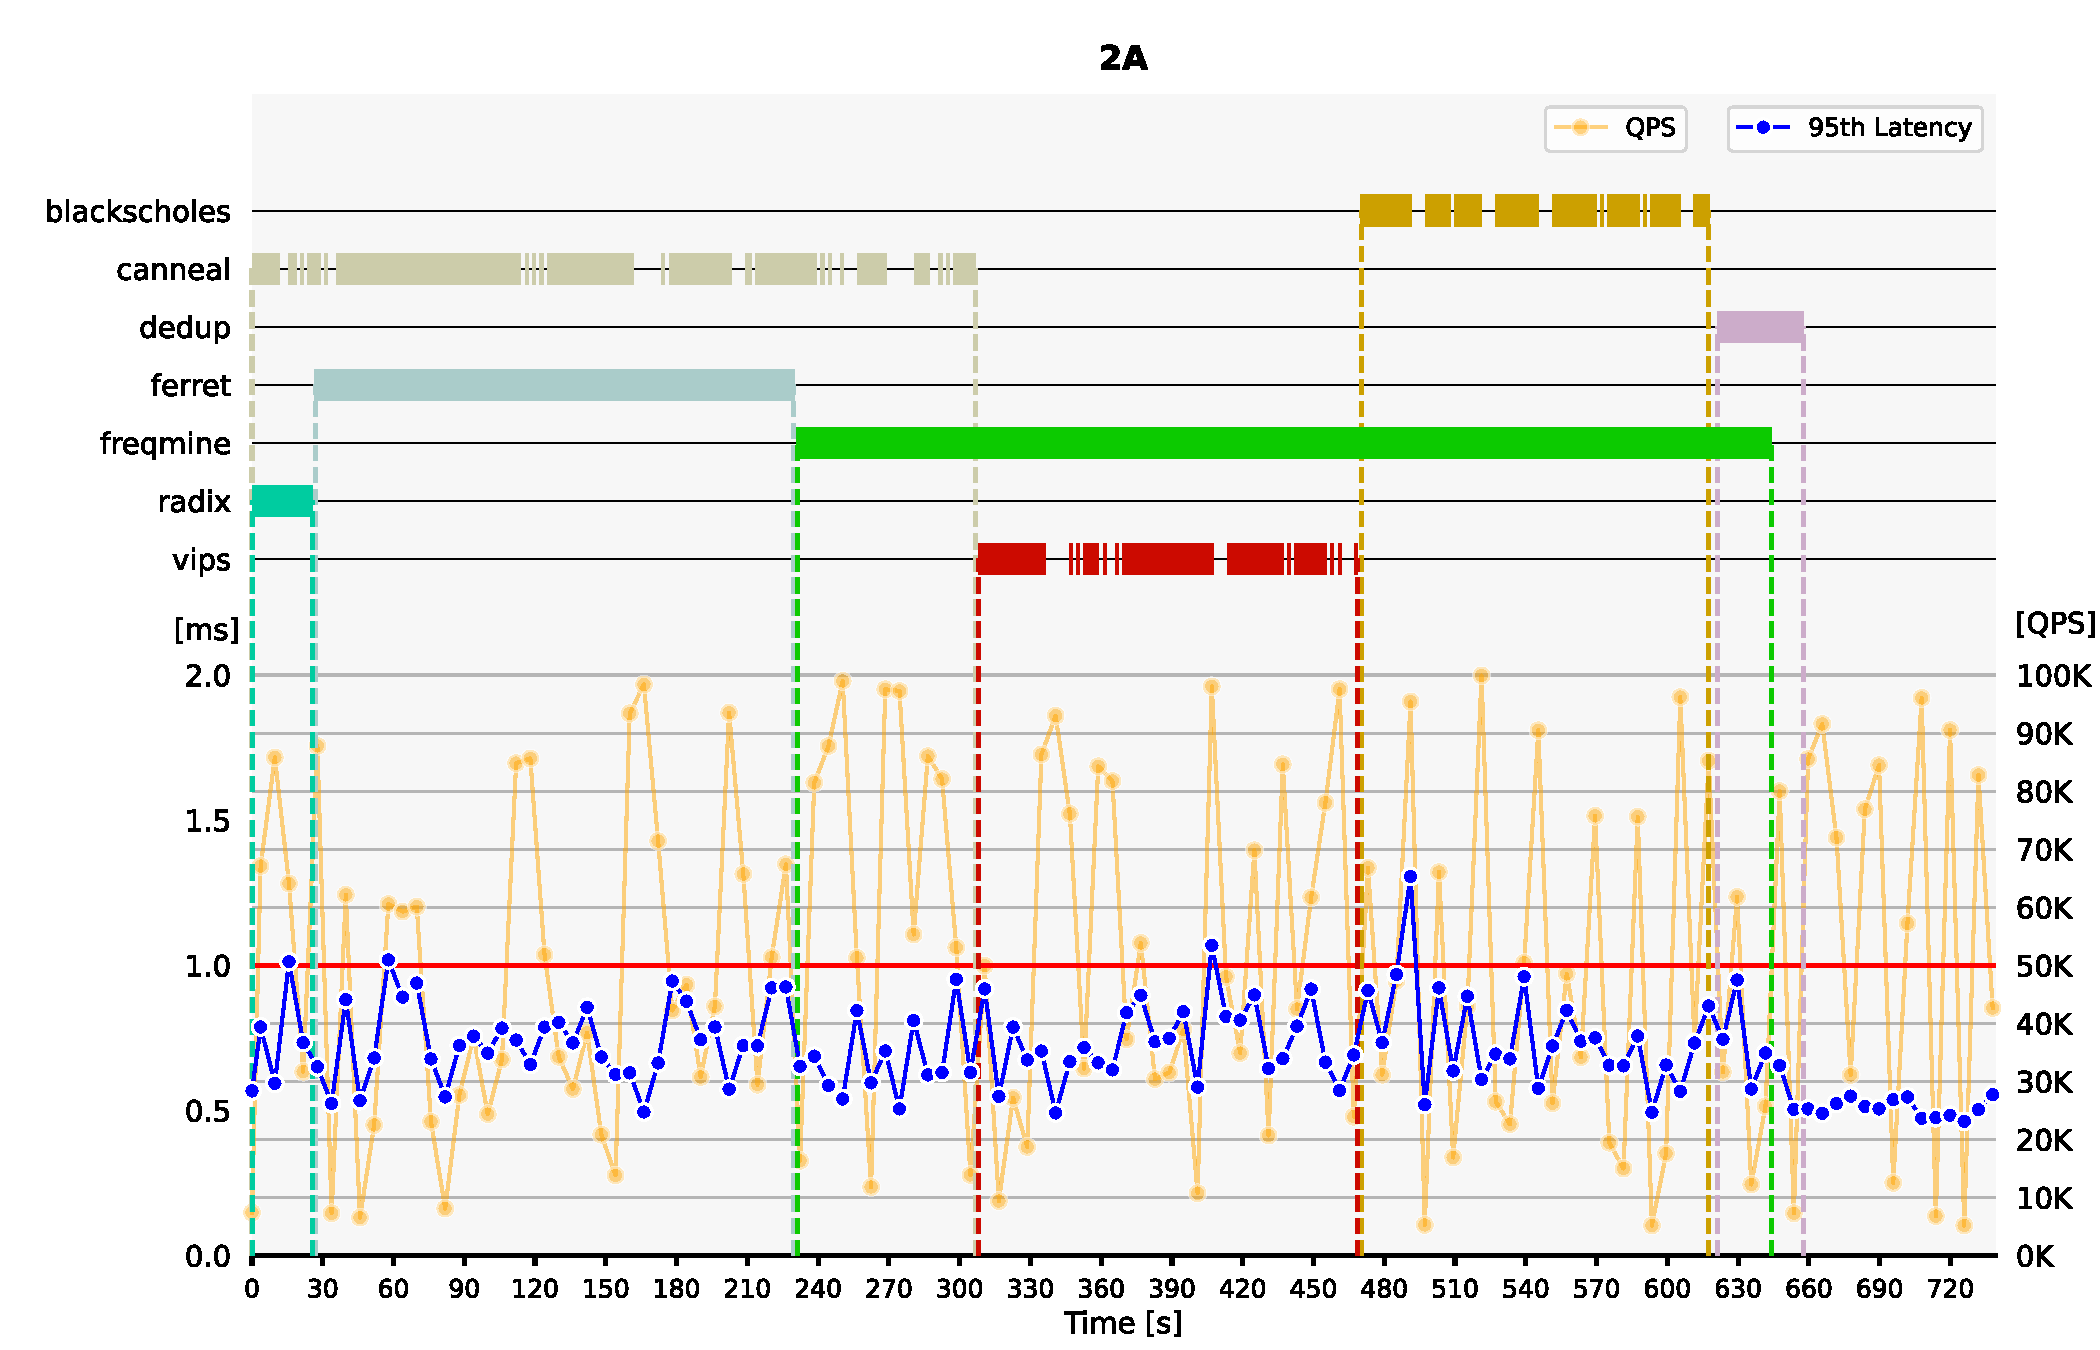
\includegraphics[width=1\linewidth]{figures/part4/plot4_2A.pdf}
        % \caption{Plot 2A}
        \label{fig:plot2A-2}
    \end{figure}

    \begin{figure}[htbp]
        \centering
        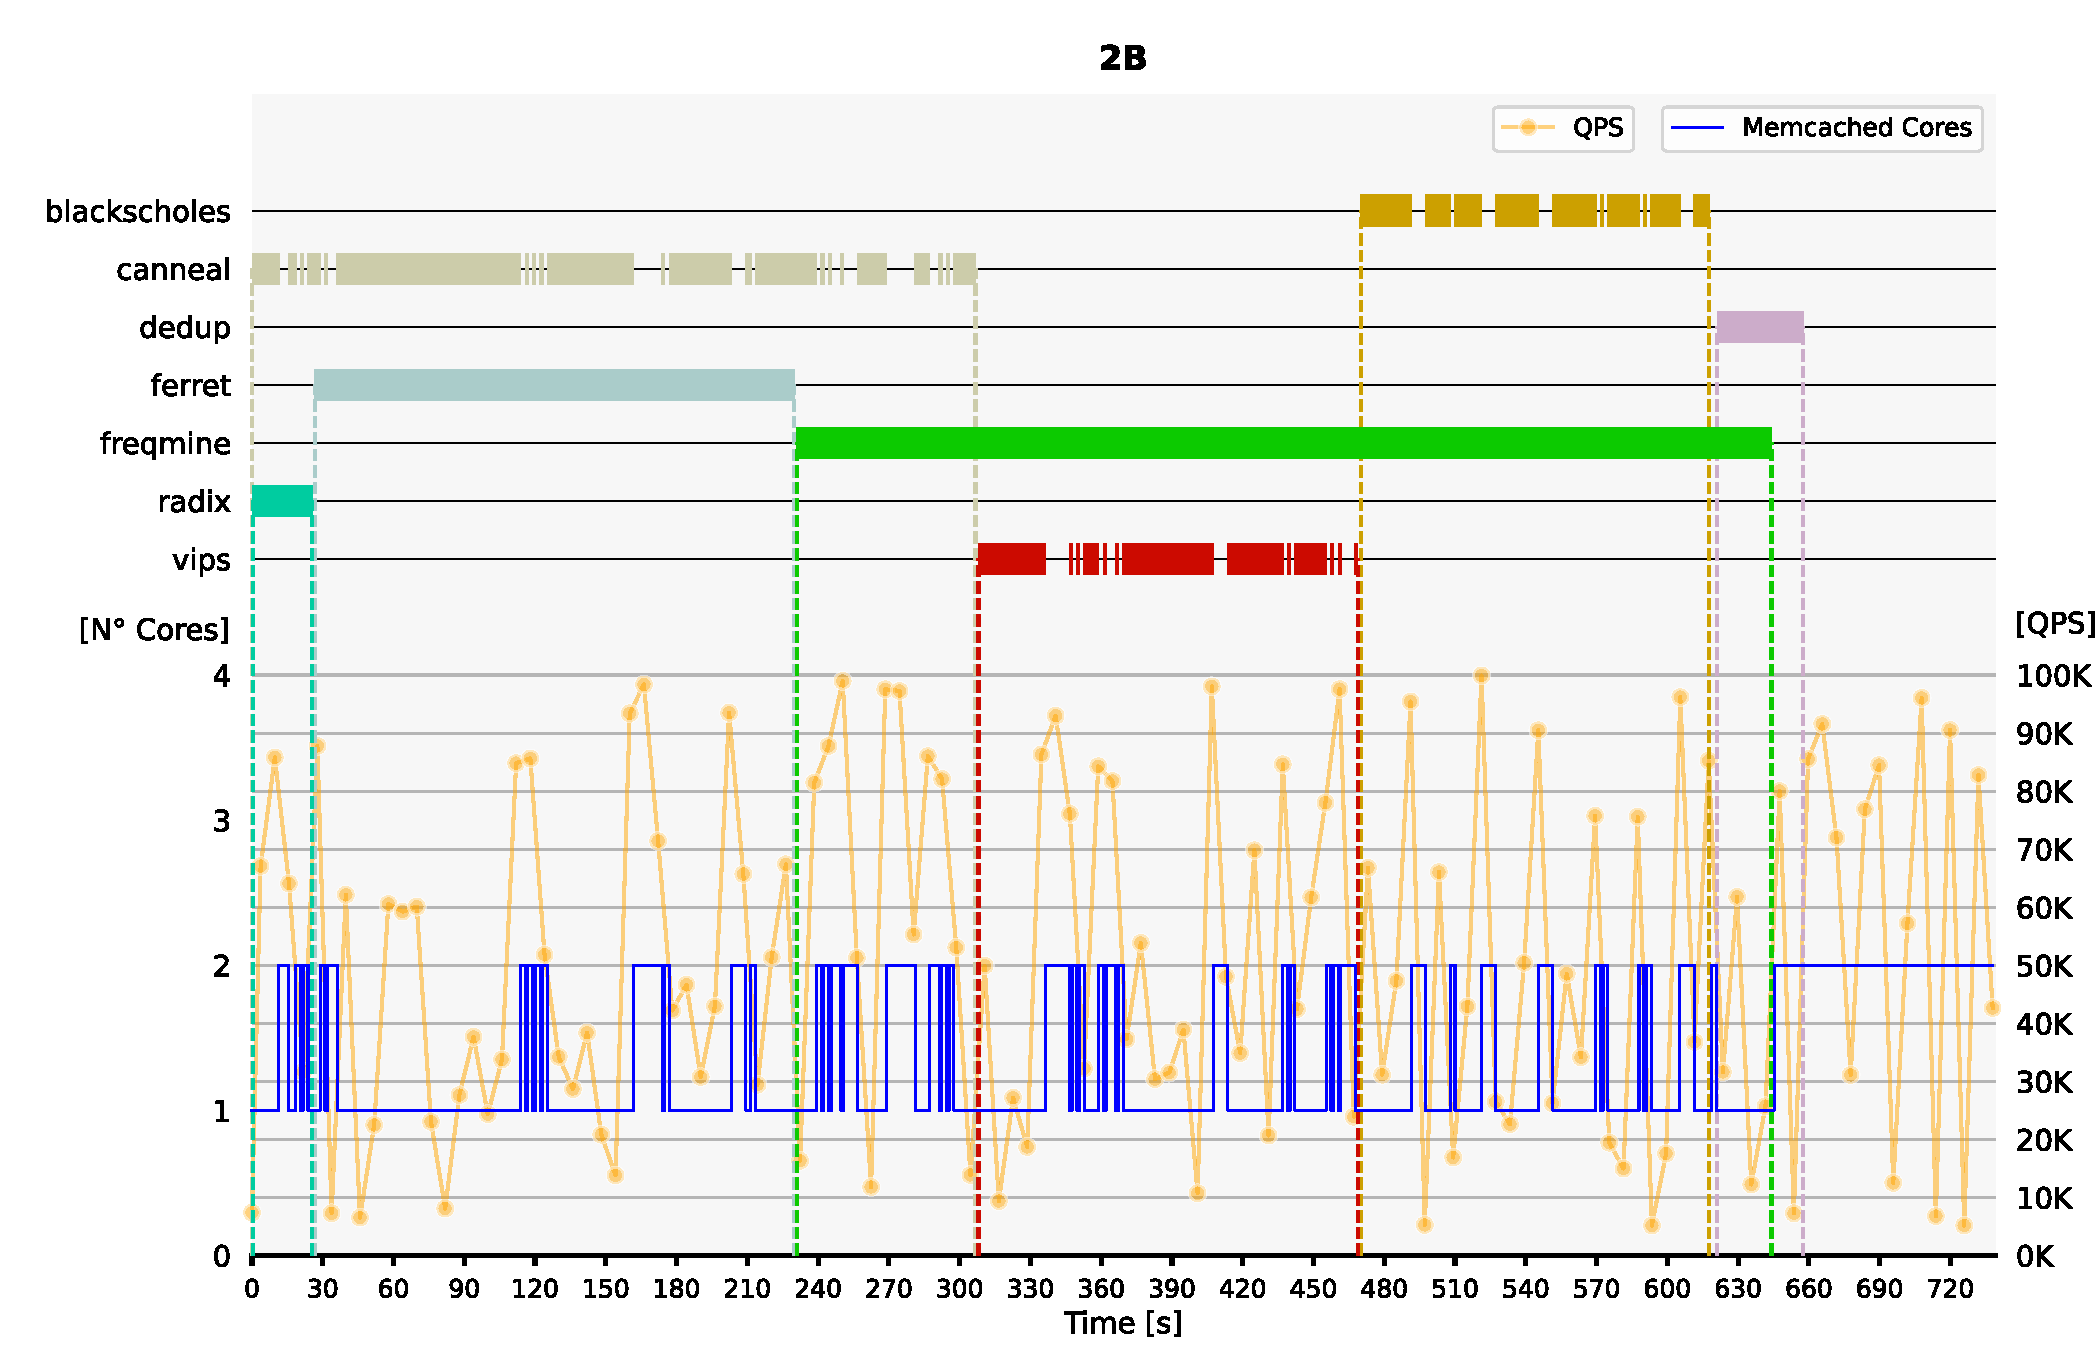
\includegraphics[width=1\linewidth]{figures/part4/plot4_2B.pdf}
        % \caption{Plot 2B}
        \label{fig:plot2B-2}
    \end{figure}

    \begin{figure}[htbp]
        \centering
        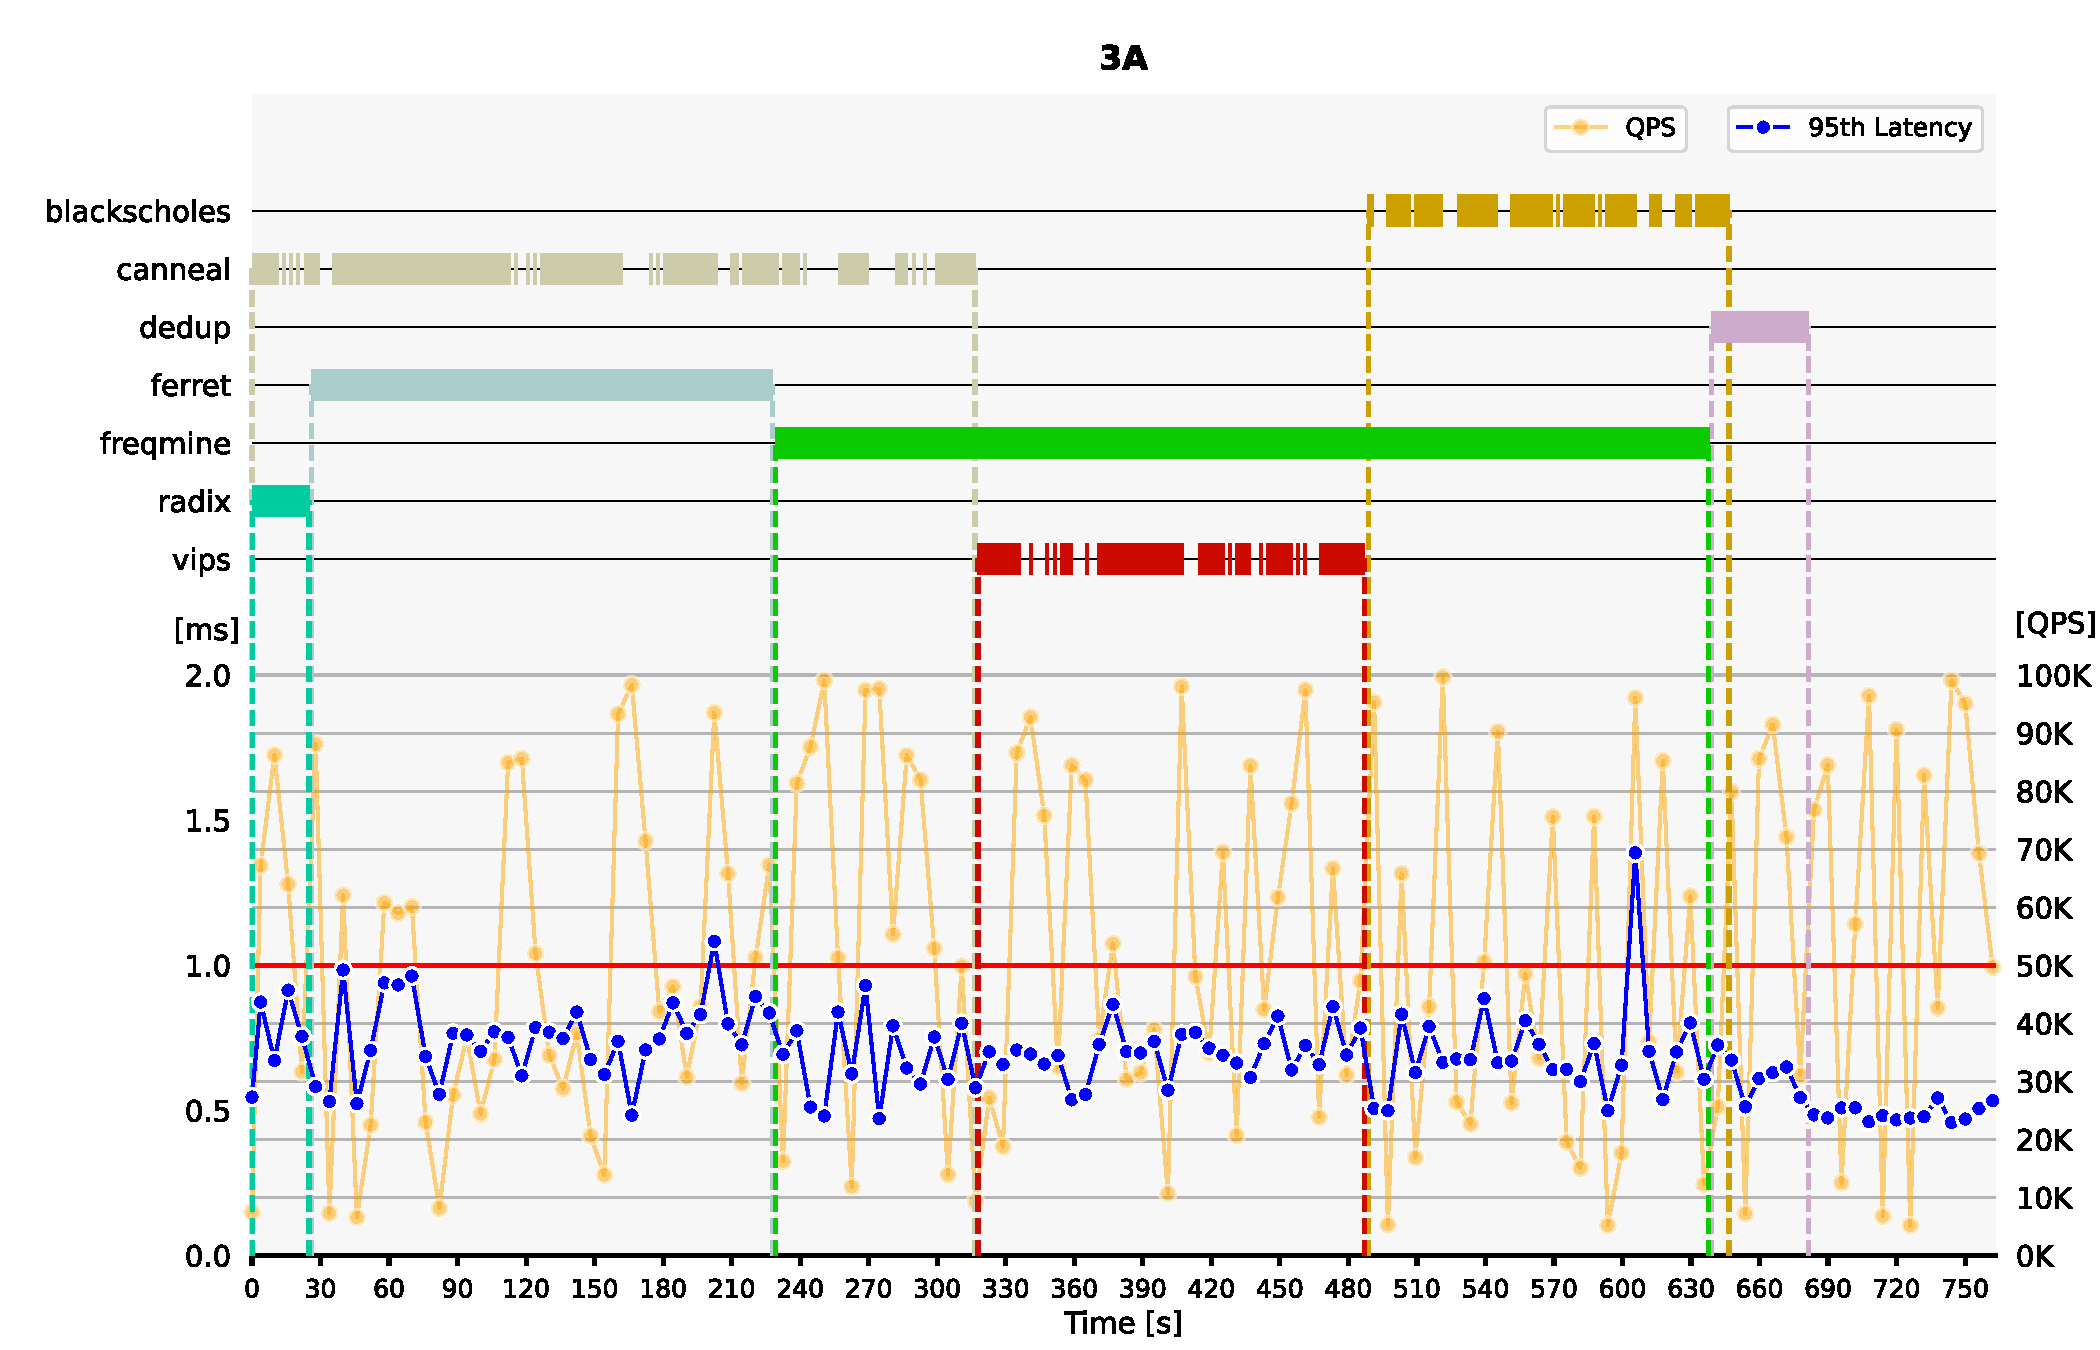
\includegraphics[width=1\linewidth]{figures/part4/plot4_3A.pdf}
        % \caption{Plot 3A}
        \label{fig:plot3A-2}
    \end{figure}

    \begin{figure}[htbp]
        \centering
        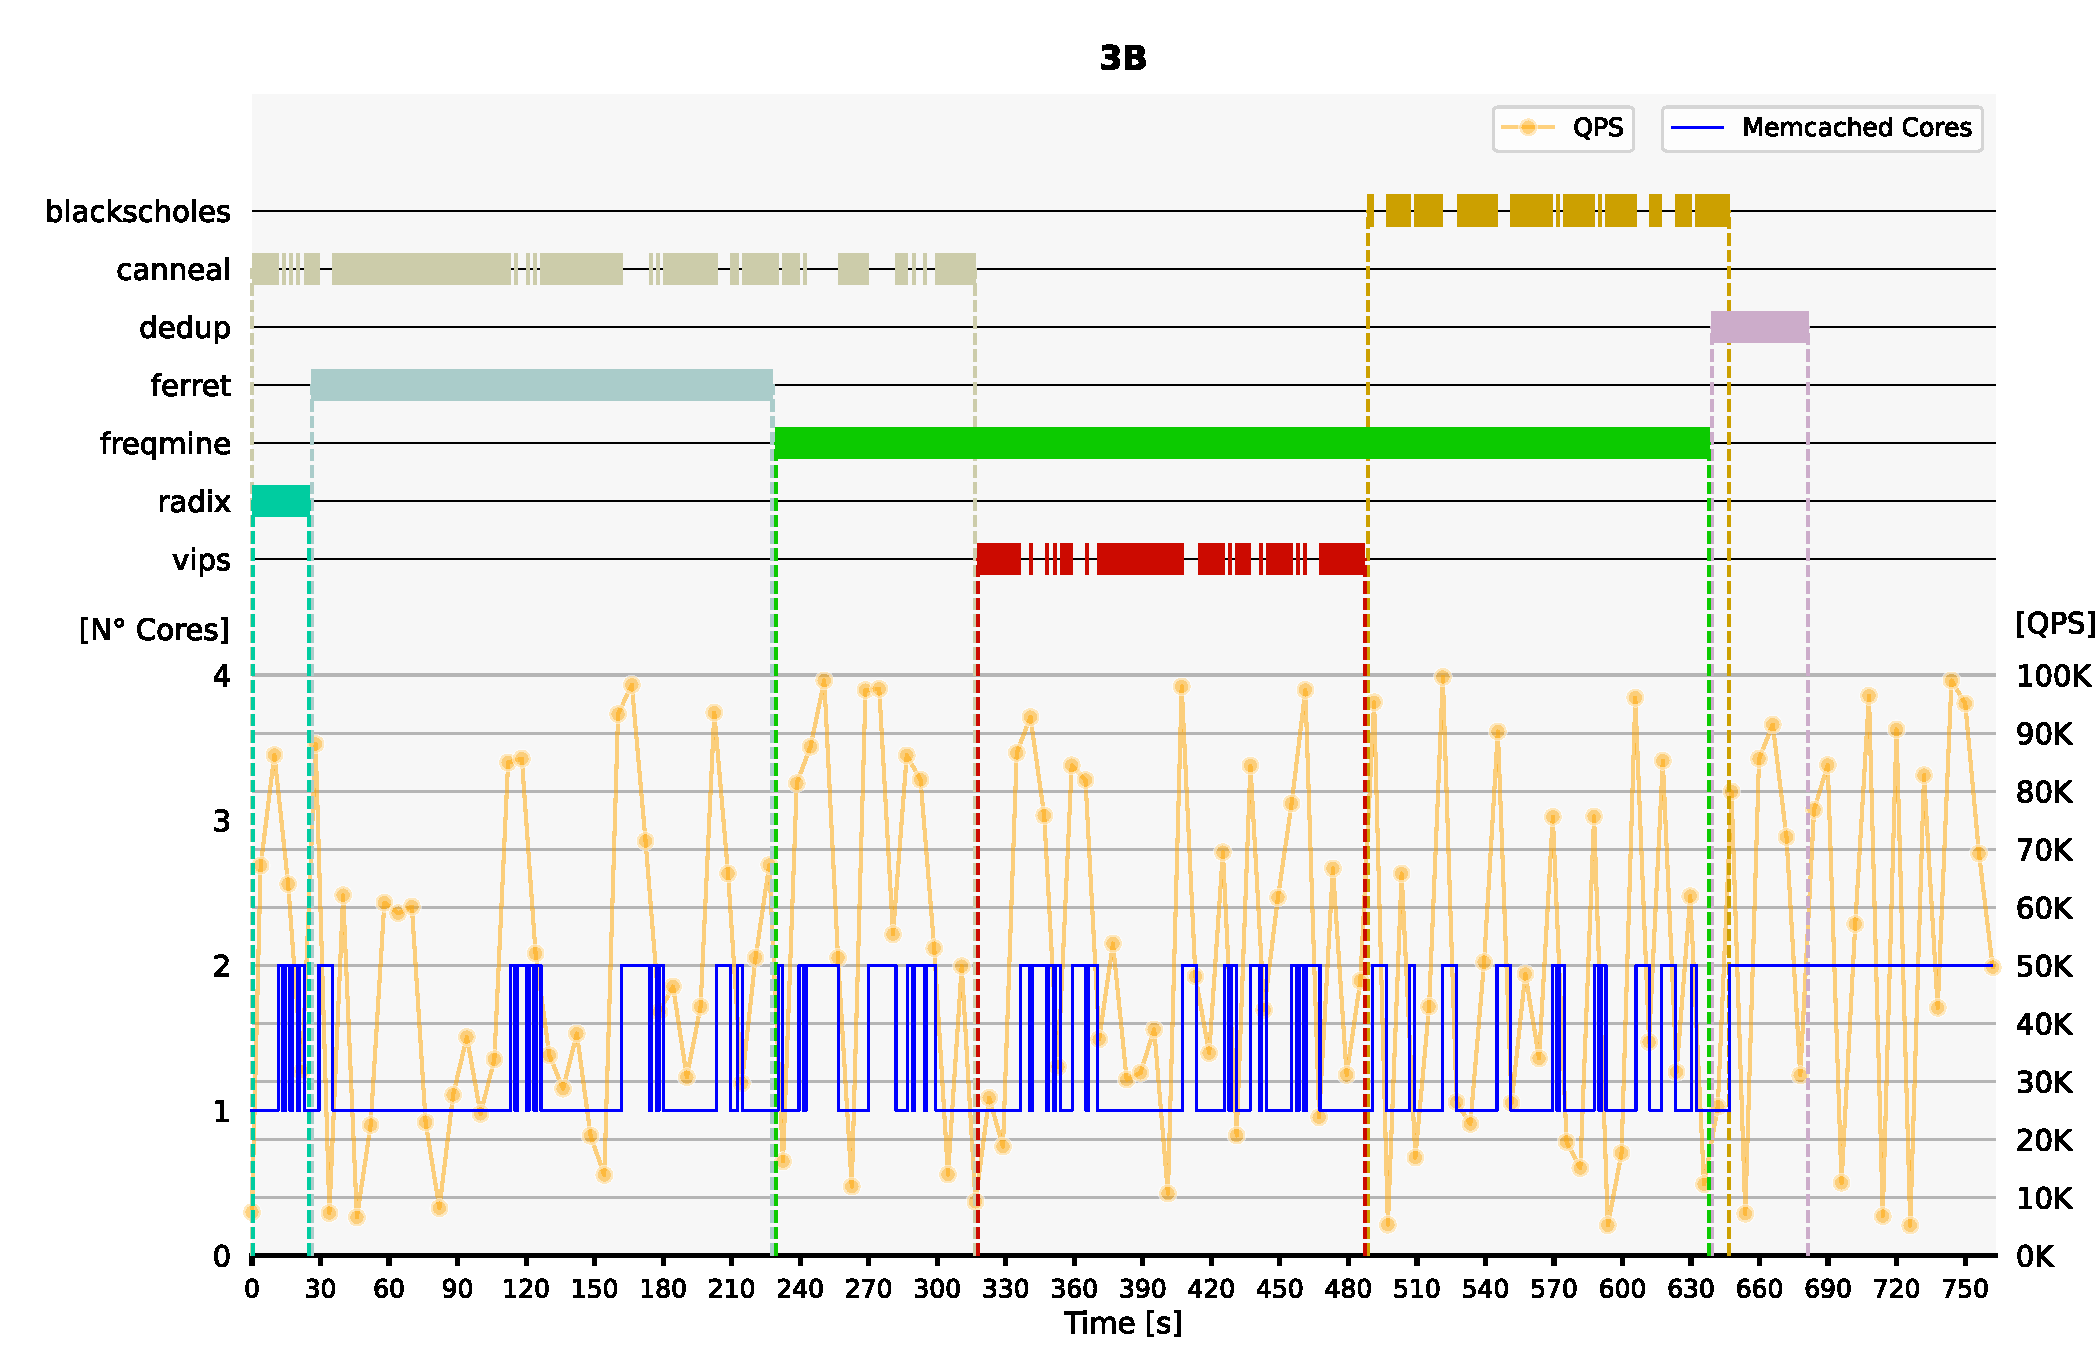
\includegraphics[width=1\linewidth]{figures/part4/plot4_3B.pdf}
        % \caption{Plot 3B}
        \label{fig:plot3B-2}
    \end{figure}
    
\end{enumerate}


\end{document}
